% concatenated from main.tex, 0_config/init_load.tex, 0_config/math_commands.tex, 0_contents/abstract.tex, 0_contents/010introduction.tex, 0_contents/020preliminaries.tex, 0_contents/030methods.tex, 0_contents/060conclusion.tex, 0_contents/0Xappendix/appendix_main.tex
%spider_SIAM-20180701 = arXiv! changed template

\documentclass[11pt]{article}

\usepackage[utf8]{inputenc} % allow utf-8 input

%-----------------------------------
\pdfoutput=1

\usepackage{algorithm}
\usepackage{algorithmic}
% \usepackage[noend]{algpseudocode}
\usepackage{amsmath}
\usepackage{amssymb}
\usepackage{amsthm,amsfonts}
\usepackage{array}
\usepackage{authblk}
\usepackage{babel}
\usepackage{booktabs}
\usepackage{caption}
\usepackage{colortbl}% http://ctan.org/pkg/xcolor
\usepackage{enumitem}
\usepackage[T1]{fontenc}    
\usepackage{framed}
\usepackage{fullpage}
\usepackage{graphicx}
\usepackage[colorlinks, linkcolor=red, anchorcolor=blue, citecolor=blue]{hyperref}
\usepackage{indentfirst}
\usepackage[utf8]{inputenc}
\usepackage{lipsum}        
\usepackage{makecell}
\usepackage{mathrsfs}
\usepackage{mathtools}

\usepackage[framemethod=default]{mdframed}
\usepackage{microtype}     
\usepackage{multicol}
\usepackage{multirow}
\usepackage{natbib}
\usepackage{nicefrac}       % compact symbols for 1/2, etc.
\usepackage{tablefootnote}
\usepackage{url}            % simple URL typesetting
\usepackage{wrapfig,lipsum}
\usepackage{xcolor}         % colors
\usepackage{xspace}



\usepackage{doi}
\usepackage{tikz}
\usetikzlibrary{arrows.meta}
\usetikzlibrary{decorations.pathreplacing}
% \renewcommand{\baselinestretch}{1.1}
\parindent 15pt


% For paper revision:
\newcommand{\xh}[1]{\textcolor[HTML]{66CCFF}{#1}}
\def \dz {\textcolor{red}}
%%%%% NEW MATH DEFINITIONS %%%%%

\usepackage{amsmath,amsfonts,bm}

% Mark sections of captions for referring to divisions of figures

\newcommand{\figleft}{{\em (Left)}}

\newcommand{\name}{{{RDS}}}


\newcommand{\figcenter}{{\em (Center)}}
\newcommand{\figright}{{\em (Right)}}
\newcommand{\figtop}{{\em (Top)}}
\newcommand{\RR}{{\mathbb R}}
\newcommand{\figbottom}{{\em (Bottom)}}
\newcommand{\captiona}{{\em (a)}}
\newcommand{\captionb}{{\em (b)}}
\newcommand{\captionc}{{\em (c)}}
\newcommand{\captiond}{{\em (d)}}

% Highlight a newly defined term
\newcommand{\newterm}[1]{{\bf #1}}

\newcommand{\hanze}[1]{{\textcolor{orange}{#1} }}

\newcommand{\issue}[1]{{\textcolor{purple}{#1} }}
% Figure reference, lower-case.
\def\figref#1{figure~\ref{#1}}
% Figure reference, capital. For start of sentence
\def\Figref#1{Figure~\ref{#1}}
\def\twofigref#1#2{figures \ref{#1} and \ref{#2}}
\def\quadfigref#1#2#3#4{figures \ref{#1}, \ref{#2}, \ref{#3} and \ref{#4}}
% Section reference, lower-case.
\def\secref#1{section~\ref{#1}}
% Section reference, capital.
\def\Secref#1{Section~\ref{#1}}
% Reference to two sections.
\def\twosecrefs#1#2{sections \ref{#1} and \ref{#2}}
% Reference to three sections.
\def\secrefs#1#2#3{sections \ref{#1}, \ref{#2} and \ref{#3}}
% Reference to an equation, lower-case.
%\def\eqref#1{equation~(\ref{#1})}
% Reference to an equation, upper case
%\def\Eqref#1{Equation~(\ref{#1})}
% A raw reference to an equation---avoid using if possible
\def\plaineqref#1{\ref{#1}}
% Reference to a chapter, lower-case.
\def\chapref#1{chapter~\ref{#1}}
% Reference to an equation, upper case.
\def\Chapref#1{Chapter~\ref{#1}}
% Reference to a range of chapters
\def\rangechapref#1#2{chapters\ref{#1}--\ref{#2}}
% Reference to an algorithm, lower-case.
\def\algref#1{algorithm~\ref{#1}}
% Reference to an algorithm, upper case.
\def\Algref#1{Algorithm~\ref{#1}}
\def\twoalgref#1#2{algorithms \ref{#1} and \ref{#2}}
\def\Twoalgref#1#2{Algorithms \ref{#1} and \ref{#2}}
% Reference to a part, lower case
\def\partref#1{part~\ref{#1}}
% Reference to a part, upper case
\def\Partref#1{Part~\ref{#1}}
\def\twopartref#1#2{parts \ref{#1} and \ref{#2}}

\def\ceil#1{\lceil #1 \rceil}
\def\floor#1{\lfloor #1 \rfloor}
\def\1{\bm{1}}
\newcommand{\train}{\mathcal{D}}
\newcommand{\valid}{\mathcal{D_{\mathrm{valid}}}}
\newcommand{\test}{\mathcal{D_{\mathrm{test}}}}

\def\eps{{\epsilon}}

\def\cN{{\mathcal{N}}}
% Random variables
\def\reta{{\textnormal{$\eta$}}}
\def\ra{{\textnormal{a}}}
\def\rb{{\textnormal{b}}}
\def\rc{{\textnormal{c}}}
\def\rd{{\textnormal{d}}}
\def\re{{\textnormal{e}}}
\def\rf{{\textnormal{f}}}
\def\rg{{\textnormal{g}}}
\def\rh{{\textnormal{h}}}
\def\ri{{\textnormal{i}}}
\def\rj{{\textnormal{j}}}
\def\rk{{\textnormal{k}}}
\def\rl{{\textnormal{l}}}
% rm is already a command, just don't name any random variables m
\def\rn{{\textnormal{n}}}
\def\ro{{\textnormal{o}}}
\def\rp{{\textnormal{p}}}
\def\rq{{\textnormal{q}}}
\def\rr{{\textnormal{r}}}
\def\rs{{\textnormal{s}}}
\def\rt{{\textnormal{t}}}
\def\ru{{\textnormal{u}}}
\def\rv{{\textnormal{v}}}
\def\rw{{\textnormal{w}}}
\def\rx{{\textnormal{x}}}
\def\ry{{\textnormal{y}}}
\def\rz{{\textnormal{z}}}

% Random vectors
\def\rvepsilon{{\mathbf{\epsilon}}}
\def\rvtheta{{\mathbf{\theta}}}
\def\rvzeta{{\mathbf{\zeta}}}
\def\rva{{\mathbf{a}}}
\def\rvb{{\mathbf{b}}}
\def\rvc{{\mathbf{c}}}
\def\rvd{{\mathbf{d}}}
\def\rve{{\mathbf{e}}}
\def\rvf{{\mathbf{f}}}
\def\rvg{{\mathbf{g}}}
\def\rvh{{\mathbf{h}}}
\def\rvu{{\mathbf{i}}}
\def\rvj{{\mathbf{j}}}
\def\rvk{{\mathbf{k}}}
\def\rvl{{\mathbf{l}}}
\def\rvm{{\mathbf{m}}}
\def\rvn{{\mathbf{n}}}
\def\rvo{{\mathbf{o}}}
\def\rvp{{\mathbf{p}}}
\def\rvq{{\mathbf{q}}}
\def\rvr{{\mathbf{r}}}
\def\rvs{{\mathbf{s}}}
\def\rvt{{\mathbf{t}}}
\def\rvu{{\mathbf{u}}}
\def\rvv{{\mathbf{v}}}
\def\rvw{{\mathbf{w}}}
\def\rvx{{\mathbf{x}}}
\def\rvy{{\mathbf{y}}}
\def\rvz{{\mathbf{z}}}

% Elements of random vectors
\def\erva{{\textnormal{a}}}
\def\ervb{{\textnormal{b}}}
\def\ervc{{\textnormal{c}}}
\def\ervd{{\textnormal{d}}}
\def\erve{{\textnormal{e}}}
\def\ervf{{\textnormal{f}}}
\def\ervg{{\textnormal{g}}}
\def\ervh{{\textnormal{h}}}
\def\ervi{{\textnormal{i}}}
\def\ervj{{\textnormal{j}}}
\def\ervk{{\textnormal{k}}}
\def\ervl{{\textnormal{l}}}
\def\ervm{{\textnormal{m}}}
\def\ervn{{\textnormal{n}}}
\def\ervo{{\textnormal{o}}}
\def\ervp{{\textnormal{p}}}
\def\ervq{{\textnormal{q}}}
\def\ervr{{\textnormal{r}}}
\def\ervs{{\textnormal{s}}}
\def\ervt{{\textnormal{t}}}
\def\ervu{{\textnormal{u}}}
\def\ervv{{\textnormal{v}}}
\def\ervw{{\textnormal{w}}}
\def\ervx{{\textnormal{x}}}
\def\ervy{{\textnormal{y}}}
\def\ervz{{\textnormal{z}}}

% Random matrices
\def\rmA{{\mathbf{A}}}
\def\rmB{{\mathbf{B}}}
\def\rmC{{\mathbf{C}}}
\def\rmD{{\mathbf{D}}}
\def\rmE{{\mathbf{E}}}
\def\rmF{{\mathbf{F}}}
\def\rmG{{\mathbf{G}}}
\def\rmH{{\mathbf{H}}}
\def\rmI{{\mathbf{I}}}
\def\rmJ{{\mathbf{J}}}
\def\rmK{{\mathbf{K}}}
\def\rmL{{\mathbf{L}}}
\def\rmM{{\mathbf{M}}}
\def\rmN{{\mathbf{N}}}
\def\rmO{{\mathbf{O}}}
\def\rmP{{\mathbf{P}}}
\def\rmQ{{\mathbf{Q}}}
\def\rmR{{\mathbf{R}}}
\def\rmS{{\mathbf{S}}}
\def\rmT{{\mathbf{T}}}
\def\rmU{{\mathbf{U}}}
\def\rmV{{\mathbf{V}}}
\def\rmW{{\mathbf{W}}}
\def\rmX{{\mathbf{X}}}
\def\rmY{{\mathbf{Y}}}
\def\rmZ{{\mathbf{Z}}}

% Elements of random matrices
\def\ermA{{\textnormal{A}}}
\def\ermB{{\textnormal{B}}}
\def\ermC{{\textnormal{C}}}
\def\ermD{{\textnormal{D}}}
\def\ermE{{\textnormal{E}}}
\def\ermF{{\textnormal{F}}}
\def\ermG{{\textnormal{G}}}
\def\ermH{{\textnormal{H}}}
\def\ermI{{\textnormal{I}}}
\def\ermJ{{\textnormal{J}}}
\def\ermK{{\textnormal{K}}}
\def\ermL{{\textnormal{L}}}
\def\ermM{{\textnormal{M}}}
\def\ermN{{\textnormal{N}}}
\def\ermO{{\textnormal{O}}}
\def\ermP{{\textnormal{P}}}
\def\ermQ{{\textnormal{Q}}}
\def\ermR{{\textnormal{R}}}
\def\ermS{{\textnormal{S}}}
\def\cR{{\mathcal{R}}}
\def\EE{{\mathbb{E}}}
\def\ermT{{\textnormal{T}}}
\def\ermU{{\textnormal{U}}}
\def\ermV{{\textnormal{V}}}
\def\ermW{{\textnormal{W}}}
\def\ermX{{\textnormal{X}}}
\def\ermY{{\textnormal{Y}}}
\def\ermZ{{\textnormal{Z}}}

% Vectors
\def\vzero{{\bm{0}}}
\def\vone{{\bm{1}}}
\def\vmu{{\bm{\mu}}}
\def\vtheta{{\bm{\theta}}}
\def\vrho{{\bm{\rho}}}
\def\vzeta{{\bm{\zeta}}}
\def\va{{\bm{a}}}
\def\vb{{\bm{b}}}
\def\vc{{\bm{c}}}
\def\vd{{\bm{d}}}
\def\ve{{\bm{e}}}
\def\vf{{\bm{f}}}
\def\vg{{\bm{g}}}
\def\vh{{\bm{h}}}
\def\vi{{\bm{i}}}
\def\vj{{\bm{j}}}
\def\vk{{\bm{k}}}
\def\vl{{\bm{l}}}
\def\vm{{\bm{m}}}
\def\vn{{\bm{n}}}
\def\vo{{\bm{o}}}
\def\vp{{\bm{p}}}
\def\vq{{\bm{q}}}
\def\vr{{\bm{r}}}
\def\vs{{\bm{s}}}
\def\vt{{\bm{t}}}
\def\vu{{\bm{u}}}
\def\vv{{\bm{v}}}
\def\vw{{\bm{w}}}
\def\vx{{\bm{x}}}
\def\vy{{\bm{y}}}
\def\vz{{\bm{z}}}
\def\vmu{{\bm{\mu}}}
\def\vsigma{{\bm{\sigma}}}

% Elements of vectors
\def\evalpha{{\alpha}}
\def\evbeta{{\beta}}
\def\evepsilon{{\epsilon}}
\def\evlambda{{\lambda}}
\def\evomega{{\omega}}
\def\evmu{{\mu}}
\def\evpsi{{\psi}}
\def\evsigma{{\sigma}}
\def\evtheta{{\theta}}
\def\eva{{a}}
\def\evb{{b}}
\def\evc{{c}}
\def\evd{{d}}
\def\eve{{e}}
\def\evf{{f}}
\def\evg{{g}}
\def\evh{{h}}
\def\evi{{i}}
\def\evj{{j}}
\def\evk{{k}}
\def\evl{{l}}
\def\evm{{m}}
\def\evn{{n}}
\def\evo{{o}}
\def\evp{{p}}
\def\evq{{q}}
\def\evr{{r}}
\def\evs{{s}}
\def\evt{{t}}
\def\evu{{u}}
\def\evv{{v}}
\def\evw{{w}}
\def\evx{{x}}
\def\evy{{y}}
\def\evz{{z}}

% Matrix
\def\mA{{\bm{A}}}
\def\mB{{\bm{B}}}
\def\mC{{\bm{C}}}
\def\mD{{\bm{D}}}
\def\mE{{\bm{E}}}
\def\mF{{\bm{F}}}
\def\mG{{\bm{G}}}
\def\mH{{\bm{H}}}
\def\mI{{\bm{I}}}
\def\mJ{{\bm{J}}}
\def\mK{{\bm{K}}}
\def\mL{{\bm{L}}}
\def\mM{{\bm{M}}}
\def\mN{{\bm{N}}}
\def\mO{{\bm{O}}}
\def\mP{{\bm{P}}}
\def\mQ{{\bm{Q}}}
\def\mR{{\bm{R}}}
\def\mS{{\bm{S}}}
\def\mT{{\bm{T}}}
\def\mU{{\bm{U}}}
\def\mV{{\bm{V}}}
\def\mW{{\bm{W}}}
\def\mX{{\bm{X}}}
\def\mY{{\bm{Y}}}
\def\mZ{{\bm{Z}}}
\def\mBeta{{\bm{\beta}}}
\def\mPhi{{\bm{\Phi}}}
\def\mLambda{{\bm{\Lambda}}}
\def\mSigma{{\bm{\Sigma}}}

% Tensor
\DeclareMathAlphabet{\mathsfit}{\encodingdefault}{\sfdefault}{m}{sl}
\SetMathAlphabet{\mathsfit}{bold}{\encodingdefault}{\sfdefault}{bx}{n}
\newcommand{\tens}[1]{\bm{\mathsfit{#1}}}
\def\tA{{\tens{A}}}
\def\tB{{\tens{B}}}
\def\tC{{\tens{C}}}
\def\tD{{\tens{D}}}
\def\tE{{\tens{E}}}
\def\tF{{\tens{F}}}
\def\tG{{\tens{G}}}
\def\tH{{\tens{H}}}
\def\tI{{\tens{I}}}
\def\tJ{{\tens{J}}}
\def\tK{{\tens{K}}}
\def\tL{{\tens{L}}}
\def\tM{{\tens{M}}}
\def\tN{{\tens{N}}}
\def\tO{{\tens{O}}}
\def\tP{{\tens{P}}}
\def\tQ{{\tens{Q}}}
\def\tR{{\tens{R}}}
\def\tS{{\tens{S}}}
\def\tT{{\tens{T}}}
\def\tU{{\tens{U}}}
\def\tV{{\tens{V}}}
\def\tW{{\tens{W}}}
\def\tX{{\tens{X}}}
\def\tY{{\tens{Y}}}
\def\tZ{{\tens{Z}}}


% Graph
\def\gA{{\mathcal{A}}}
\def\gB{{\mathcal{B}}}
\def\gC{{\mathcal{C}}}
\def\gD{{\mathcal{D}}}
\def\gE{{\mathcal{E}}}
\def\gF{{\mathcal{F}}}
\def\gG{{\mathcal{G}}}
\def\gH{{\mathcal{H}}}
\def\gI{{\mathcal{I}}}
\def\gJ{{\mathcal{J}}}
\def\gK{{\mathcal{K}}}
\def\gL{{\mathcal{L}}}
\def\gM{{\mathcal{M}}}
\def\gN{{\mathcal{N}}}
\def\gO{{\mathcal{O}}}
\def\gP{{\mathcal{P}}}
\def\gQ{{\mathcal{Q}}}
\def\gR{{\mathcal{R}}}
\def\gS{{\mathcal{S}}}
\def\gT{{\mathcal{T}}}
\def\gU{{\mathcal{U}}}
\def\gV{{\mathcal{V}}}
\def\gW{{\mathcal{W}}}
\def\gX{{\mathcal{X}}}
\def\gY{{\mathcal{Y}}}
\def\gZ{{\mathcal{Z}}}

% Sets
\def\sA{{\mathbb{A}}}
\def\sB{{\mathbb{B}}}
\def\sC{{\mathbb{C}}}
\def\sD{{\mathbb{D}}}
% Don't use a set called E, because this would be the same as our symbol
% for expectation.
\def\sF{{\mathbb{F}}}
\def\sG{{\mathbb{G}}}
\def\sH{{\mathbb{H}}}
\def\sI{{\mathbb{I}}}
\def\sJ{{\mathbb{J}}}
\def\sK{{\mathbb{K}}}
\def\sL{{\mathbb{L}}}
\def\sM{{\mathbb{M}}}
\def\sN{{\mathbb{N}}}
\def\sO{{\mathbb{O}}}
\def\sP{{\mathbb{P}}}
\def\sQ{{\mathbb{Q}}}
\def\sR{{\mathbb{R}}}
\def\sS{{\mathbb{S}}}
\def\sT{{\mathbb{T}}}
\def\sU{{\mathbb{U}}}
\def\sV{{\mathbb{V}}}
\def\sW{{\mathbb{W}}}
\def\sX{{\mathbb{X}}}
\def\sY{{\mathbb{Y}}}
\def\sZ{{\mathbb{Z}}}

% Entries of a matrix
\def\emLambda{{\Lambda}}
\def\emA{{A}}
\def\emB{{B}}
\def\emC{{C}}
\def\emD{{D}}
\def\emE{{E}}
\def\emF{{F}}
\def\emG{{G}}
\def\emH{{H}}
\def\emI{{I}}
\def\emJ{{J}}
\def\emK{{K}}
\def\emL{{L}}
\def\emM{{M}}
\def\emN{{N}}
\def\emO{{O}}
\def\emP{{P}}
\def\emQ{{Q}}
\def\emR{{R}}
\def\emS{{S}}
\def\emT{{T}}
\def\emU{{U}}
\def\emV{{V}}
\def\emW{{W}}
\def\emX{{X}}
\def\emY{{Y}}
\def\emZ{{Z}}
\def\emSigma{{\Sigma}}

% entries of a tensor
% Same font as tensor, without \bm wrapper
\newcommand{\etens}[1]{\mathsfit{#1}}
\def\etLambda{{\etens{\Lambda}}}
\def\etA{{\etens{A}}}
\def\etB{{\etens{B}}}
\def\etC{{\etens{C}}}
\def\etD{{\etens{D}}}
\def\etE{{\etens{E}}}
\def\etF{{\etens{F}}}
\def\etG{{\etens{G}}}
\def\etH{{\etens{H}}}
\def\etI{{\etens{I}}}
\def\etJ{{\etens{J}}}
\def\etK{{\etens{K}}}
\def\etL{{\etens{L}}}
\def\etM{{\etens{M}}}
\def\etN{{\etens{N}}}
\def\etO{{\etens{O}}}
\def\etP{{\etens{P}}}
\def\etQ{{\etens{Q}}}
\def\etR{{\etens{R}}}
\def\etS{{\etens{S}}}
\def\etT{{\etens{T}}}
\def\etU{{\etens{U}}}
\def\etV{{\etens{V}}}
\def\etW{{\etens{W}}}
\def\etX{{\etens{X}}}
\def\etY{{\etens{Y}}}
\def\etZ{{\etens{Z}}}

%

\newcommand{\grad}{\ensuremath{\nabla}}
\newcommand*\circled[1]{\tikz[baseline=(char.base)]{
            \node[shape=circle,draw,inner sep=1pt] (char) {\tiny{#1}};}}
% The true underlying data generating distribution
\newcommand{\pdata}{p_{\rm{data}}}
% The empirical distribution defined by the training set
\newcommand{\ptrain}{\hat{p}_{\rm{data}}}
\newcommand{\Ptrain}{\hat{P}_{\rm{data}}}
% The model distribution
\newcommand{\pmodel}{p_{\rm{model}}}
\newcommand{\Pmodel}{P_{\rm{model}}}
\newcommand{\ptildemodel}{\tilde{p}_{\rm{model}}}
% Stochastic autoencoder distributions
\newcommand{\pencode}{p_{\rm{encoder}}}
\newcommand{\pdecode}{p_{\rm{decoder}}}
\newcommand{\precons}{p_{\rm{reconstruct}}}

\newcommand{\laplace}{\mathrm{Laplace}} % Laplace distribution

\newcommand{\E}{\mathbb{E}}
\newcommand{\Ls}{\mathcal{L}}
\newcommand{\R}{\mathbb{R}}
\newcommand{\emp}{\tilde{p}}
\newcommand{\lr}{\alpha}
\newcommand{\reg}{\lambda}
\newcommand{\rect}{\mathrm{rectifier}}
\newcommand{\softmax}{\mathrm{softmax}}
\newcommand{\sigmoid}{\sigma}
\newcommand{\softplus}{\zeta}
\newcommand{\KL}[2]{\mathrm{KL}\left(#1 \big\| #2\right)}
\newcommand{\FI}[2]{\mathrm{FI}\left(#1 \| #2\right)}
\newcommand{\TVD}[2]{\mathrm{TV}\left(#1, #2\right)}
\newcommand{\Var}{\mathrm{Var}}
\newcommand{\standarderror}{\mathrm{SE}}
\newcommand{\Cov}{\mathrm{Cov}}
% Wolfram Mathworld says $L^2$ is for function spaces and $\ell^2$ is for vectors
% But then they seem to use $L^2$ for vectors throughout the site, and so does
% wikipedia.
\newcommand{\normlzero}{L^0}
\newcommand{\normlone}{L^1}
\newcommand{\normltwo}{L^2}
\newcommand{\normlp}{L^p}
\newcommand{\normmax}{L^\infty}

\newcommand{\parents}{Pa} % See usage in notation.tex. Chosen to match Daphne's book.


\newcommand{\der}{\mathrm{d}}
\newcommand{\fder}{\mathrm{D}}
\newcommand{\rgrad}{\mathrm{grad}}


\DeclareMathOperator*{\argmax}{arg\,max}
\DeclareMathOperator*{\argmin}{arg\,min}

\DeclareMathOperator{\sign}{sign}
\DeclareMathOperator{\Tr}{Tr}
\let\ab\allowbreak

% Table settings

\makeatletter
\def\thickhline{%
  \noalign{\ifnum0=`}\fi\hrule \@height \thickarrayrulewidth \futurelet
   \reserved@a\@xthickhline}
\def\@xthickhline{\ifx\reserved@a\thickhline
               \vskip\doublerulesep
               \vskip-\thickarrayrulewidth
             \fi
      \ifnum0=`{\fi}}
\makeatother

\newlength{\thickarrayrulewidth}
\setlength{\thickarrayrulewidth}{3\arrayrulewidth}

\newcommand{\tabitem}{~~\llap{\textbullet}~~}


% Lemma settings


\newtheorem{lemma}{Lemma}[section]
\newtheorem{theorem}[lemma]{Theorem}
\newtheorem{corollary}[lemma]{Corollary}
\newtheorem{proposition}[lemma]{Proposition}
\newtheorem{fact}[lemma]{Fact}
\newtheorem{remark}{Remark}
\newtheorem{assumption}{Assumption}
\newtheorem{definition}{Definition}

%Specific Notations for Sampling along the Reverse Process with Recursive Score Estimation
% \algnewcommand{\IfThenElse}[3]{% \IfThenElse{<if>}{<then>}{<else>}
% \State \algorithmicif\ #1\ \algorithmicthen\ #2\ \algorithmicelse\ #3}

\newcommand{\rbkwx}{\rvx^{\gets}}
\newcommand{\bkwx}{\vx^{\gets}}
\newcommand{\rbkwv}{\rvv^{\gets}}
\newcommand{\bkwp}{p^{\gets}}
\newcommand{\ourmethod}{\text{RS-DMC}}



%%%%%%Revised


\newcommand*\samethanks[1][\value{footnote}]{\footnotemark[#1]}


% \title{\LARGE Recursive Score Estimation Accelerates Diffusion-Based \\ Monte Carlo}

% \title{Faster Sampling without Isoperimetry \\ via Diffusion-based Monte Carlo}

\title{Multi-step Consistency Models: Fast Generation with  \\ Theoretical Guarantees}

% \title{Scaling Reverse Diffusion Monte Carlo \\ with Recursive Score Estimation}

\author[$\dagger$]{\normalsize Nishant Jain\thanks{Equal Contribution, Mail to \href{nj27@illinois.edu}{nj27@illinois.edu}, \href{xhuangck@connect.ust.hk}{xuh031@ucsd.edu} }}
\author[$\S$]{Xunpeng Huang\samethanks}
% \author[$\dagger$]{Hanze Dong}
\author[$\S$]{Yian Ma}
\author[$\dagger$]{Tong Zhang}

\affil[$\dagger$]{University of Illinois Urbana-Champaign}
% \affil[$\S$]{The University of Hong Kong}
\affil[$\S$]{University of California San Diego}
% \affil[$\ddag$]{University of Illinois Urbana-Champaign}
%\affil[ ]{\texttt {\{xhuangck,hendry.dong\}@connect.ust.hk, dzou@cs.hku.hk}}
%\affil[ ]{\texttt{yianma@ucsd.edu, tongzhang@ust.hk}}

\begin{document}

\date{}
\maketitle


\begin{abstract}
 Consistency models have recently emerged as a compelling alternative to traditional SDE-based diffusion models. They offer a significant acceleration in generation by producing high-quality samples in very few steps. Despite their empirical success, a proper theoretic justification for their speed-up is still lacking. 
 % In this work, we provide the analysis that bridges this gap, showing that given a consistency model which can map the input at a given time to arbitrary timestamps along the reverse trajectory, one can achieve a KL divergence of order \( O(\varepsilon) \) using only \( O\left(\log\left(\frac{d}{\varepsilon}\right)\right) \) iterations with constant step size.
 In this work, we address the gap by providing a theoretical analysis of consistency models capable of mapping inputs at a given time to arbitrary points along the reverse trajectory. We show that one can achieve a KL divergence of order \( O(\varepsilon^2) \) using only \( O\left(\log\left(d/\varepsilon\right)\right) \) iterations with a constant step size. 
 % This result highlights the potential for efficient inference in consistency-based generative models with provable accuracy guarantees.
 Additionally, under minimal assumptions on the data distribution (non-smooth case)—an increasingly common setting in recent diffusion model analyses—we show that a similar KL convergence guarantee can be obtained, with the number of steps scaling as \( O\left(d \log\left(d/\varepsilon\right)\right) \). 
 Going further, we also provide a theoretical analysis for estimation of such consistency models, concluding that accurate learning is feasible using small discretization steps, both in smooth and non-smooth settings. Notably, our results for the non-smooth case yield best-in-class convergence rates compared to existing SDE/ODE-based analyses under minimal assumptions.

\end{abstract}


\section{Introduction}
% \xh{provide backgrounds}
Lately, diffusion models \cite{sohl2015deep} have become an important topic of research in computer vision and generative modelling \cite{song2019generative, croitoru2023diffusion, lugmayr2022repaint, song2020denoising, nichol2021glide, song2021maximum, ho2020denoising}, with applications ranging from generating images or videos \cite{epstein2023diffusion, chen2023control} controllably to other areas like drug/protein design \cite{gruver2023protein, guo2024diffusion}. These models comprise a forward process that gradually adds noise to the data, and then the generation is done by the corresponding denoising process, which is sometimes referred to as the reverse/generation process.
These forward/reverse processes can either be seen as transition kernels \cite{huang2024reverse, song2020denoising, ho2020denoising}\ or instead modeled as stochastic differential equations (SDEs) \cite{song2020score, song2020sliced, song2021maximum, chen2022sampling}. 
This is popularly referred as \textit{score based generative modeling} due to its reliance on the neural-network parameterized \textit{score function}, which at a given time instant is the gradient of log probability of the marginal distribution corresponding that time.

% \xh{lead to ODE-based -> consistency from high-level} 
Following from the particle-density transition property,~\cite{song2020score} firstly argued that score-based diffusion method can be implemented by an ordinary differential equation (ODE) version.
That means, under the unbiased score estimation, the ODE-based generation will share the same marginal distribution of the particles as those in the SDE-based generations.
From a practical perspective, ODE-based methods can often bring the underlying distribution of particles closer to the data distribution faster than SDE-based methods while maintaining comparable generation quality~\cite{lu2022dpm, zhou2024fast, zhang2022fast}.
Moreover, researchers appreciate the deterministic update property in ODE-based methods since all the randomness is left in the particle initialization, which inspires the proposal of consistency models~\cite{song2023consistency}.

% \xh{introduce consistency alg idea, and show the inference complexity remains loose, propose the theoretical problem}
Motivated by distilling the deterministic mapping from ODE-based diffusion models,
the original consistency model paper \cite{song2023consistency} takes any point along the probability flow ODE to the start \textit{i.e.} the true data distribution with single-step generation function.
Following the attention growth, a recent work \cite{kim2023consistency} attempted to improve the consistency model by extending the consistency function to any timestamp pair along the reverse ODE trajectory and consequently proposed a multi-step training scheme to achieve this, showing empirical effectiveness. 
From a theoretical perspective, \cite{dou2024theory, li2024towards} investigates the sample efficiency or the number of iterations to train such consistency models.
% [summarize what \cite{dou2024theory, li2024towards} investigate in one sentence,e.g., xxx investigate sample efficiency/training step for consistency ...]. 
However, the essential advantage of the consistency model in the inference process remains unknown. 
Although~\cite{lyu2024sampling} provides some initial exploration for the inference efficiency of the consistency model, for achieving the convergence, an $\tilde{O}(\varepsilon^2)$ step size is required that shares the same order as that in typical SDE or ODE-based inference algorithm.
That result can neither show the advantages of introducing the deterministic update distillation nor match the real practice experience. 
Therefore, a natural question is raised:
\begin{quote}
    \emph{Can the consistency model achieve convergence with a larger step size, matching the real practice experience, and what kind of convergence will it achieve?}
\end{quote}


% \xh{To show how we can solve this problem intuitively.}
In this work, we argue that the inference of consistency models via an adapted version of the multi-step updates allows a constant-level step size, which leads to a linear KL convergence toward the original data distribution under minimal smooth assumptions.
Specifically, {with this setup, we show that at the inference time, one can achieve $O(\varepsilon^2)$ error with a constant step size. We provide this analysis for two scenarios: a) having popular assumptions used in the diffusion model analysis \cite{chen2022sampling,song2020score,xu2024provably,lyu2024sampling}, which includes Lipschitzness of the score function, small score estimation error, finite second moment, and b) without assuming that the score function is Lipschitz \cite{chen2023improved, benton2024nearly}  a scenario that is recently considered and deemed closer to the to real-world applications.} We are able to achieve this convergence by using the multi-step generation where after every application of the consistency model, there is a noising step during inference. Intuitively, this noise is effective in cancelling the accumulative score approximation error. Along, with this, another major ingredient is the modified formulation of the original consistency model that can map a sample from a given time instant to any arbitrary instant along the reverse ODE. We thereby analyse a modified multi-step sampling (version adapted to this formulation) in the KL divergence. 
% \xh{Then, provide why we achieve the linearly convergence, e.g.,   mention, we use a noising step in the inference to cancel the accumulative score approximation error and we consider a modified formulation of the original consistency model that can map a sample from a given time instant to any arbitrary instant along the reverse ODE and analyse an adapted version of the multi-step sampling in the KL divergence. }






\noindent
 We summarize the major contributions of this work as follows:


\begin{itemize}
    \item We provide an inference time analysis to achieve the $O(\varepsilon^2)$ KL divergence in $O\left(\log(\frac{d}{\varepsilon})\right)$ and a constant step size, utilizing the consistency function corresponding to the reverse probability flow ODE.
    \item We further relax the smoothness assumption and provide the first analysis for consistency models under this scenario to adapt them more general data distributions, showing that the number of steps scales linearly in dimension as $O\left(d\log(\frac{d}{\varepsilon})\right)$. 
    \item We finally provide a theoretical analysis for estimating such consistency functions (under both smooth and non-smooth scenarios) and conclude that under fine-grained discretization at the training time, they can be estimated with very high accuracy. 
\end{itemize}

\subsection{Related Work}

\paragraph{SDE-Based Analysis of Diffusion Models.}
The foundational work establishing the effectiveness of diffusion models for generative tasks is the Denoising Diffusion Probabilistic Models (DDPM) framework introduced by \cite{ho2020denoising}. Building on this, \cite{song2020score} demonstrated that the forward noising process in DDPMs can be interpreted as a stochastic differential equation (SDE), laying the groundwork for continuous-time formulations of diffusion models. Subsequent works \cite{chen2022sampling,li2023towards, li2024towards, lee2022convergence} have focused on providing convergence guarantees for such SDE-based generative processes under smoothness or other regularity conditions.
% Subsequent efforts have focused on providing convergence guarantees for such SDE-based generative processes. In particular, \cite{chen2022sampling} presented a convergence analysis under the assumption that the score function is smooth. This line of inquiry was extended by a series of works \cite{li2023towards, li2024towards, lee2022convergence} that further investigated convergence behavior, albeit still relying on various regularity conditions. 
More recent advancements have relaxed the smoothness assumptions traditionally imposed on the score function. For example, \cite{chen2023improved} and \cite{benton2023nearly} showed that the generative process can still converge to a Gaussian-perturbed version of the data distribution, even in the absence of score smoothness. Notably, the recent work of \cite{li2024d} achieved an improved convergence rate of $\mathcal{O}(d/T)$ for DDPM samplers without requiring smoothness of the score function. 


\paragraph{ODE based diffusion analysis.} 
Since the discovery of the probability flow ODE, there has been growing interest in deterministic generation using diffusion models.
 One of the prominent works is DDIM \cite{song2020denoising}.
Others include a recent work \cite{chen2023probability} which showed under the standard assumptions the ODE also converges quickly.
Convergence analysis of this DDIM sampler has also been discussed in a couple of recent works \cite{li2024sharp, gao2024convergence, huang2025convergence, li2023towards, li2024unified} but require some additional assumptions. The best bounds for a general data distribution requires an assumption on the divergence of the estimated score \cite{li2024sharp}. A recent work \cite{li2024unified} instead exploited the Fokker-Planck equation but again with the additional assumption of Jacobi of estimated score for TV distance analysis. It also shows that without such additional assumptions the TV distance will always be lower bounded by a constant. 
% Another work \cite{gao2024convergence} proposed an analysis in the Wassertian distances but for the strongly log-concave case.


\paragraph{Consistency Model Analysis} The original consistency models paper \cite{song2023consistency} proposed a single as well multi-step sampling scheme along with distillation based (which requries a pre-trained diffusion model to distill knowledge) and self-consistency training based setups. \cite{lyu2024sampling} provides theoritical analysis in the wassertian distance for both single and multi-step sampling, using the score estimation and lipschitz smoothness assumptions, along with the TV error analysis but with additional assumptions. It resulted in the step size/discretization complexity comparable to the state of the art SDE based diffusion. On the training side, a recent work showed how can we achieve consistency trajectory models \cite{kim2023consistency} where the consistency function can take you from any time $t_1$ to $t_2$ along the probability flow ODE. Another work \cite{daras2023consistent} exploits the consistency property of diffusion models to mitigate drifts in the data by modifying the de-noising score matching objective in diffusion. Furthermore, a recent work \cite{dou2024theory} also considered the analysis for consistency diffusion models from a statistical learning theory perspectives and proposed some statistical convergence rates for this based on the Wassertian distance. On similar lines, another work theoretically targeted the number of training steps required for consistency models \cite{li2024towards}.




\section{Preliminaries, Setup and Assumptions}
\label{subsec_3_notations}

% \xh{Add one paragraph to organize the section: typical SDE and ODE-based diffusion models --> inference process --> consistency model --> multi-step consistency --> assumption. You do not require a specific section for notations, just tell the reader we will define notations during the background/problem setting explanation.}

We begin this section by discussion the formulation for typical SDE and ODE-based diffusion models. Next, we introduce the consistency model framework, a means to accelerate generation, and then provide the theoretical setup considered in this work. We then describe a multi-step generation algorithm under this formulation. Finally, we state the necessary assumptions for analyzing the convergence of these diffusion-based generation methods.

\paragraph{Diffusion Models.} Generative modelling via diffusion comprises of two parts. First corresponds to adding noise to the original data distrbution $p_{data}$ as a forward process which can be expressed as the following SDE:
\begin{align}
\label{general_sde_eq}
    d\vx_t = \mu(\vx,t) dt + \sigma(t)dw_t, \qquad x_0 \sim p_0 = p_{data} ,
\end{align}
where $\vx_t \in \mathbb{R}^d$, $t \in [0,T]$ where $T$ is the total time for which we run the noising forward process, $\mu, \sigma$ correspond to \textit{drift} and \textit{diffusion} coefficients and $w_t$ corresponds to the Brownian motion, $p_t= \text{law}(\vx_t)$ or the marginal distribution of the complete process at a given $t$. 
% The corresponding generation process is just a reversal of this SDE:
% \begin{align}
% \label{general_rsde_eq}
%     dx_t = \left[\mu(x_t,t) - \frac{1}{2}\sigma(t)^2\nabla\log p_t(x_t)\right]dt + g(t)d\bar{w}_t .
% \end{align}
The corresponding backward probability flow ODE \cite{song2020score} would then be:
\begin{align}
\label{general_rode_eq}
    d\vx_t = \left[\mu(\vx_t,t) - \frac{1}{2}\sigma(t)^2\nabla\log p_t(\vx_t)\right]dt ,
\end{align}
where $\nabla \log p_t(\vx_t)$ is the score function.
% \xh{If there is no enough space }
It will have the same marginal as the SDE \cite{song2020score} and generation using it starts from $x_T \sim p_T$ in the reverse direction. Using the popular choice of OU process as the forward noising procedure for these diffusion models results in $\mu(\vx_t,t) = -\vx_t$, $\sigma(t)=\sqrt{2}$. Solving the SDE results in the following equation for the forward process:
\[
        \rvx_t = e^{-t} \rvx_{0} + \sqrt{1-e^{-2t}} z, \quad
        z \sim \mathcal{N}(0,I_d), \quad \rvx_0 \sim p_{data}
\]  
The marginal, joint, and conditional distribution w.r.t. $\rvx_t$ is denoted as
\begin{equation}
    \label{def:fwd_prob}
    \rvx_t\sim p_t,\quad (\rvx_{t^\prime}, \rvx_t)\sim p_{t^\prime, t},\quad \text{and}\quad p_{t|t^\prime}(\vx|\vx^\prime) = p_{t^\prime, t}(\vx^\prime, \vx)/p_{t^\prime}(\vx^\prime).
\end{equation}
A straightforward observation for this OU process then is that for the time period $0\le t^\prime < t\le T$, suppose $\rvx_{t^\prime}\sim p_{t^\prime}$ and 
    \[
        \rvx_t = e^{t'-t} \rvx_{t'} + \sqrt{1-e^{2(t'-t)}} z, \quad
        z \sim \mathcal{N}(0,I_d),
    \]    
where the underlying distribution of $\rvx_t$ is $p_t$.
The resultant probability flow ODE corresponding to this OU process becomes:
\begin{align}
\label{true_pf_ode}
  d \rvx_t = \left(-\rvx_t - \vs_t(\rvx_t)\right)dt ,
  \qquad
  \vs_t(\vx) = \nabla \log p_t(\vx) ,
\end{align}
% \[
% \rvx_t = e^{-t} \rvx_0 + \sqrt{1-e^{-2t}} z , \qquad z \sim \mathcal{N}(0,I_d), \qquad \rvx_0 \sim p_{data}
% % \quad p_t = law(x_t), \quad x_0 \sim p_0(x_0) = p_{data}(x_0) .
% \]
% where $p_t$ is the marginal distribution of $\rvx_t$, with $\rvx_0 \sim p_0(\rvx_0) = p_{\text{data}}(\rvx_0)$. Thus, the resultant probability flow ODE becomes:
% \[
%  d \rvx_t = \left(-\rvx_t - s_t(\rvx_t)\right)dt ,
%   \qquad
%   s_t(x) = \nabla \log p_t(x) ,
% \]

\paragraph{Estimating the score function:} The true score function ($\vs_t$) is usually not available in the real world scenarios and is estimated
% The reverse SDE/probability flow ODE for generation comprises of a term $\nabla \log p_t(x_t)$ which is unknown and is termed as the \textit{score function}. This is estimated 
via \textit{denoising score matching} \cite{song2019generative}. Denoting the estimated score function as $\hat{\vs}_t(\cdot)$, it will result in the following probability flow ODE, which is also termed as \textit{empirical PF ODE} \cite{song2023consistency}:
\begin{align}
\label{empirical_pf_ode}
    d \hat{\rvx}_t = \left(-\hat{\rvx}_t - \hat{\vs}_t(\hat{\rvx}_t)\right)dt,
\end{align}
% \[
%  d \hat{x}_t = \left(-\hat{x}_t - \hat{s}_t(\hat{x}_t)\right)dt 
% \]
where $\hat{\rvx}_t$ can be treated as the empirical counterpart of $\rvx_t$ (and $\hat{p}_t$ as the counterpart for $p_t$, $\hat{\rvx}_t \sim \hat{p}_t$) which evolves according to estimated $\hat{\vs}_t$ as against the true score function.

\paragraph{Consistency Model.} For a given process $\{\vx_t\}_{t\in [\delta, T]}$ following the probability flow ODE (Eq.\ref{true_pf_ode}), \cite{song2023consistency} discussed the existence of a consistency function $f (x_t, t)$ as a backward mapping $f: \mathbb{R}^d \times \mathbb{R^+} \rightarrow \mathbb{R}^d$, which maps process at any time $t$ to the start of the trajectory $f(\vx_t,t) = \vx_\delta \, \forall \, t\in [\delta, T]$. Intuitively, this consistency function is associated to the velocity field $v: \mathbb{R}^d \times \mathbb{R^+} \rightarrow \mathbb{R}^d $ of the corresponding ODE: $d\vx_t = v(\vx_t,t)dt$.
The paper argued that estimating this function through the empirical PF-ODE (Eq.\ref{empirical_pf_ode}) can replace the iterative generation process in a single step and also proposed a distillation-based training scheme to achieve this.  

\noindent
We consider an alternative formulation for this consistency function which instead of always mapping to the start, can map to any arbitrary instant along the reverse ODE. To formalize this, we say, corresponding to the probability flow ODE in Eq. \ref{true_pf_ode}, there exists some consistency function $\vf\colon \R\times \R\times \R^d \rightarrow \R^d$ satisfying: 
\begin{equation*}
        \vf(t^\prime,t, \rvx_t)\sim p_{t^\prime}\quad \mathrm{when}\quad  \rvx_t\sim p_t.
\end{equation*}

Denoting the corresponding process associated with the empirical PF-ODE as $\{\hat{x}_t\}_{t\in [\delta,T]}$, similarly, we say that there exists a corresponding consistency function
% \xh{you may add some ref or proof this corresponding consistency exists}
, i.e.,
\begin{equation*}
    \hat{\vf}(t^\prime,t, \hat{\rvx}_t)\sim p_{t^\prime}\quad \mathrm{when}\quad \hat{\rvx}_t\sim \hat{p}_t.
\end{equation*} 
Since it might not seem obvious whether obtaining such a formulation for empirical PF-ODE is possible or not, we also provide a theoretical analysis for estimating this $\hat{f}$.

\noindent
\textbf{Notational Remark.} For the proofs provided in the appendix corresponding to the theorems mentioned in the main paper, we sometimes denote the variable corresponding to true (Eq. \ref{true_pf_ode}) and empirical PF ODE (Eq. \ref{empirical_pf_ode}) at $k^{th}$ point of a sequence of time stamps $t_k$ by $\rvx_{k}$, $\hat{\rvx}_k$ respectively as against using $\rvx_{t_k}$, $\hat{\rvx}_{t_k}$. \\


\subsection{Multi-step Sampling using consistency functions}
\label{subsec_3_multi_step_algo}

\noindent
We now consider a sequence $0< t_0 < t_1 < t_2 < \cdots < t_K$ and let $t_j' \in
[0, t_j)$. Also, from the notations defined above, the law at time $t_k$ for process $\hat{\rvx}_t$ is denoted as $\hat{p}_{t_K}$ which can also be seen as an approximation of $p_{t_K}$ (corresponding to $\rvx_{t_k}$). Similarly, to keep consistency from the notation above, we will denote the joint of distribution for $(\hat{\rvx}_{t_0}, \hat{\rvx}_{t_1}, ..., \hat{\rvx}_{t_K})$ (and correspondingly $({\rvx}_{t_0}, {\rvx}_{t_1}, ..., {\rvx}_{t_K})$) as $\hat{p}_{t_0, t_1,..., t_K}$ (${p}_{t_0, t_1,..., t_K}$ respectively). 
The multi-step sampling using this empirical PF ODE is defined in Algorithm \ref{alg:1}. It can be interpreted as first following the empirical PF ODE (eq. \ref{empirical_pf_ode}) to go from time $t_k$ to some $t'_{k-1}$ in the reverse (generation) direction and then take a step away (forward) from the generation by adding noise. Figure \ref{fig_alg} shows both these steps. This noise can act as a regularizer (smoothener) for the generation process and translates the ODE based generation from the consistency model to some intermediate between ODE and SDE based generation. This, as we will discuss below, leads to better convergence guarantees.
Along with this Algorithm \ref{alg:1}, we also define sampling when using the true values in this algorithm (Algorithm \ref{alg:2} provided in the Appendix) which leads to the true data distribution. 

% \vspace{-0.1in}

% \noindent
% \begin{algorithm}[H]
% \caption{True Reverse process}
% \label{alg:2}
% \begin{algorithmic}[1]
% \STATE Sample $\rvx_K \sim p_{t_K}$
% \FOR{$k = K, K-1, \ldots, 1$}
%     \STATE $\rvx'_{k-1} = f(t'_{k-1}, t_k, \rvx_K)$
%     \STATE Sample $\epsilon \sim \mathcal{N}(0, I)$
%     \STATE $\rvx_{k-1} = e^{t'_{k-1} - t_{k-1}} \rvx'_{k-1} + \sqrt{1 - e^{2(t'_{k-1} - t_{k-1})}}\, \epsilon$ 
% \ENDFOR
% \STATE \textbf{Output} $\rvx_0$
% \STATE The density of $\rvx_0$ is $p_{t_0}(\rvx_0)$
% \STATE ${p}_{t_0,.., t_K}$ denotes joint density of $(\rvx_0, \rvx_1, \ldots, \rvx_K)$
% \end{algorithmic}
% \end{algorithm}

\vspace{0.14in}

\noindent
We will now consider the convergence of this multi-step sampling Algorithm \ref{alg:1} in the KL divergence w.r.t. true data distribution (or equivalently Algorithm 2) in the subsection below. For clarity, we also define the notation corresponding to the step size corresponding to the sequences defined above, as $h_k = t_k-t_{k-1}$ and $h'_k = t_k-t'_{k-1}$. These can be interpreted as step sizes corresponding to travelling \textit{along the reverse trajectory} and \textit{going back along the forward} respectively. Thus, we have the following set of relations:
\begin{align}
\label{h_h'_dependency}
    h_k=t_k-t_{k-1}<h'_k = t_k-t'_{k-1}
\end{align}
since based on our definition of the sequence $t'_k$ above, we will have $t'_{k-1} < t_{k-1}$.

\begin{figure}
\centering
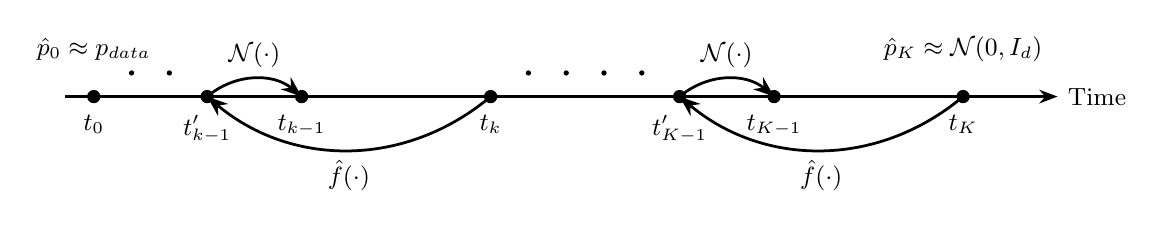
\begin{tikzpicture}[scale=1.2, >=Stealth, 
    thick, % Makes lines and arrows thicker
    every node/.style={font=\small}
  ]

  % Time axis
  \draw[->] (-0.5,0) -- (10,0) node[right] {Time};

  % Points on the time axis
  \node at (-0.2,0.5) {$\hat{p}_0 \approx p_{data}$};
  \fill (-0.2,0) circle (2pt) node[below=3pt] {$t_{0}$};
  \fill (0.2,0.25) circle (0.8pt) node[below=3pt] {};
  \fill (0.6,0.25) circle (0.8pt) node[below=3pt] {};
  \fill (1,0) circle (2pt) node[below=3pt] {$t'_{k-1}$};
  \fill (2,0) circle (2pt) node[below=3pt] {$t_{k-1}$};
  \fill (4,0) circle (2pt) node[below=3pt] {$t_k$};
  \fill (4.4,0.25) circle (0.8pt) node[below=3pt] {};
  \fill (4.8,0.25) circle (0.8pt) node[below=3pt] {};
  \fill (5.2,0.25) circle (0.8pt) node[below=3pt] {};
  \fill (5.6,0.25) circle (0.8pt) node[below=3pt] {};
  \fill (6,0) circle (2pt) node[below=3pt] {$t'_{K-1}$};
  \fill (7,0) circle (2pt) node[below=3pt] {$t_{K-1}$};
  \fill (9,0) circle (2pt) node[below=3pt] {$t_K$};
  \node at (9,0.5) {$\hat{p}_K \approx \mathcal{N}(0,I_d)$};

  % Arrows with increased size and thicker lines
  \draw[->, bend left=40, line width=1pt] (4,0) to node[below] {$\hat{f}(\cdot)$} (1,0); % t_k to t'_{k-1}
  \draw[->, bend left=40, line width=1pt] (1,0) to node[above] {$\mathcal{N}(\cdot)$ } (2,0);
  \draw[->, bend left=40, line width=1pt] (9,0) to node[below] {$\hat{f}(\cdot)$} (6,0); % t_k to t'_{k-1}
  \draw[->, bend left=40, line width=1pt] (6,0) to node[above] {$\mathcal{N}(\cdot )$ } (7,0);
  % t'_{k-1} to t_{k-1}

\end{tikzpicture}
\caption{Demonstrating the step 3 ($\hat{f}$) and 5 ($\mathcal{N}$) of our algorithm w.r.t. the reverse ODE.} 
\label{fig_alg}

\end{figure}




As discussed in the introduction, we consider two analysis based on the assumptions used. In both of our analysis the following assumptiosn are common:

\begin{assumption}
\label{assumption_score_est}
    \textit{The score function estimate} $\{\hat{\vs}_t\}_{1\leq t \leq T}$ obeys for all $t$:
    \begin{equation}
    \label{eq_score_est}
     \mathbb{E}_{\rvx \sim p_{t}}\left [\|\hat{\vs}_{t}(\rvx)- \vs_{t}(\rvx)\|^2 \right ] \leq \varepsilon^2_{score}.
\end{equation}

\end{assumption}

\begin{assumption}
\label{finite_moment}
    The data distribution $p_{data}$ has finite second order moment $\mathbb{E}_{\rvx_0 \sim p_{\text{data}}} \left[ \|\rvx_0\|_2^2 \right] = m_2 < \infty$.
\end{assumption}

\noindent
 Both of these assumptions are pretty standard and have been used in all of the prior works in theoretical analysis of diffusion based generation. We now formalize our setup and discuss the multi-step sampling scheme using consistency models. 

 
\noindent
\begin{algorithm}[H]
\caption{Multi-Step Consistency Generation}
\label{alg:1}
\begin{algorithmic}[1]
\STATE Sample $\hat{\rvx}_K \sim \hat{p}_{t_K}$
\FOR{$k = K, K-1, \ldots, 1$}
    \STATE $\hat{\rvx}'_{k-1} = \hat{f}(t'_{k-1}, t_k, \hat{\rvx}_K)$ \\
    \STATE Sample $z \sim \mathcal{N}(0, I_d)$
    \STATE $\hat{\rvx}_{k-1} = e^{t'_{k-1} - t_{k-1}} \hat{\rvx}'_{k-1} + \sqrt{1 - e^{2(t'_{k-1} - t_{k-1})}}\, z$ 
\ENDFOR
\STATE \textbf{Output} $\hat{\rvx}_0$
\STATE $\hat{p}_{t_0}$ denotes the density of $\hat{\rvx}_0$
\STATE $\hat{p}_{t_0,.., t_K}$ denotes joint density of $(\hat{\rvx}_0, \hat{\rvx}_1, \ldots, \hat{\rvx}_K)$
\end{algorithmic}
\end{algorithm}
\section{Main Results}
\label{sec_3_results}
\noindent
In this section, we provide the theoretical results which advocate for the empirical effectiveness \cite{heek2024multistep} (generating high quality samples in few steps) of the consistency model based formulation. We first provide inference time analysis utilizing the exact consistency function for the empirical PF-ODE (Eq.\ref{empirical_pf_ode}). Then, we provide a theoretical analysis on such consistency functions can be accurately estimated using the consistency distillation training scheme \cite{kim2023consistency}. 
This segregation of training and inference time is done since the usual applications of these diffusion models are majorly concerned with accurate estimation during train time and once trained, are efficient in generation (or inference). Thus, we can train them with arbitrarily small discretization for many steps but for inference only a few steps (and consequently a high discretization complexity) are required for high quality generation.
We now discuss the convergence analysis for the multi-step sampling in Algorithm \ref{alg:1}.

% We first discuss the inference time analysis when
% We will now discuss our convergence results when using the above mentioned formulation of the consistency model.
% We will consider a multi-step sampling approach using these consistency models and show the convergence of the empirical PF ODE to the true data distribution in the KL divergence. We begin by first defining notations/setup followed by stating the assumptions:

% \xh{We may not put all things in this main result chapter.}




% \begin{algorithm}
% \caption{Multi-Step Sampling using Consistency Models.}
% \begin{algorithmic}[1]
% \STATE Sample $\hat{y}_K \sim \hat{p}_{t_K}$
% \FOR{$k = K, K-1, \ldots, 1$}
%     \STATE Let $\hat{y}'_{k-1} = \hat{f}(t'_{k-1}, t_k, \hat{y}_K)$
%     \STATE Let $\hat{y}_{k-1} = e^{t'_{k-1} - t_{k-1}} \hat{y}'_{k-1} + \sqrt{1 - e^{2(t'_{k-1} - t_{k-1})}}\, \epsilon$ \\
%     \hspace{1.1cm} where $\epsilon \sim \mathcal{N}(0, I)$
% \ENDFOR
% \STATE \textbf{Output} $\hat{y}_0$
% \STATE $\hat{p}_{t_0}$ denotes the density of $\hat{y}_0$
% \STATE $\hat{q}$ denotes the joint density of $(\hat{y}_0, \hat{y}_1, \ldots, \hat{y}_K)$
% \end{algorithmic}
% \end{algorithm}

% We consider a sequence $0< t_0 < t_1 < t_2 < \cdots < t_K$ and let $t_j' \in
% [0, t_j)$. Let $\hat{s}_t(\cdot)$ be an approximation of $s_t(\cdot)$, and let
% $\hat{p}_{t_K}$ be an approximation of $p_{t_K}$. 
% % \textbf{Nishant: treat s'=0 for time being}
% \begin{definition}
%   Given $0 \leq s' < s \leq \infty$, and define
%   $\hat{f}(s',s;x)$ be the solution of the following ODE at $t=s'$ 
%   \[
%     d \hat{x}_t = \left(-\hat{x}_t - \hat{s}_t(x_t)\right)dt ,
%   \]
%   with $x_s=x$.
% \end{definition}


% \begin{enumerate}
% \item $\hat{y}_K \sim \hat{p}_{t_K}$ 
% \item For $k=K, K-1,\ldots, 1$
%   \begin{itemize}
%   \item Let $\hat{y}_{k-1}'=\hat{f}(t_{k-1}',t_{k},\hat{y}_K)$
%   \item Let $\hat{y}_{k-1}= e^{t_{k-1}'-t_{k-1}}  \hat{y}_{k-1}' +
%      \sqrt{1-e^{2(t_{k-1}'-t_{k-1})}}  \epsilon$
%     ($\epsilon \sim N(0,I)$)
%   \end{itemize}
% \item Output $\hat{y}_0$. 
% \end{enumerate}

% Let $\hat{p}_{t_0}$ be the density of $\hat{y}_0$.

% Let $\hat{q}$ be the density of $\hat{y}_0,\hat{y}_1,\ldots,\hat{y}_K$. 
% % \textbf{Nishant: log log t steps.}
    
% \vspace{-0.15in}

\subsection{Convergence in the KL divergence for multi-step sampling}
\label{subsec_3_analysis}


\noindent
We first discuss the analysis involving the smoothness of the score function, which has also been widely used in the literature \cite{lyu2024sampling, xu2024provably, chen2022sampling}. The assumption is as follows: 
\begin{assumption}
\label{smoothness_assumption}
    The approximate score function $\hat{\vs}_t$ $L-$Lipschitz with $L\geq 1$ for all $t \geq 1$.
\end{assumption}

\noindent
Notice, that it is a bit different from the previous works \cite{chen2022sampling, xu2024provably, lyu2024sampling, chen2023improved} since they assume the true score to be Lipschitz.
We provide another analysis where we relax this assumption and incur additional dependence on the dimension $d$ replacing $L$. We now provide our first main result as follows.

% \begin{theorem}
% \label{thm:smooth_score_case}
% For  Algorithm~\ref{alg:1}, if $h'_k \leq \frac{1}{2(1+L)}$, $t_k-t'_k=\frac{1}{K}$, where $K$ is the number of iterations and is set to $K\geq 2(L+1)\log\left(\frac{L(d+m_2)}{\varepsilon_{score}}\right)$, along with assumptions \ref{assumption_score_est}, \ref{finite_moment}, \ref{smoothness_assumption}  provided, we have:
%   \[
%    \KL{{p}_{t_0}}{\hat{p}_{t_0}} 
%    \leq {O}\left({\varepsilon^2_{score}}\log^2\left(\frac{L(d+m_2)}{\varepsilon_{score}}\right)\right)  
%  \]

% \end{theorem}
% updated thm 3.1
\begin{theorem}
\label{thm:smooth_score_case}
For  Algorithm~\ref{alg:1}, if $h'_k \leq \frac{1}{2(1+L)}$, along with assumptions \ref{assumption_score_est}, \ref{finite_moment}, \ref{smoothness_assumption}  provided, we have:
  \begin{align}
  \label{smooth_bound_complete_eq}
    KL(p_{t_0}\|\hat{p}_{t_0}) \leq (d+m_2) e^{-T} +  e^{2}{h'}_k^2 \varepsilon^2_{score} \sum_{k=1}^K\frac{1}{4(t_k-t'_k)}
\end{align}

\end{theorem}
\textit{Proof Sketch.}  Please refer Appendix~\ref{appendix:proof_of_thm1} for the complete proof. Here, we discuss a higher level sketch. The proof involves considering the two sources of error: a) Initialization error due to starting the reverse process from a normal distribution (lemma \ref{convergence_of_ou}) and b) the error incurred by using empirical PF ODE (eq. \ref{empirical_pf_ode}) instead of the true PF ODE (eq. \ref{true_pf_ode}, which will depend on $\varepsilon_{score}$). Also, for intuition, the tight control of the KL is due to adding the noise and then re-applying the consistency function $\hat{f}$ in the Algorithm \ref{alg:1} (steps 3 and 5) of the empirical PF-ODE (Eq.\ref{empirical_pf_ode}). 
% \begin{proof}
%     \xh{After demonstrating the theorem, you need to do: (1) provide the place where readers can find the proof. (Appendix~\ref{appendix:proof_of_thm1}) (2) compare the results with previous ones; what kind of improvement have you achieved? (linear vs polynomial complexity) (3) How do you achieve such an improvement? (adding noise in inference cancels the accumulative score estimation error)}
%     The complete proof of this theorem is provided in Appendix~\ref{appendix:proof_of_thm1}. A higher level sketch involves considering the two sources of error: a) Initialization error due to starting the reverse process from a normal distribution (lemma \ref{convergence_of_ou}) and b) the error incurred by using empirical PF ODE (eq. \ref{empirical_pf_ode}) instead of the true PF ODE (eq. \ref{true_pf_ode}, which will depend on $\varepsilon_{score}$). 
    
%     Bounding the first error is straightforward and has been adapted from the existing literature.
% \end{proof}


\noindent
Since we know that the total time of the forward process $T$ would be $\sum^K_{k=1}h_k$, we can conclude the following from this theorem:
\begin{corollary}
 Under Assumptions \ref{assumption_score_est}, \ref{finite_moment}, \ref{smoothness_assumption},   Algorithm \ref{alg:1} achieves the KL divergence error $O(\varepsilon^2)$, if we run it for a total time $T = \log(\frac{d+m_2}{\varepsilon})$
    with the constant step size say $h_k = \frac{1}{3(L+1)}$ and $h'_k = \frac{1}{2(L+1)}$ (which leads to $t_k-t'_k = h'_{k+1}-h_{k+1} = \frac{1}{6(L+1)}$), thereby inducing an iteration/discretization complexity $K=\frac{T}{h_k} = 3(L+1)\log(\frac{d+m_2}{\varepsilon})$ given that the score estimation error from denoising score matching is $\varepsilon_{score} = O\left(\frac{\varepsilon}{\sqrt{log(\frac{d+m_2}{\varepsilon})}}\right)$. 
    
\end{corollary}

\noindent
% \xh{Consider combining this comment with the proof part of Lemma 4.1.}
Therefore, we can have the step size (and correspondingly the number of iterations) independent (logarithmically dependent) of $\varepsilon$ to achieve $O(\varepsilon^2)$ accuracy in the KL divergence which is better then any of the existing results $\left(O(\frac{1}{\epsilon})\right)$ for DDPM \cite{ho2020denoising}/DDIM \cite{song2020denoising} samplers which need step size to be atleast $O(\varepsilon)$ for the SDE based generation \cite{li2024d} (thereby inducing an iteration complexity of $O(\frac{1}{\varepsilon})$) and also require much stricter assumptions for ODE based generation (like the error between Jacobi of true and estimated score is small) \cite{li2024sharp,li2024unified}.
This shows the effectiveness of using the consistency model based formulation for generation tasks with constant step sizes. 
% The best previous works require step size to be atleast $O(\epsilon)$ for the SDE based generation \cite{li2024d} (thereby inducing an iteration complexyt of $O(\frac{1}{\epsilon})$) and require much stricter assumptions for ODE based generation (like the bounded Jacobi) \cite{li2024sharp,li2024unified}. 
Also, we can see that this would not be possible to achieve without multi-step sampling, which requires adding noise at each step into the generated samples. This acts as a regularizer and helps to prevent error accumulation. Intuitively, this is similar to what a stochastic differential equation (SDE) achieves in the score-based formulation. Therefore, it is reasonable to conclude that the theoretical advantages of using consistency models become effective when employing the multi-step iterative sampling approach, while requiring far fewer steps compared to standard diffusion-based generation.

% \noindent
% It might also be possible to study this algorithm further like an SDE and thus have a corresponding Fokker Planck equation. Finding an SDE corresponding to this would be a tricky task and is an interesting future direction to follow up.

\iffalse
%%% comment: I don't feel we have to talk about this here?
\noindent
\paragraph{Limitation.} An issue with this analysis is that we cannot handle the case where the complete sequence $t'_k$ is set to 0 and thereby achieve the theoretical analysis for the original consistency model formulation. This is due to the fact that $h'_k$ has to be bounded, which is required in lemma \ref{main_lemma_smooth} to prove the theorem. This has also been discussed in detail in the Appendix \ref{appendix:proof_of_thm1}. Since TV distance is upper bounded a metric, it might be the case that this can be possible to achieve a TV error of $O(\epsilon)$ by exploiting other tools like fokker planck equation. It can be interesting future direction to follow-up. The other issue the smoothness required for the estimated score function. Since, many recent works \cite{chen2023improved,benton2024nearly} have targetted to relax the requirement of a smooth score function, it can sometimes be treated as non-standard.\\
\fi

\noindent
We now consider relaxing the assumption 3.3 and provide the convergence in KL for the multi-step sampling in the next subsection.

\subsection{The Non-Smooth Case}
\label{non_smooth_subsec}
\noindent
Taking inspiration from recent works \cite{chen2023improved,benton2024nearly} on relaxing the smoothness assumption of the true score function, we first define the noise schedule/conditional variance for $\rvx_t$ given $\rvx_0$ for the forward OU process as $\sigma_t = 1-e^{-2t}$ and arrive at the following result for the multi-step sampling (Algorithm \ref{alg:1}) in absence of any smoothness. 
% \begin{theorem}
% \label{thm:non_smooth_3.3}
%    For Algorithm \ref{alg:1}, using only assumptions \ref{assumption_score_est} and \ref{finite_moment}, if we have $ h'_k < \frac{\sigma^2_{t'_{k-1}}}{d}$ and the number of iterations $K=\frac{d}{\sigma^2_{t'_{k-1}}}\log\left(\frac{(d+m_2)}{\varepsilon_{score}}\right)$, then:
%   \[
%    \KL{{p}_{t_\delta}}{\hat{p}_{t_\delta}} 
%    \leq {O}\left({\varepsilon^2_{score}}\log^2\left(\frac{(d+m_2)}{\varepsilon_{score}}\right)\right) 
%  \]
%  % $t_k-t'_k=O\left(\frac{\sigma^2_{t'_{k-1}}}{d}\right)$
% where $t'_0 = \delta > 0$
% \end{theorem}
\begin{theorem}
\label{thm:non_smooth_3.3}
   For Algorithm \ref{alg:1}, using only assumptions \ref{assumption_score_est} and \ref{finite_moment}, if we have $ {h'}_k < \frac{\sigma^2_{t'_{k-1}}}{d}$ and the number of iterations $K=\frac{d}{\sigma^2_{t'_{k-1}}}\log\left(\frac{(d+m_2)}{\varepsilon_{score}}\right)$, then:
  \begin{align}
KL(p_{t_\delta}\|\hat{p}_{t_\delta}) \leq (d+m_2) e^{-T} +  e^4{h'}_k^2\varepsilon^2_{score} \sum_{k=1}^K\frac{1}{4{(t_k-{t'}_k)}}
  \end{align}
 % $t_k-t'_k=O\left(\frac{\sigma^2_{t'_{k-1}}}{d}\right)$
where $t'_0 = \delta > 0$.
\end{theorem}

\begin{remark}
% \xh{use remark rather than proof, this remark seems good but combines it with Corollary 4.4.}
The proof can be found in the Appendix \ref{appendix_non_smooth}. Again similar to the idea of Theorem \ref{thm:smooth_score_case} proof, we have to consider both initialization error and the error due to empirical ODE (eq. \ref{empirical_pf_ode}). However, since the score function hasn't been provided as smooth here, bounding the error due to the empirical ODE will be a bit more tricky here. Taking inspiration from the previous works, we first try to bound the operator norm of the score function along the true trajectory since, using the fact that the forward process is just a convolution with gaussian distribution and the perturbation can be bounded. 
\end{remark}

\noindent
It is easy to observe that absence of smoothness (the constant $L$) induces a factor of $d$ but the remaining result is similar to the previous theorem and thus, we can again have a similar conclusion as follows.

\begin{corollary}
Under Assumptions \ref{assumption_score_est}, \ref{finite_moment}, Algorithm \ref{alg:1} achieves the KL divergence error $O(\epsilon^2)$, if we run it for a total time $T= \log(\frac{d+m_2}{\epsilon})$
    with the constant step size, say, $h_k = \frac{1-e^{-\delta}}{2d}$ and $h'_k = \frac{1-e^{-\delta}}{d}$, thereby inducing an iteration/discretization complexity $K = \frac{T}{h_k} = \frac{2d}{1-e^{-\delta}}\log(\frac{d+m_2}{\epsilon})$ given that the score estimation error from denoising score matching is $\varepsilon_{score} = O\left(\frac{\epsilon}{\sqrt{\log(\frac{d+m_2}{\epsilon})}}\right)$, better then any of the existing results \cite{benton2023nearly} $\left(O\left(\frac{d}{\epsilon^2}\right)\right)$ for DDPM \cite{ho2020denoising} sampler when the smoothness of the score function is not assumed.
    
\end{corollary}

\noindent
Both this theorem and the previous theorem \ref{thm:smooth_score_case} suffer from the limitation of $h'_k$ being bounded. This limits their applicability to the original consistency model formulation \cite{song2023consistency} which always takes as the end of the reverse flow ODE (or the data distribution)and thus for that the sequence $t'_k$ should be set to 0. This issue has further been discussed in the appendix after the proof of Lemma \ref{main_lemma_smooth}.\\
Seeing the proof of both these theorems, it can be observed that the analysis is almost tight and thus, to resolve this limitation, exploring other metrics like TV distance might be an interesting direction. 
 We now discuss learning the consistency function formulation $\hat{f}$ corresponding to the empirical ODE using the distillation technique proposed in the consistency model paper \cite{song2023consistency}.
 % \xh{Add a table to compare the results with previous ones.}

% We also provide a basic TV analysis in the appendix for this multi-step sampling which results in the similar bounds and doesn't provide any additional gains. However, it is not very tight. Instead discovering the underlying SDE and using a fokker plank based TV analysis \cite{li2024unified} might actually result in more tighter bounds since we are unable to avoid the girsanov's theorem in any of the current analysis. We now discuss learning the consistency function formulation $\hat{f}$ corresponding to the empirical ODE using the distillation technique proposed in the original consistency model paper.

% \subsubsection{Limitations}


\subsection{Consistency Distillation Training to estimate $\hat{f}$}
\label{learning_subsec}

\noindent
In the previous subsection, we discussed how we can exploit the given formulation of the consistency function \textit{i.e.} $\hat{f}(t',t,\rvx_t)$ corresponding to the empirical PF ODE to achieve state of the art convergence results when doing iterative multi-step sampling. However, it is still not clear whether such a consistency function correponding to empirical ODE (eq. \ref{empirical_pf_ode}) can be learned efficiently or not. In this section, we discuss this learning of such consistency function. \\
% \xh{Here we have assumed the consistency function of empirical trajectory exists, but it seems we have not proved it. In other words, is there any function $\hat{f}(t,t^\prime, \cdot)$ can exactly transform the random variable $\hat{\rvx}_t$ to $\hat{\rvx}_{t^\prime}$? Or whether $\hat{\rvx}_t$ and $\hat{\rvx}_{t^\prime}$ can be changed into each other with change of variable?}

\noindent
The original consistency model paper proposes two schemes to learn any consistency function: distillation based training and the self-consistency training. Here, we will consider the first case. It involves using an ODE solver $\Phi$ and distilling its knowledge into the consistency model. Let us denote the parameterized approximation of $\hat{f}$ as $\hat{f}_\theta$. The distillation based training involves considering the true process at $t_{k+1}$: $\rvx_{t_{k+1}} = e^{-t_{k+1}}\rvx_0 + \sqrt{1-e^{-2t_{k+1}}}\epsilon,$ $\epsilon\sim \mathcal{N}(0,I_d)$ and taking one step back to get $\hat{\vx}^\phi_{t_k}$ using a pretrained diffusion model as ODE solver $\phi$ and the empirical PF ODE, denoting this overall one step update as $\Phi(\cdot)$ : 
\begin{align}
\label{update_x}
\hat{\vx}^\phi_{t_k} = \Phi(\rvx_{t_{k+1}},t_{k+1}, t_k) = \rvx_{t_{k+1}} - ({t_{k+1}-t_k}) \hat{s}_{t_{k+1}}(\rvx_{t_{k+1}})
\end{align}
The objective $\mathcal{L}_{CD}$ then is to feed both of these to $\hat{f}_\theta$ and minimize the euclidean distance between the resulting outputs:
\begin{align}
\label{cd_loss}
\mathcal{L}_{\text{CD}}(\theta, \theta^{-}; \Phi) 
:= \mathbb{E}\left[ \lambda(t_n) \left\| \hat{f}_{\theta}(t_0, t_{n+1}, \rvx_{t_{n+1}}) - \hat{f}_{\theta^{-}}(t_0, t_{n}, \hat{\vx}^{\Phi}_{t_n}) \right\|_2^2 \right]
\end{align}
where $\theta^-$is just the running averages of the parameters, done for a stable training and also for faster convergence and $\lambda(\cdot) \in \mathbb{R}^+$ is just a positive weighing function \cite{song2023consistency}. Now, to analyze the difference between true consistency function and the learned consistency function $\hat{f}_\theta$ via the above objective, we first state some assumptions on the training as well as on the parametrized function $\hat{f}_\theta$ itself. These are again standard in literature and have been used the all recent works involving consistency model analysis \cite{kim2023consistency, song2023consistency, lyu2024sampling}.
\\


\noindent
\begin{assumption}
\label{cd_assumption}
    We have the following assumption \cite{song2023consistency, lyu2024sampling} on consistency distillation error for the approximator of $\hat{f}$ \textit{i.e.} $\hat{f}_\theta$:
\begin{equation}
    \mathbb{E}_{\rvx_{t_{k+1}} \sim p_{t_{k+1}}}\left[\|\hat{f}_\theta(t'_{k-1}, t_{k+1}, \rvx_{t_{k+1}}) - \hat{f}_\theta(t'_{k-1}, t_k, \hat{\vx}^\phi_{t_k})\|_2^2\right] 
    \leq \varepsilon^2_\text{cd}(t_{k+1} - t_k)^2, \, \forall \, k \in [1, K - 1],
\end{equation}
\end{assumption}

\begin{assumption}
\label{smooth_f}
    \textit{$\hat{f}_\theta$ is $L_f-$lipschitz} \cite{kim2023consistency, song2023consistency, lyu2024sampling}. \\
\end{assumption}

\noindent
\textbf{Verifying Assumption \ref{smooth_f}.}  Since we have assumed that $\hat{\vs}_t$ is smooth in one of the analysis above, it is straightforward to verify that $\hat{f}(t',t,\cdot)$ would satisfy the following (for intution consider error accumulated in naive euler discretization):
% \xh{how to define $\approx$ between two vector?}
\[
\hat{f}(t', t, x) = 1 + (t - t') + {O}((t - t')^2) \cdot x + \left((t - t') + {O}((t - t')^2)\right) \cdot s_t(x)
\]
% \textcolor{blue}{
% Do you mean the following?
% \[
% \hat{f}(t',t,x) = (1+ (t-t')) x + (t-t') \vs_t(x) + o(t-t').
% \]
% Perhaps we can just write it that way.
% The approximation symbol gives people suspicion.
% }
Abstracting out the higher order $(t-t')$ terms since it is small, we will have:
\begin{align}
\label{approx_smooth_hat_f}
\|\hat{f}(t',t,x)-\hat{f}(t',t,y)\|_2
&\leq \|\left(1+ O(t-t')\right) (x-y)
+ O(t-t') (\hat{\vs}_t(x)-\hat{\vs}_t(y)) \|_2 \notag \\
&\leq \left(1+ O(t-t')\right) \|(x-y) \|_2
+ O(t-t') \|(\hat{\vs}_t(x)-\hat{\vs}_t(y)) \|_2 \notag\\
&\leq
\left(1+(1+L)\cdot O(t-t')\right) \|x-y\|_2  
\end{align}
where $L$ is the Lipschitz of $\hat{\vs}_t$ (Assumption \ref{smoothness_assumption}). For a tight upper bound, we can have:
\[
\|\hat{f}(t',t,x)-\hat{f}(t',t,y)\| \leq 
e^{(1+L)(t-t')} \|x-y\|  
\]
% {Thus, we can set $L_f$ to be $e^{(1+L)(t-t')}$ for $\hat{f}(t',t,\cdot)$.} 
Thus, assuming that $\hat{f}$ would be lipschitz smooth is a reasonable assumption and $L_f$ would be approximately same as $(1+(1+L)(t-t'))$.
Also, we can now directly extend this finding to $\hat{f}_\theta(t',t,x)$ since it should just incur some additional error related to $\varepsilon_{cd}$ which would be of other order $O((t-t')\varepsilon_{cd})$. This will lead to the following:
\[
\| \hat{f}_{\theta}(t'_{n-1}, t_{n}, \vx_{t_n}) - \hat{f}_{\theta}(t'_{n-1}, t_{n}, \vy_{t_n}) \|_2 \leq (t_n - t'_{n-1})(\varepsilon_{\text{cd}}) + L_f \| \vx_{t_n} - \vy_{t_n} \|_2.
\]
Therefore, we can assume that $\hat{f}_\theta(t',t,\cdot)$ would be $L_f$-lipschitz.
% adapt this
% verify and formalize this idea for $\hat{f}_\theta$, we provide, the following lemma from a recent work which shows the Lipschitzness-like property of $\hat{f}_\theta$, assuming that true score ($s_t$) is $L$-Lipschitz. 

% \begin{lemma}[\textbf{Taken from \cite{lyu2024sampling}}]\label{theorem:C.1}
% If we strengthen Assumptions \ref{assumption_score_est} and \ref{cd_assumption} to the \( L_\infty \) norm, that is,
% \begin{equation*}
%     \|\hat{\vs}_{t_n}(x, t_n) - \nabla \vs_{t_n}(x)\|_2 \leq \varepsilon_{\text{sc}}, \quad \forall \, n \in [1, N], \forall x \in \mathbb{R}^d,
% \end{equation*}
% \begin{equation*}
%     \|\hat{f}_{\theta}(0, t_{n+1}, \rvx_{t_{n+1}}) - \hat{f}_{\theta}(0, t_{n+1}, \hat{\vx}^\phi_{ t_n})\|_2 \leq \varepsilon_{\text{cm}} (t_{n+1} - t_n), \quad \forall \, n \in [1, N-1], \quad,
% \end{equation*}
% where
% \begin{equation*}
%     \hat{\vx}^\phi_{t_n} = e^{t_{n+1} - t_n} \vx_{t_{n+1}} + (e^{t_{n+1} - t_n} - 1) \hat{\vs}_{t_{n+1}}(\vx_{t_{n+1}}),
% \end{equation*}
% and if we assume \( p_{\text{data}} \) is $L-$smooth, satisfies Assumption \ref{finite_moment} and is a bounded distribution with radius \( R \), then we have the following statement: There exists \( L_f := e^{C_2 R^2} \) for some \( C_2 > 0 \), such that  
% \begin{equation}
%     \| \hat{f}_{\theta}(0, t_{n}, \vx_{t_n}) - \hat{f}_{\theta}(0, t_{n}, \vy_{t_n}) \|_2 \lesssim (t_n - t_1)(\varepsilon_{\text{cm}} + L_f \varepsilon_{\text{sc}}) + L_f \| \vx_{t_n} - \vy_{t_n} \|_2.
% \end{equation}
% where $\vy_{t_n}$ lie on a (correspond to) different probability flow ODEs (for a given time-stamp $t_n$).
% \end{lemma}
% \begin{proof}
%     For proof, please refer the paper. 
% \end{proof}
% \noindent
% To adapt this to our set-up now, since we have assumed $\hat{s}_t$ smooth instead of $s_t$, we won't have the $\varepsilon_{sc}$ term and thus, for our case it would be:
% \[
% \| \hat{f}_{\theta}(0, t_{n}, \vx_{t_n}) - \hat{f}_{\theta}(0, t_{n}, \vy_{t_n}) \|_2 \lesssim (t_n - t_1)(\varepsilon_{\text{cd}}) + L_f \| \vx_{t_n} - \vy_{t_n} \|_2.
% \]
\noindent
We now provide the following theorem regarding the difference between the estimated consistency function using the distillation based training and true consistency function corresponding to the PF-ODE using the above assumptions.

% \begin{theorem}
% \textbf{(Bounding error between $\hat{f}$ and estimated $f_\theta$ assuming exact consistency distillation)}. Following the definition of $\hat{f}$ from above (def. 3) for some discretization $\{t_n\}_{n\in [1,N]}$ for the consistency distillation training, denoting $\Delta t := \max_{n\in[1,N-1]}\{|t_{n+1} - t_n|\}$, if 
% \[\mathcal{L}_{\text{NCD}}(\theta, \theta; \phi)= \mathbb{E}[\lambda(t_{n-1})d(\hat{f}_\theta(t'_{n-1}, t_{n}, y_k), \hat{f}_\theta(t'_{n-1}, t_{n-1}, y^\phi_{n-1})]  = 0\]
% we have 
% \[ \|\hat{f}_\theta(t'_{n-1}, t_{n}, y_n) - \hat{f}(t'_{n-1}, t_{n}, y_n)\|_2 = \tilde{O}(
% {\underbrace{e^{(1+L)(t_{n-1}-t'_{n-1})}}_{L_f}
% L^{3/2}d^{1/2}}(t_n-t'_{n-1}))\].
% \end{theorem}

\begin{theorem}
\label{thm:gap_f_hat_f_theta}
\textbf{(Bounding error between $\hat{f}$ and estimated $\hat{f}_\theta$)}. Following the definition of $\hat{f}$ for some discretization $\{t_n\}_{n\in [1,N]}$ for the consistency distillation training, 
% denoting $\Delta t := \max_{n\in[1,N-1]}\{|t_{n+1} - t_n|\}$
under assumption 3.1-3.5, we have:
% \[\sup_{n,y} \|\hat{f}_\theta(t'_{n-1}, t_{n}, y_n) - \hat{f}(t'_{n-1}, t_{n}, y_n)\|_2 = \tilde{O}(
% {\underbrace{e^{(1+L)(t_{n-1}-t'_{n-1})}}_{L_f}
% L^{3/2}d^{1/2}}(\Delta t)^2)\].
\begin{align*}
\mathbb{E} \|\hat{f}_\theta(t'_{n-1}, t_{n}, \rvx_n) - \hat{f}(t'_{n-1}, t_{n}, \rvx_n)\|^2_2 \leq  L_fe^{{h_{n-1}}/{2}}(L^{{3}/{2}}d^{{1}/{2}}h_{n-1}) + \varepsilon_{cd}(t_n-t_1).
\end{align*}
\end{theorem}
\begin{proof}
    For proof, please refer to Appendix~\ref{appendix:Thm3_6}.
\end{proof}
\noindent
\textbf{Achieving a good approximation of $\hat{f}$}. Based, on the previous theorem, it is easy to observe that the approximation mainly depends on the consistency distillation training error and the \textit{training time discretization}, both of which can be made arbitrarily small during training and thus, we can argue achieving a very close approximation for $\hat{f}$. Now, we will again consider this approximation analysis but this time when the smoothness assumption on score function is not provided.

\paragraph{Non-smooth case.} We will now consider the scenario where we do not have assumption \ref{smooth_f} where we have shown how to bound the expected value for $\|\nabla \vs_t(\cdot)\|$ on the true trajectory, since if $\hat{\vs}_t$ is not smooth, we cannot verify it and thus, is not a good assumption to have. Here, will use the idea from the proof of theorem \ref{thm:non_smooth_3.3} and will bound the expected difference instead. We can understand this for the true $f$ first as follows for some $\rvx, \rvy \in \mathbb{R}^d$:

\begin{align*}
&\mathbb{E}\|\hat{f}(t',t,\rvx)-\hat{f}(t',t,\rvy)\|_2\\
&\leq \mathbb{E}\|(1+ (t-t')) (\rvx-\rvy)
+ (t-t') (\vs_t(\rvx)-\vs_t(\rvy)) \|_2 \qquad \qquad \qquad\text{(similar argument as Eq. \ref{approx_smooth_hat_f})} \\
&\leq
(t-t') E\|\rvx-\rvy\|_2 + \frac{d}{\sigma_t^2}(t-t') E\left[\|\rvx-\rvy\|_2 \exp\left(\frac{\|\rvx-\rvy\|}{\sigma_t^2}\right)  ,\right] \qquad \text{(Lemma \ref{expected_smooth} Appendix)} \\
&\leq (t-t') E\|\rvx-\rvy\|_2 + \frac{2d}{\sigma_t^2}(t-t') E\|\rvx-\rvy\|_2 \qquad\qquad \qquad \qquad \quad \qquad \text{(when $\rvx,\rvy$ are close)}
\end{align*}



% \noindent
% Now, we provide the following lemma as a counterpart of lemma 3.5 for $\hat{f}_\theta$ in this case: 

% \begin{lemma}[]
% Under assumptions 3.1-3.3 and:
% % \begin{equation}
% %     \|s_{\theta}(x, t_n) - \nabla \log p_{t_n}(x)\|_2 \leq \varepsilon_{\text{sc}}, \quad \forall n \in [[1, N]], \forall x \in \mathbb{R}^d,
% % \end{equation}
% \begin{equation}
%     \|f_{\theta}(0, t_{n+1}, x_{t_{n+1}}) - f_{\theta}(0, t_{n+1}, \hat{x}_{\varphi t_n})\|_2 \leq \varepsilon_{\text{cm}} (t_{n+1} - t_n), \quad \forall n \in [[1, N-1]], \quad x_{t_{n+1}} \in \mathbb{R}^d,
% \end{equation}
% where
% \begin{equation}
%     \hat{x}_{\varphi t_n} = e^{t_{n+1} - t_n} x_{t_{n+1}} + (e^{t_{n+1} - t_n} - 1) s_{\varphi}(x_{t_{n+1}}, t_{n+1}),
% \end{equation}
% and if\( p_{\text{data}} \) is a bounded distribution with radius \( R \), then, there exists \( L_f := e^{C_2 R^2} \) for some \( C_2 > 0 \), such that  
% \begin{equation}
%     E_q\| \hat{f}_{\theta}(0, t_{n}, x_{t_n}) - \hat{f}_{\theta}(0, t_{n}, y_{t_n}) \|_2 \lesssim (t_n - t_1)(\varepsilon_{\text{cm}} + L_f \varepsilon_{\text{sc}}) + L_f \| x_{t_n} - y_{t_n} \|_2.
% \end{equation}
% \end{lemma}
% \begin{lemma}[]
% Under assumptions 3.1-3.4 and using the exponential integrator as the ODE solver during distillation:
% \begin{equation}
%     \hat{x}^\varphi _{t_n} = e^{t_{n+1} - t_n} x_{t_{n+1}} + (e^{t_{n+1} - t_n} - 1) s_{\varphi}(x_{t_{n+1}}, t_{n+1}),
% \end{equation}
% and also assuming \( p_{\text{data}} \) is a bounded distribution with radius \( R \), then, there exists \( L_f := e^{C_2 R^2} \) for some \( C_2 > 0 \), such that  
% \begin{equation}
%     E_q\| \hat{f}_{\theta}(0, t_{n}, x_{t_n}) - \hat{f}_{\theta}(0, t_{n}, y_{t_n}) \|_2 \lesssim (t_n - t_1)(\varepsilon_{\text{cm}} + L_f \varepsilon_{\text{sc}}) + \frac{d^2}{\sigma^2_{t_n}} \| x_{t_n} - y_{t_n} \|_2.
% \end{equation}
% \end{lemma}
\begin{lemma}
\label{lemma_non_smooth_cf_lipschitz}
{(\textbf{Validating the assumption on $\hat{f}_\theta$ in the non-smooth case.})
Using the exponential integrator while the consistency distillation training:
\[
\hat{\vx}^\phi_{t_n} = e^{t_{n+1}-t_n} \rvx_{t_{n+1}} + (e^{t_{n+1}-t_n} - 1) \hat{\vs}_{t_{n+1}}(\rvx_{t_{n+1}}),
\]
and given the assumptions \ref{assumption_score_est}, \ref{finite_moment}, \ref{cd_assumption},  
% along with assuming that $p_{data}$ is a bounded distribution
% % and if we assume $p_{\text{data}}$ satisfies Assumption 3.2, and is a bounded distribution 
% with radius $R$, then there exists $L_f := e^{C_2 R^2}$ for some $C_2 > 0$, such that
we have:
% \[
% \mathbb{E}\|\hat{f}_\theta(0, t_n, \rvx_{t_n}) - \hat{f}_\theta(0, t_n, \rvy_{t_n})\|_2 
% & \leq 2(t_n-t_1)\varepsilon_{cd} + 2C_4\epsilon_{score}d(t_n-t_1) \exp(C_3d) + e^{C_2d}\mathbb{E}\|\rvx_{t_n}-\rvy_{t_n}\|_2 
% \]
\begin{align*}
\mathbb{E}\|f_\theta(t_1, t_n, \rvx_{t_n}) - f_\theta(t_1, t_n, \rvy_{t_n})\|_2 
& \leq 2(t_n-t_1)\varepsilon_{cd} + 2\varepsilon_{score}(t_n-t_1)  + n\mathbb{E}\|\rvx_{t_n}-\rvy_{t_n}\|_2 
\end{align*}
}
\noindent
where again $\vy_{t_n}$ lie on a (correspond to) different probability flow ODEs (for a given time-stamp $t_n$).
\end{lemma}
% \begin{proof}
    % The proof is easy to derive from the proof of lemma 3.7 by taking expectation on both sides and using lemma B.X which bounds the expected value of the hessian. For completeness the proof is provided in the appendix.
\textit{Proof Sketch.} A rough sketch starting from $\hat{\rvx}_{t_n}={\rvx}_{t_n}$ (similarly for ${\rvy}$) and decomposing the terms corresponding to $\rvx, \rvy$ into the additional error aggregation when ${\hat{\rvx}}_{t_{i}}$ is mapped to $t_1$ as against $\hat{\rvx}_{t_{i-1}}$ and similarly for $\rvy$, thereby bounding their difference using the sum of these terms.
% A rough sketch would be similar to the proof of lemma \ref{theorem:C.1} provided in \cite{lyu2024sampling}. 
Also, for this non-smooth scenario, we bound the expectation using our lemma \ref{expected_smooth} by bounding the expected hessian (or gradient of score). Please refer Appendix \ref{appendix:Thm3_6} for the complete proof. It is straightforward to further adapt for any $t'_{n-1}$ as the first parameter as against $t_1$. It has been omitted here for simplicity.
% \end{proof}

\noindent
Now, we again provide the analysis for the approximated consistency model (counterpart of Theorem \ref{thm:gap_f_hat_f_theta}) for the non-smooth case:
\begin{theorem}
\label{3.8thm_gap_f_non_smooth}
Following the definition of $\hat{f}$ for some discretization $\{t_n\}_{n\in [1,N]}$ in the consistency distillation training, 
% denoting $\Delta t := \max_{n\in[1,N-1]}\{|t_{n+1} - t_n|\}$
using assumptions \ref{assumption_score_est}, \ref{finite_moment}, \ref{cd_assumption}, we have:
% \[\sup_{n,y} \|\hat{f}_\theta(t'_{n-1}, t_{n}, y_n) - \hat{f}(t'_{n-1}, t_{n}, y_n)\|_2 = \tilde{O}(
% {\underbrace{e^{(1+L)(t_{n-1}-t'_{n-1})}}_{L_f}
% L^{3/2}d^{1/2}}(\Delta t)^2)\].
% \begin{align*}
%   &\mathbb{E}_{p_{t_1,..,t_K}}\|
%   f(t_{n-1}',t_n,{\rvx}_n)-\hat{f}_\theta(t_{n-1}',t_n,{\rvx}_n)\|_2
%   \leq e^{C_2d}e^{{h_{n-1}}/{2}}(L^{{3}/{2}}d^{{1}/{2}}h_{n-1}) + (t_n-t_1)\left(3\varepsilon_{cd} +2C_4de^{C_3d}\epsilon_{score} \right)
% \end{align*}
\begin{align*}
\E  
  \|
  f(t_{n-1}',t_n,{\rvx}_n)-\hat{f}_\theta(t_{n-1}',t_n,{\rvx}_n)\|_2 \leq ne^{{h_{n-1}}/{2}}(L^{{3}/{2}}d^{{1}/{2}}h_{n-1}) + (t_n-t_1)\left(3\varepsilon_{cd} +2\varepsilon_{score} \right)
\end{align*}

\end{theorem}
% \begin{proof}
   \textit{Proof Sketch.} The proof is similar as Theorem \ref{thm:gap_f_hat_f_theta} but here we instead utilize the Lemma \ref{lemma_non_smooth_cf_lipschitz} and bound the expectation of the term. It incurs a factor of $d$ which arises from the bound on the hessian. Also, here as against Theorem \ref{thm:gap_f_hat_f_theta}, we have bounded the error w.r.t. the true consistency function corresponding to the actual reverse ODE and thus, we incur the additional term involving the score estimation.
    The detailed proof is provided in Appendix \ref{appendix:Thm3_6}. 
% \end{proof}
% \input{0_contents/040analysis}
% \input{0_contents/050exp}
\section{Conclusions}
\noindent
In this work, we provided a theoretical analysis for multi-step generation using consistency models, showing that the number of iterations $K$ (and consequently the step size) for the probability flow ODE based generation  can be independent of $\varepsilon$ to generate samples from a distribution which is $\varepsilon^2-$close in KL divergence to the target distribution, under minimal assumptions. Here, we have achieved $O(d\log(\frac{d}{\varepsilon}))$ convergence which is both \textit{state-of-the-art} w.r.t. to dimension $d$ and also w.r.t. $\varepsilon$ since it has a logarithmic dependence as against $O(\frac{1}{\varepsilon})$ in the current best ODE/SDE based samplers. We also don't require any strict assumptions on Divergence/Jacobi in our ODE based generation as the existing works and even relax the smoothness assumption. 
Furthermore, we also provide a theoretical analysis for estimating the formulation of the consistency function required for our analysis: which can take a point at a given time instant to arbitrary time instants along the reverse probability flow ODE. We show that this can be efficiently estimated using the distillation objective proposed in the original consistency models paper, given we use a fine discretization at the training time. Therefore, it can be concluded from this analysis that estimating accurate consistency function and combining them with iterative generation scheme involving noise addition can lead to much faster generation theoretically as against the typical DDPM typle samplers. An interesting future direction might be to further loosen the bound on step size to accomodate original consistency model formulation and maybe achieve tigher theoretical guarantees.



\bibliographystyle{apalike}
\bibliography{0_contents/ref}  %%% Uncomment this line and comment out the ``thebibliography'' section below to use the external .bib file (using bibtex) .


%%% Uncomment this section and comment out the \bibliography{references} line above to use inline references.
% \begin{thebibliography}{1}

% 	\bibitem{kour2014real}
% 	George Kour and Raid Saabne.
% 	\newblock Real-time segmentation of on-line handwritten arabic script.
% 	\newblock In {\em Frontiers in Handwriting Recognition (ICFHR), 2014 14th
% 			International Conference on}, pages 417--422. IEEE, 2014.

% 	\bibitem{kour2014fast}
% 	George Kour and Raid Saabne.
% 	\newblock Fast classification of handwritten on-line arabic characters.
% 	\newblock In {\em Soft Computing and Pattern Recognition (SoCPaR), 2014 6th
% 			International Conference of}, pages 312--318. IEEE, 2014.

% 	\bibitem{hadash2018estimate}
% 	Guy Hadash, Einat Kermany, Boaz Carmeli, Ofer Lavi, George Kour, and Alon
% 	Jacovi.
% 	\newblock Estimate and replace: A novel approach to integrating deep neural
% 	networks with existing applications.
% 	\newblock {\em arXiv preprint arXiv:1804.09028}, 2018.

% \end{thebibliography}

\newpage
\tableofcontents
\newpage

\newpage
\appendix
% \section{Technical Appendices and Supplementary Material}

\section{Actual counterpart of our algorithm}
As discussed in the paper, below we provide the true counterpart of our multi-step consistency sampling Algorithm \ref{alg:1} which involves using the true consistency function $f$ as against $\hat{f}$ and thereby leads us to the true distribution. Note, since it is using the true consistency function, it follows the true distribution $p_{t_1,...,t_K}$ as against the $\hat{p}_{t_1,...,t_K}$ and can also be treated as a \textit{True Reverse Process}.
\noindent
\begin{algorithm}[H]
\caption{Multi-Step Consistency Generation}
\label{alg:2}
\begin{algorithmic}[1]
\STATE Sample ${\rvx}_K \sim {p}_{t_K}$
\FOR{$k = K, K-1, \ldots, 1$}
    \STATE ${\rvx}'_{k-1} = {f}(t'_{k-1}, t_k, {\rvx}_K)$ \\
    \STATE Sample $z \sim \mathcal{N}(0, I_d)$
    \STATE ${\rvx}_{k-1} = e^{t'_{k-1} - t_{k-1}} {\rvx}'_{k-1} + \sqrt{1 - e^{2(t'_{k-1} - t_{k-1})}}\, z$ 
\ENDFOR
\STATE \textbf{Output} ${\rvx}_0$
\STATE ${p}_{t_0}$ denotes the density of ${\rvx}_0$
\STATE ${p}_{t_0,.., t_K}$ denotes joint density of $({\rvx}_0, {\rvx}_1, \ldots, {\rvx}_K)$
\end{algorithmic}
\end{algorithm}

\section{Proof of Theorem~\ref{thm:smooth_score_case}}

\label{appendix:proof_of_thm1}
\noindent


% \textcolor{blue}{\hrule \hfill}

\noindent
Here, we provide the proof of our first main result. As highlighted in the high-level proof in the main paper, we bound the two errors: the error due to empirical PF ODE
and the initialization error. We first discuss bounding the former below.

\subsection{Error due to the empirical PF ODE (eq. \ref{empirical_pf_ode}).} 
\label{err_1}
As discussed in the algorithms provided in the main, we will denote the joint distribution of the true and approximate process by $p_{t_1, t_2, ..., t_{K}}$ and $\hat{p}_{t_1, t_2, ..., t_{K}}$ respectively. The overall idea is to bound the KL between the outputs using the data processing inequality and bounding the KL between $\hat{p}_{t_1, t_2, ..., t_{K}}$ and $p_{t_1, t_2, ..., t_{K}}$ which can be done by rewriting them using transition (conditional) probabilities. The following two lemmas describe this idea. \\

\noindent
\textbf{Notational Remark.} As discussed in the Subsection \ref{subsec_3_notations} of the main paper, we will use the notations $\rvx_{t_k}$ and $\rvx_{k}$ interchangeably both corresponding to true (resp. empirical) PF ODE at time $t_k$ (resp. $t'_{k-1}$) for a given sequence $\{t_k\}$ (resp. $\{t'_k\}$).

\vspace{0.2in}

\begin{lemma}
\label{lemma_first_kl_bw_conditionals}
 Denoting $\hat{p}_{k-1|k}$ be the conditional probability of
  $\hat{\rvx}_{k-1}$  given $\hat{\rvx}_k$, and let
  ${p}_{k-1|k}$ be the conditional probability of
  $\rvx_{k-1}$ given $\rvx_k$. Then
  \[
    \KL{{p}_{k-1|k}(\cdot|{\rvx}_{k})}{\hat{p}_{k-1|k}(\cdot|{\rvx}_k)}
    =  e^{2(t_{k-1}'-t_{k-1})}
    \frac{\|
      f(t_{k-1}',t_k,{\rvx}_k)-\hat{f}(t_{k-1}',t_k, {\rvx}_k)\|_2^2}
    {2 (1  -e^{2(t_{k-1}'-t_{k-1})})}     
  \]
\end{lemma}
\begin{proof}
For this, we know that from Algorithm~\ref{alg:2} that the conditional ${p}_{k-1|k}(\cdot|{\rvx}_{k})$ is the following Gaussain: \[
{p}_{k-1|k}(\cdot|{\rvx}_{k}) \sim \mathcal{N}\left(e^{t_{k-1}' - t_{k-1}} f(t_{k-1}', t_k, \rvx_k), \left(1 - e^{2(t_{k-1}' - t_{k-1})}\right) I_d \right)
\]
where $I_d$ is the d-dimensional identity matrix. Similarly, from Algorithm \ref{alg:1}:
\[
\hat{p}_{k-1|k}(\cdot|{\rvx}_{k}) \sim \mathcal{N}\left(e^{t_{k-1}' - t_{k-1}} \hat{f}(t_{k-1}', t_k, \rvx_k), \left(1 - e^{2(t_{k-1}' - t_{k-1})}\right) I_d \right)
\]
Now, since the covariance matrices are same for both, we can just use the following formulae for calculating KL between two gaussians with different means but same variance:
\[
\KL{{p}_{k-1|k}(\cdot|{\rvx}_{k})}{{p}_{k-1|k}(\cdot|{\rvx}_k)} = \frac{1}{2}(\mu_1-\mu_2)^T\sum(\mu_1-\mu_2)  
\]
where $\mu_1$, $\mu_2$ corresponds to the mean of the two distributions and $\sum$ corresponds to their covariance. For this case, we have:
\begin{align*}
\mu_1 &= e^{t_{k-1}' - t_{k-1}} f(t_{k-1}', t_k, \rvx_k) \\
\mu_2 &= e^{t_{k-1}' - t_{k-1}} \hat{f}(t_{k-1}', t_k, \rvx_k) \\
\Sigma &= \left(1 - e^{2(t_{k-1}' - t_{k-1})} \right) I_d
\end{align*}
Merely substituting these values in the KL formulae will lead to the desired term. \\
\end{proof}


\noindent
We will now utilize this expression to bound the KL between outputs of Algorithms \ref{alg:1} and \ref{alg:2} using the following lemma:

\vspace{0.2in}
\begin{lemma}
\label{lemma_second_KL_data_processing_ineq}
  We have
  \begin{align*}
    \KL{{p}_{t_0}}{\hat{p}_{t_0}}
    \leq & \KL{{p}_{t_1, t_2, ..., t_{K}}}{\hat{p}_{t_1, t_2, ..., t_{K}}}\\
    =& \KL{{p}_{t_K}}{\hat{p}_{t_K}} + 
   \E_{{p}_{t_1,..,t_{K}}} \left[ \sum_{k=1}^K
       \KL{{p}_{k-1|k}(\cdot|{\rvx}_{k})}{\hat{p}_{k-1|k}(\cdot|{\rvx}_k)}\right]
  \end{align*}
\end{lemma}
\begin{proof}
Since we know that LHS corresponds to first marginalizing the corresponding joint distributions and then calculating KL and RHS is the KL div between the joint distributions. Using data processing inequality, it is straightforward to argue that the inequality holds. The second equation is just decomposing the KL of the joint distribution into conditionals which can be easily verified by merely writing the RHS expression using the KL formulae. 
\end{proof}

\noindent
We now provide another lemma which will be useful in relating the expected difference between the true and approximate process generated from empirical PF ODE with the corresponding consistency functions.


\vspace{0.2in}
\begin{lemma}
\label{change_of_var_lemma}
    Given deterministic functions $g$ and $\hat{g}$ on a random variable $\rvy$ and also given random variables $\rvx,\hat{\rvx}$
 such that $\rvx=g(\rvy)$ and $\hat{\rvx}=\hat{g}(\rvy)$, then we have:
 \[
 \mathbb{E}_{\rvx,\hat{\rvx}}\|\rvx-\hat{\rvx}\|^2 = \mathbb{E}_{\rvy}\|g(\rvy)-\hat{g}(\rvy)\|^2
 \]
 \end{lemma}
 \begin{proof}
     We can write expectation of a deterministic function of random variables: 
     \[
     \mathbb{E}_{\rvx,\hat{\rvx}}[h(\rvx,\hat{\rvx}] = \int\int h(\rvx,\hat{\rvx})f_{\rvx,\hat{\rvx}}(\vx,\hat{\vx})d\vx d\hat{\vx}
     \]
     where $f_{\rvx,\hat{\rvx}}$ is the joint distribution of the two random variables. Now, since we know that $\rvx$, $\hat{\rvx}$ are not independent and each correspond to a deterministic function of some random variable $\rvy$ where $\rvx=g(\rvy)$ and $\hat{\rvx}=\hat{g}(\rvy)$. Thus, if we know $\rvy$, we have the value of $\rvx$, $\hat{\rvx}$ fixed and thus, we can use the change of variables in the previous expression:
     \[
     \mathbb{E}_{\rvx,\hat{\rvx}}[h(\vx,\hat{\vx})] = \int\int h(\vx,\hat{\vx})f_{\rvx,\hat{\rvx}}(\vx,\hat{\vx})d\vx d\hat{\vx} = \int h(g(\vy),\hat{g}(\vy))f_\rvy(\vy)d\vy = \mathbb{E}_\rvy[ h(g(\vy),\hat{g}(\vy))]
     \]
     where $f_\rvy$ is the distribution of $\rvy$ given $h$ is measurable. Now, using the choice of $h$ as $\|\cdot \|^2$, which satisfies the requirement, leads to our result. 
 \end{proof}
%  \begin{proof}
%      We have:
%      \begin{align*}
%          \int_{(x,\hat{x})} p({x,\hat{x}}) \cdot\|x-\hat{x}\|^2 d (x, \hat{x}) &= \int_{x,\hat{x}} \left(\int_y p(y)\cdot p(x,\hat{x}|y) dy \right) \cdot \|x-\hat{x}\|^2 d(x,\hat{x}) \\
%          &= \int_y p(y)\int_{x,\hat{x}}p(x,\hat{x}|y)\cdot\|x-\hat{x}\|^2 d(x,\hat{x}) dy \\
%          &= \int_y p(y) \left(g(y) - \hat{g}(y)\right)
%      \end{align*}
% since given $y$, $x$ and $\hat{x}$ are deterministic \xh{the last step is confusing why it has
% \begin{equation*}
%     \int_{x,\hat{x}}p(x,\hat{x}|y)\cdot\|x-\hat{x}\|^2 d(x,\hat{x}) = \|g(y) - \hat{g}(y)\| ?
% \end{equation*}
% please use the standard method (change of variable) to prove this result.}
%  \end{proof}

\vspace{0.2in}
\noindent
We now provide our most important lemma for this proof, which bounds the numerator in the RHS in Lemma \ref{lemma_first_kl_bw_conditionals} based on Young's inequality and Gronwall's inequality.

\begin{lemma}
\label{main_lemma_smooth}
  For any $\delta>0$ with $\varepsilon_{score} = O(\delta)$, we can choose $t'_{k-1}$ such that $h'_k=t_{k}-t'_{k-1}  \leq \frac{1}{2(1+L)}$, and discretization 
$h_{k-1} = t_{k}-t_{k-1} < \frac{1}{2(1+L)}$ (since $t'_{k-1}<t_{k-1}$ thus $h_k$<$h'_k$) and have:
\[
  \E_{{p}_{t_1,.., t_{K}}}  
  \|
  f(t_{k-1}',t_k,{\rvx}_k)-\hat{f}(t_{k-1}',t_k,{\rvx}_k)\|_2^2 \leq e^2({h'}_k^2\varepsilon^2_{score}) = {O}\left( \frac{ \varepsilon^2_{score}}{L^2}\right) = 
  {O}(\delta^2) .
\]
\end{lemma}
\begin{proof}
Given the definition of $f(\cdot)$ and $\hat{f}(\cdot)$ above that these correspond to the solutions of actual ODE (eq. \ref{true_pf_ode}) and empirical ODE at $t=t'_{k-1}$ (eq. \ref{empirical_pf_ode}), we have:
\begin{equation*}
    f(t_{k-1}^\prime, t_k, \rvx_k) = \rvx_{t_{k-1}^\prime},  \quad \hat{f}(t_{k-1}',t_k,{\rvx}_k) = \hat{\rvx}_{t^\prime_{k-1}}
\end{equation*}
Now, since $f$ and $\hat{f}$ are deterministic mappings being applied to $\rvy_k$ here, using Lemma \ref{change_of_var_lemma}, we can just rewrite this as:

\begin{equation*}
    \begin{aligned}
        &\E_{\rvx_k \sim {p}_{t_1,.., t_{K}}}\left\|f(t_{k-1}',t_k,{\rvx}_k)-\hat{f}(t_{k-1}',t_k,{\rvx}_k)\right\|^2 = \E_{\rvx_{t^\prime_{k-1}}, \hat{\rvx}_{t^\prime_{k-1}}}\left\|\rvx_{t^\prime_{k-1}} - \hat{\rvx}_{t^\prime_{k-1}} \right\|^2 
    \end{aligned}
\end{equation*}
Now, to bound this, we use $\Delta_t$ to denote the difference between $x_t$ and $\hat{x}_t$: $\Delta_t=\rvx_t-\hat{\rvx}_t$. Then, we have:
\begin{equation*}
\begin{aligned}
    \frac{d \|\Delta_t\|^2}{dt} = 2\langle\Delta_t, \frac{d \Delta_t}{dt}\rangle &= 2\|\Delta_t\|^2 + 2\langle\Delta_t,s_t(x_t)-\hat{s}_t(\hat{x}_t)\rangle \\
    &\leq 2\|\Delta_t\|^2 + 2\|\Delta_t\|\|s_t(\rvx_t)-\hat{s}_t(\hat{\rvx}_t)\| \\
    &\leq 2\|\Delta_t\|^2 + 2\|\Delta_t\|\left(\|\hat{\vs}_t(\rvx_t)-\hat{\vs}_t(\hat{\rvx}_t)\| +\|\vs_t({x}_t)-\hat{\vs}_t({\rvx}_t)\|\right) \\
    &\leq (2+2L)\|\Delta_t\|^2 + 2\|\Delta_t\|\left(\|\vs_t({\rvx}_t)-\hat{\vs}_t({\rvx}_t)\|\right) \\
    &\leq \left(2+2L+\frac{1}{h'_k}\right) \|\Delta_t\|^2 + h'_k\|\vs_t({\rvx}_t)-\hat{\vs}_t({\rvx}_t)\|^2 \qquad \text{(Young's Inequality)}
    \end{aligned}
\end{equation*}
where $h'_k = t_k-t'_{k-1}$ Now, using Gronwall's inequality, we have:
\begin{align*}
\mathbb{E}\left[\left\| \rvx_{t'_{k-1}} - \hat{\rvx}_{t'_{k-1}} \right\|^2\right] &\leq \exp\left(\left(2 + 2L +  \frac{1}{h'_k} \right)h'_k\right)\left(  \int_{t'_{k-1}}^{t_k}  h'_{k}\, \mathbb{E}\left[\left\|   \vs_t({\rvx}_t) - \hat{\vs}_{t}({\rvx}_{t}) \right\|^2\right] dt \right) \\
& \leq \exp\left(\left(2 + 2L +  \frac{1}{h'_k} \right)h'_k\right)\left(  \int_{t'_{k-1}}^{t_k}  h'_{k}\, \varepsilon^2_{score} dt \right) \quad \text{(using Assumption \ref{assumption_score_est})} \\
% &\quad \leq h'_k \int_{t'_{k-1}}^{t_k} \mathbb{E}\left[\left\|   s_t(x_t) - \hat{s}_{t}(\hat{x}_{t}) \right\|^2\right] dt \approx h'^2_k \mathbb{E}\left[\left\|   s_{t'_{k-1}}(x_{t'_{k-1}}) - \hat{s}_{t'_{k-1}}(\hat{x}_{t'_{k-1}}) \right\|^2\right]
&= \exp\left(\left(2 + 2L +  \frac{1}{h'_k} \right)h'_k\right)\left(    h'^2_{k}\, \varepsilon^2_{score} \right) \quad \\
\end{align*}
The exponential part is given by:
\[
\exp\left(\left(2 + 2L + \frac{1}{h_k'}\right) h_k'\right) = \exp\left(2h_k' + 2Lh_k' + \frac{h_k'}{h_k'}\right) = \exp\left(h_k'( 2 + 2L) + 1\right).
\]
For large \( L \), the dominant term in the exponential is \( 2Lh_k' \). If \( h_k' \) does not decay sufficiently with \( L \), this term grows very rapidly. Thus, we need to control the first term in the exponential by constraining $h'_k < \frac{1}{2(1+L)}$ resulting in the overall term of the order ${O}(\frac{\varepsilon^2_{score}}{L^2})$ and we have the following final expression:

\begin{align}
     \E_{{p}_{t_1,.., t_{K}}}  
  \|
  f(t_{k-1}',t_k,{\rvx}_k)-\hat{f}(t_{k-1}',t_k,{\rvx}_k)\|_2^2 < e^2({h'}_k^2\varepsilon^2_{score})
\end{align}

\end{proof}

\noindent
\textit{\textbf{Setting} $\{t'_k\} = 0$} \textit{\textbf{to replicate the original consistency models?}} A possibility of setting the sequence $t'_k=0$ is there but then $h'_k < \frac{1}{2(1+L)}$ is not guaranteed and for this, we can just instead use $h'_k={O}(\log(1/\delta))$ but then $\varepsilon_{score}={O}(\frac{\delta^{L+1.5}}{\sqrt{log(1/\delta)}})$, where $L\geq 1$, which would thus require a very accurate estimation of score as against $\tilde{O}(L\delta)$ before. Thus, as highlighted in the main paper its adaptation to the original consistency model formulation is not straightforward.\\

\noindent
\subsection{Initialization Error.} 
\label{appendix_init_error}
If we define the forward noising process for a total time $T$ (and consequently $K$ total iterations where $\sum_{k=0}^K h_k + t_0= T$), we know that the $p_T={law}(\rvx_T)$ is still not exactly $\mathcal{N}(0,I_d)$ and is just close to it. So when we initialize the reverse/generation process with gaussian, this leads to the initialization error which is the difference between the distribution after running the forward process on the original data distribution for time $T$ and the standard gaussian distribution, which can be bounded as follows: \\



\begin{lemma}
\label{convergence_of_ou}
    (\textbf{Convergence of the OU process}). Under Assumption \ref{finite_moment}, for \( T > 1 \), we have
\[
KL(p_T \parallel \gamma_d) \leq (d + m_2) e^{-T}.
\]
where $T$ is the total time for the forward process and $m_2 = \mathbb{E}_{p_t}[\|\vx\|_2^2]$.
% OU process started with $q^{\to}_{0} = q^\star$ where $q^\to_t$ denotes the marginal at $t$. 
\end{lemma}
\begin{proof}
For any \( t > 0 \), we can use Jensen’s inequality to bound the entropy of \( p_t \):

\begin{align*}
    \int_{\mathbb{R}^d} p_t(\vx) \log p_t(\vx) \, d\vx &= \int_{\mathbb{R}^d} \left( \int_{\mathbb{R}^d} p_{t|0}(\vx|\vx_0) dP(\vx_0) \right) \log \left( \int_{\mathbb{R}^d} p_{t|0}(\vx|\vx_0) dP(\vx_0) \right) d\vx \\
&\leq \int_{\mathbb{R}^d} \left( \int_{\mathbb{R}^d} p_{t|0}(\vx|\vx_0) \log p_{t|0}(\vx|\vx_0) dP(\vx_0) \right) d\vx \\
& = \int_{\mathbb{R}^d} \left( \int_{\mathbb{R}^d} p_{t|0}(\vx|\vx_0) \log p_{t|0}(\vx|\vx_0) d\vx \right) dP(\vx_0). \\
\end{align*}

\noindent
Since for the considered OU proces, we have  \( \rvx_t | \rvx_0 \sim \mathcal{N}(\alpha_t x_0, \sigma_t^2 I_d) \), where $\sigma_t^2=1-e^{-t}$, we have
\[
\int_{\mathbb{R}^d} p_{t|0}(\vx|\vx_0) \log p_{t|0}(\vx|\vx_0) \, d\vx = -\frac{d}{2} \log(2\pi \sigma_t^2) - \frac{d}{2}.
\]
Thus,
\[
\int_{\mathbb{R}^d} p_t(\vx) \log p_t(\vx) \, d\vx \leq -\frac{d}{2} \log(2\pi \sigma_t^2) - \frac{d}{2}.
\]
Therefore,
\[
KL(p_t \parallel \gamma_d) = \int_{\mathbb{R}^d} p_t(\vx) \log p_t(\vx) \, d\vx + \mathbb{E}_{p_t} \left[ \|\vx\|^2_2 + \frac{d}{2} \log(2\pi) \right]
\leq \frac{d}{2} \log \sigma_t^{-2} + \frac{1}{2} (m_2 - d).
\]
From the exponential convergence of Langevin dynamics with a strongly log-concave stationary distribution, we obtain
\[
KL(p_T \parallel \gamma_d) \leq e^{-T + t} \left( \frac{d}{2} \log \sigma_t^{-2} + \frac{1}{2} (m_2 - d) \right).
\]
By choosing \( t = \log 2 \), we have
\[
e^t \log \left( \frac{1}{\sigma_t^2} \right) \leq 1.
\]
Thus,
\[
KL(p_T \parallel \gamma_d) \leq e^{-T} (d + m_2).
\]
\end{proof}

\noindent
\subsection{Proving Theorem \ref{thm:smooth_score_case}.} 
\label{proving_thm_3.1}
Given the above lemmas corresponding to the error components, we now provide the proof for Theorem 3.3 as follows:
\begin{proof}
From {Lemma \ref{lemma_second_KL_data_processing_ineq}}, we have:
% \[
% \mathrm{KL}(p_{t_0} \| \hat{p}_{t_0}) \leq \mathrm{KL}(q \| \hat{q}) = \mathrm{KL}(p_{t_K} \| \hat{p}_{t_K}) + \mathbb{E}_q \left[ \sum_{k=1}^K \mathrm{KL}(q_{k-1,k}(\cdot|y_k) \| \hat{q}_{k-1,k}(\cdot|y_k)) \right].
% \]
\begin{align*}
    \KL{{p}_{t_0}}{\hat{p}_{t_0}}
    \leq & \KL{{p}_{t_1, t_2, ..., t_{K}}}{\hat{p}_{t_1, t_2, ..., t_{K}}}\\
    =& \KL{{p}_{t_K}}{\hat{p}_{t_K}} + 
   \E_{{p}_{t_1,..,t_{K}}} \left[ \sum_{k=1}^K
       \KL{{p}_{k-1|k}(\cdot|{\rvx}_{k})}{\hat{p}_{k-1|k}(\cdot|{\rvx}_k)}\right]
\end{align*}

\noindent
From {Lemma \ref{lemma_first_kl_bw_conditionals}}, the conditional KL divergence between ${p}_{k-1|k}$ and $\hat{p}_{k-1|k}$ is given by:
% \[
% \mathrm{KL}(q_{k-1,k}(\cdot|y_k) \| \hat{q}_{k-1,k}(\cdot|y_k)) = \frac{e^{2(t_k' - t_k)}}{2(1 - e^{2(t_k' - t_k)})} \| f(t_k', t_k, y_k) - \hat{f}(t_k', t_k, y_k) \|_2^2.
% \]
\[
    \KL{{p}_{k-1|k}(\cdot|{\rvx}_{k})}{\hat{p}_{k-1|k}(\cdot|{\rvx}_k)}
    =  e^{2(t_{k-1}'-t_{k-1})}
    \frac{\|
      f(t_{k-1}',t_k,{\rvx}_k)-\hat{f}(t_{k-1}',t_k, {\rvx}_k)\|_2^2}
    {2 (1  -e^{2(t_{k-1}'-t_{k-1})})}     
  \]
Substituting this into the sum in {Lemma \ref{lemma_second_KL_data_processing_ineq}}, we get:
\[
% \mathbb{E}_q \left[ \sum_{k=1}^K \mathrm{KL}(q_{k-1,k} \| \hat{q}_{k-1,k}) \right] 
\E_{{p}_{t_1,..,t_{K}}} \left[ \sum_{k=1}^K
       \KL{{p}_{k-1|k}(\cdot|{\rvx}_{k})}{\hat{p}_{k-1|k}(\cdot|{\rvx}_k)}\right] = 
\sum_{k=1}^K \frac{e^{2(t_k' - t_k)}}{2(1 - e^{2(t_k' - t_k)})} \mathbb{E}_{{p}_{t_1,..,t_{K}}} \| f(t_k', t_k, \rvx_k) - \hat{f}(t_k', t_k, \rvx_k) \|_2^2.
\]
From {Lemma \ref{main_lemma_smooth}}, we know:
% \[
% \mathbb{E}_q \| f(t_k', t_k, y_k) - \hat{f}(t_k', t_k, y_k) \|_2^2 = \tilde{O}(\frac{\varepsilon^2_{score}}{L^2}) = O(\delta^2),
% \]
\[
  \E_{{p}_{t_1,.., t_{K}}}  
  \|
  f(t_{k-1}',t_k,{\rvx}_k)-\hat{f}(t_{k-1}',t_k,{\rvx}_k)\|_2^2  < e^2({h'}_k^2\varepsilon_{score}) =  {O}\left( \frac{ \varepsilon^2_{score}}{L^2}\right) 
\]
when $h_k < h'_k < \frac{1}{2(L+1)}$. Let us denote the upper bound on this term as $Q =e^{2}{h'}_k^2\varepsilon_{score}^2$ for all $k$.  Therefore, we now have:
\[
% \mathbb{E}_q \left[ \sum_{k=1}^K \mathrm{KL}(q_{k-1,k} \| \hat{q}_{k-1,k}) \right] 
E_{{p}_{t_1,..,t_{K}}} \left[ \sum_{k=1}^K
       \KL{{p}_{k-1|k}(\cdot|{\rvx}_{k})}{\hat{p}_{k-1|k}(\cdot|{\rvx}_k)}\right]\leq  Q \sum_{k=1}^K\frac{e^{-2(t_k-t'_k)}}{2(1-e^{-2(t_k-t'_k)})}
\]
\end{proof}




\noindent
\textbf{Bounding $KL({p}_{t_K}\|\hat{p}_{t_K})$}. Assuming that we start from a normal distribution as an approximateand taking $h_k=\tilde{O}(1/L)$, after running for $K=TL$ iterations (with $T$ being the total time) using {Lemma \ref{convergence_of_ou}}, we have:
\[
KL(\hat{p}_{t_K}\|p_{t_K}) = KL(p_{t_K}\|\gamma^d) \leq ({d}+m_2) \text{exp}(-T)
\]
Therefore, now have the following bound:
\[
KL(p_{t_0}\|\hat{p}_{t_0}) \leq (d+m_2) e^{-T} +  Q \sum_{k=1}^K\frac{e^{-2(t_k-t'_k)}}{2(1-e^{-2(t_k-t'_k)})} \leq (d+m_2) e^{-T} +  Q \sum_{k=1}^K\frac{1}{4(t_k-t'_k)}
\]
where the last inequality uses the fact $e^x\geq 1+x$ after multiplying the numerator and denominator with $e^{2(t_k-t'_k)}$. Substituting the value of $Q$ ow we have:
\begin{align*}
    KL(p_{t_0}\|\hat{p}_{t_0}) \leq (d+m_2) e^{-T} +  e^2{h'}_k^2\varepsilon^2_{score} \sum_{k=1}^K\frac{1}{4(t_k-t'_k)}
\end{align*}
Now choosing $K=2(L+1)\log\left(\frac{L(d+m_2)}{\varepsilon_{score}}\right)$, $t_k-t'_k = \frac{1}{K}$, we have: 
\[
KL(p_{t_0}\|\hat{p}_{t_0}) \leq {O}\left(\frac{\varepsilon^2_{score}}{L^2}\cdot K^2\right) = {O}\left({\varepsilon^2_{score}}\log^2\left(\frac{L(d+m_2)}{\varepsilon_{score}}\right)\right)
\]

\vspace{0.2in}
\section{ Proof of theorem \ref{thm:non_smooth_3.3}}
\label{appendix_non_smooth}
\noindent
The proof in this part also similar to the proof in the previous section, however, since we do not have an assumption on the smoothness of the score function, we need to find an alternate way to control the $\|\vs_t(\rvx_t)-{\vs}_t(\hat{\rvx}_t)\|^2$ term in Lemma \ref{main_lemma_smooth}. For this, we take inspiration from literature \cite{chen2023improved,benton2024nearly} on SDE based diffusion analysis which analyses in the absence of smoothness assumptions. We begin by first providing a lemma adapted from \cite{chen2023improved} that bounds the Gaussian perturbation of a given probability distribution in $d-$dimension as follows. 

\subsection{Error due to empirical PF-ODE (Eq. \ref{empirical_pf_ode}): Non-smooth case}
\label{error_due_to_empirical_non_smooth}

\begin{lemma}
\label{adapted_from_improved}
\textbf{(Taken from \cite{chen2023improved})}. Let $P$ be a probability measure on $\mathbb{R}^d$. Consider the density of its Gaussian perturbation
\[
p_\sigma(\vx) \propto \int_{\mathbb{R}^d} \exp \left(- \frac{\|\vx - \vy\|^2}{2\sigma^2} \right) dP(\vy).
\]
Then for $\rvx \sim p_\sigma$, we have the sub-exponential norm bound
\[
\|\nabla^2 \log p_\sigma(\rvx)\|_{F, \psi_1} \leq \frac{d}{\sigma^2},
\]
where $\| \cdot \|_{F, \psi_1} = \| \| \cdot \|_F \|_{\psi_1}$ denotes the sub-exponential norm of the Frobenius norm of a random matrix.
\end{lemma}

\begin{proof}
We just provide a sketch here for reference. For the detailed proof please refer Lemma 12 in \cite{chen2023improved}.
First, we will have the following equation for conditional density
$\tilde{P}_\sigma(\vy|\vx)$:
\[
d\tilde{P}_\sigma(\vy|\vx) \propto \exp \left(- \frac{\|\vy - \vx\|^2}{2\sigma^2} \right) dP(\vy).
\]
Now, just writing $\nabla^2 \log p_\sigma$ in terms of $\operatorname{Var}_{\tilde{P}_\sigma(\vy|\vx)} \left( \frac{\vy}{\sigma^2} \right)$ and using the following inequality for any integer $q$:
\[
\mathbb{E}_{p_\sigma(\vx)} \left[ \| \operatorname{Var}_{\tilde{P}_\sigma(\vy|\vx)} ( \vy / \sigma^2 ) \|_F^q \right] \leq \frac{1}{\sigma^{2p}} \mathbb{E}_{p_\sigma(x)} \left[ \mathbb{E}_{\tilde{P}_\sigma(\vy|\vx)} \| (\vy - \vx)/\sigma (\vy - \vx)/\sigma^\top \|_F^q \right].
\]
and using the fact that $\frac{\rvy-\rvx}{\sigma}$ is normally distributed, we can derive the result.


% \[
% \nabla^2 \log p_\sigma(\vx) = \operatorname{Var}_{\tilde{P}_\sigma(\vy|\vx)} \left( \frac{\vy}{\sigma^2} \right) - \frac{I_d}{\sigma^2}.
% \]
% For any positive integer $p$, using the fact that $\frac{\rvy-\rvx}{\sigma}$ is distributed as $\mathcal{N}(0, I_d)$ and the power mean inequality,
% \[
% \mathbb{E}_{p_\sigma(\vx)} \left[ \| \operatorname{Var}_{\tilde{P}_\sigma(\vy|\vx)} ( \vy / \sigma^2 ) \|_F^p \right] \leq \frac{1}{\sigma^{2p}} \mathbb{E}_{p_\sigma(x)} \left[ \mathbb{E}_{\tilde{P}_\sigma(\vy|\vx)} \| (\vy - \vx)/\sigma (\vy - \vx)/\sigma^\top \|_F^p \right].
% \]
% Since $z \sim \mathcal{N}(0, I_d)$, we obtain
% \[
% \mathbb{E}_{z \sim \mathcal{N}(0, I_d)} \| zz^\top \|_F^p \lesssim \left( \frac{pd}{\sigma^2} \right)^p.
% \]
% Using the arbitrariness of $p$, we conclude that
% \[
% \| \operatorname{Var}_{\tilde{P}_\sigma(\vy|\vx)} ( \vy / \sigma^2 ) \|_{F, \psi_1} \lesssim \frac{d}{\sigma^2}.
% \]
% Thus, by the triangle inequality,
% \[
% \| \nabla^2 \log p_\sigma(\vx) \|_{F, \psi_1} \lesssim \frac{d}{\sigma^2}.
% \]
% This completes the proof. \\
\end{proof}

\noindent
We now use the above lemma to bound the expectation of our target term $\|\vs_t(\rvx_t)-{\vs}_t(\hat{\rvx}_t)\|^2$ and provide the following lemma.

\begin{lemma}
\label{expected_smooth}
 We have:
 \begin{equation}
     \mathbb{E}\|s_t(\rvx_t)-s_t(\hat{\rvx}_t)\|^2 \leq \frac{d^2}{\sigma_t^4}\mathbb{E}\left[ \|\Delta_t\|^2\exp\left(\frac{\|\Delta_t\|^2}{2\sigma_t^2}\right) \right]
     % \mathbb{E}\left(\frac{d\Delta_t}{\sigma_t^2}\right)^2 \mathbb{E}\exp\left(\frac{\|\Delta_t\|^2}{2\sigma_t^2}\right) 
     % \leq O(\frac{d^2 \|\Delta_t\|^2}{\sigma_t^4})
 \end{equation}
 where $\Delta_t = \rvx_t-\hat{\rvx}_t$ as defined above.
\end{lemma}
\begin{proof}
    We can bound the difference using the hessian as follows:
    \[
        \vs_t(\vx_t) - {\vs}_t(\hat{\vx}_t) = \int_{0}^1 \nabla \vs_t(\vx_t+a(\hat{\vx}_t-\vx_t))(\hat{\vx}_t-\vx_t)da
    \]
    Thus, we would have:
    \[
   \mathbb{E} \|\vs_t(\rvx_t)-\vs_t(\hat{\rvx}_t)\|^2 \leq \int_{0}^1 \mathbb{E}\|\nabla \vs_t(\rvx_t+a\Delta_t)\Delta_t\|^2da
    \]


    \noindent
    Bounding the term inside the integral in the RHS using change of measure we have:
    \begin{align*}
    \mathbb{E}\|\nabla \vs_t(\rvx_t+a\Delta_t)\Delta_t\|^2 &= \mathbb{E}\left[\|\nabla \vs_t(\rvx_t)\Delta_t\|^2 \frac{d P_{\rvx_t+a\Delta_t,\Delta_t}(\rvx_t,\Delta_t)}{d P_{x_t,\Delta_t}(\rvx_t,\Delta_t)} \right] \\
    % &\lesssim \left( \underbrace{\mathbb{E}\|\nabla s_t(x_t) \Delta_t\|^4}_{T_1} \underbrace{\mathbb{E}\left( \frac{d P_{x_t+a\Delta_t,\Delta_t}(x_t,\Delta_t)}{d P_{x_t,\Delta_t}(x_t,\Delta_t)} \right)^2}_{T_2}  \right)^{1/2}
    &\leq \left( \underbrace{\mathbb{E}\|\nabla \vs_t(\rvx_t)\|^4}_{T_1} \underbrace{\mathbb{E}\left( \|\Delta_t\|^2\frac{d P_{\rvx_t+a\Delta_t,\Delta_t}(\rvx_t,\Delta_t)}{d P_{\rvx_t,\Delta_t}(\rvx_t,\Delta_t)} \right)^2}_{T_2}  \right)^{1/2}
    \end{align*}
% \textbf{Bounding $T_1$:} We have: $\|\nabla s_t(x_t)\Delta_t\|_2 \leq \|\nabla s_t(x_t)\|_F\|\Delta_t\|_2 \lesssim \frac{d}{\sigma^2_t}\|\Delta_t\|$ using lemma 3.7. Therefore, we can now bound $T_1$ as:
% \[
% T_1 \lesssim \mathbb{E}\left(\frac{d\Delta_t}{\sigma_t^2}\right)^4 
% \]
\textbf{Bounding $T_1$:} Using Lemma \ref{adapted_from_improved}. Therefore, we can now bound $T_1$ as:
\[
T_1 \leq \mathbb{E}\left(\frac{d}{\sigma_t^2}\right)^4  = \left(\frac{d}{\sigma_t^2}\right)^4
\]
\textbf{Bounding $T_2$:} We have using the data processing inequality:
\begin{align*}
    \mathbb{E}\left( \frac{d P_{\rvx_t+a\Delta_t,\Delta_t}(\rvx_t,\Delta_t)}{d P_{\rvx_t,\Delta_t}(\rvx_t,\Delta_t)} \right)^2 &= \mathbb{E}\left( \frac{d P_{\rvx_t+a\Delta_t|\Delta_t}(\rvx_t|\Delta_t)}{d P_{\rvx_t|\Delta_t}(\rvx_t|\Delta_t)} \right)^2 \\
    &\leq  \mathbb{E}\left( \frac{d P_{\rvx_t+a\Delta_t|\Delta_t,\rvx_0}(\rvx_t|\Delta_t,\rvx_0)}{d P_{\rvx_t|\Delta_t,\rvx_0}(\rvx_t|\Delta_t,\rvx_0)} \right)^2 \\
    &= \mathbb{E}\left( \frac{d P_{\rvx_t+a\Delta_t|\Delta_t,\rvx_0}(\rvx_t|\Delta_t,\rvx_0)}{d P_{\rvx_t|\rvx_0}(\rvx_t|,\rvx_0)} \right)^2
\end{align*}
Therefore, we will have:
\[
\mathbb{E}\left( \|\Delta_t\|^2 \frac{d P_{\rvx_t+a\Delta_t,\Delta_t}(\rvx_t,\Delta_t)}{d P_{\rvx_t,\Delta_t}(\rvx_t,\Delta_t)} \right)^2 \leq \mathbb{E}\left( \|\Delta_t\|^2 \frac{d P_{\rvx_t+a\Delta_t|\Delta_t,\rvx_0}(\rvx_t|\Delta_t,\rvx_0)}{d P_{\rvx_t|\rvx_0}(\rvx_t|,\rvx_0)} \right)^2
\]
Now we know that $\rvx_t+a\Delta_t|(\Delta_t,\rvx_0)\sim \mathcal{N}(\alpha_t^{-1}\rvx_0+a\Delta_t,\sigma_t^2)$ and $\rvx_t|\rvx_0\sim \mathcal{N}(\alpha_t^{-1}\rvx_0,\sigma_t^2I_d)$. Therefore, we have:
\[
\mathbb{E}\left( \|\Delta_t\|^2\frac{d P_{\rvx_t+a\Delta_t|\Delta_t,\rvx_0}(\rvx_t|\Delta_t,\rvx_0)}{d P_{\rvx_t|\rvx_0}(\rvx_t|,\rvx_0)} \right) = \mathbb{E}\left[\|\Delta_t\|^2\exp\left(\frac{a^2\|\Delta_t\|^2}{2\sigma_t^2}\right)\right] 
% \leq \mathbb{E}\exp\left(\frac{\|\Delta_t\|^2}{\sigma_t^2}\right) 
\]
% Therefore, we have:
% \begin{align*}
% \mathbb{E}\|\nabla s_t(x_t+a\Delta_t)\Delta_t\|^2 &\leq \mathbb{E}\left(\frac{d\Delta_t}{\sigma_t^2}\right)^2 \mathbb{E}\exp\left(\frac{a^2\|\Delta_t\|^2}{2\sigma_t^2}\right) \\
% &\leq \mathbb{E}\left(\frac{d\Delta_t}{\sigma_t^2}\right)^2 \mathbb{E}\exp\left(\frac{a\|\Delta_t\|^2}{2\sigma_t^2}\right)
% \end{align*}
Therefore, we have:
\begin{align*}
\mathbb{E}\|\nabla s_t(_t+a\Delta_t)\Delta_t\|^2 &\leq \left(\frac{d}{\sigma_t^2}\right)^2 \mathbb{E}\left[\|\Delta_t\|^2\exp\left(\frac{a^2\|\Delta_t\|^2}{2\sigma_t^2}\right)\right]\\
& \leq \left(\frac{d}{\sigma_t^2}\right)^2 \mathbb{E}\left[\|\Delta_t\|^2\exp\left(\frac{\|\Delta_t\|^2}{2\sigma_t^2}\right)\right]
\end{align*}
Now integrating $a$ from $0$ to $1$ gives the desired result. \\
\end{proof}

\noindent
We will now provide a version of Lemma \ref{main_lemma_smooth} which doesn't require smoothness assumption on the score function. Here, we will use the previous lemma to instead bound the target term. \\


\begin{lemma}
\label{main_lemma_non_smooth}
   For any $\delta>0$ with $\varepsilon_{score} = O(\delta)$, we can choose $t'_{k-1}$ such that $h'_k=t_{k}-t'_{k-1}  < \frac{1}{d^2}$, and consequently discretization 
$h_{k} = t_{k}-t_{k-1} < \frac{1}{d^2}$ (since $t'_{k-1}<t_{k-1}$ thus $h_k$<$h'_k$) and have:
\[
  \E_{p_{t_1,...,t_K}}  
  \|
  f(t_{k-1}',t_k,{\rvx}_k)-\hat{f}(t_{k-1}',t_k,{\rvx}_k)\|_2^2  \leq e^4{h'}_k^2\varepsilon^2_{score} 
  % \tilde{O}(d^2 \sigma_{t'_{k-1}}^2 h'^3_k \varepsilon_{{score}}^2)  = 
  % \tilde{O}\left( { \sigma_{t'_{k-1}}^2 h'_k^2\varepsilon^2_{score}}\right)
  % % = \tilde{O}\left( { \sigma_{t'_{k-1}}^2 \varepsilon^2_{score}}\right) = 
  % {O}(\delta^2) .
\]
\end{lemma}
\begin{proof}
Similar to proof of Lemma \ref{main_lemma_smooth} we begin with:
\begin{equation*}
    f(t_{k-1}^\prime, t_k, \rvx_k) = \vx_{t_{k-1}^\prime},  \hat{f}(t_{k-1}',t_k,{\rvx}_k) = \hat{\vx}_{t^\prime_{k-1}}
\end{equation*}
Now, since $f$ and $\hat{f}$ are deterministic mappings being applied to $\rvy_k$ here, using {Lemma \ref{change_of_var_lemma}}, we can just rewrite this as:

\begin{equation*}
    \begin{aligned}
        &\E_{\rvx_k \sim {p}_{t_1,.., t_{K}}}\left\|f(t_{k-1}',t_k,{\rvx}_k)-\hat{f}(t_{k-1}',t_k,{\rvx}_k)\right\|^2 = \E_{\rvx_{t^\prime_{k-1}}, \hat{\rvx}_{t^\prime_{k-1}}}\left\|\rvx_{t^\prime_{k-1}} - \hat{\rvx}_{t^\prime_{k-1}} \right\|^2 
    \end{aligned}
\end{equation*}
Now, to bound this, we use $\Delta_t$ to denote the difference between $x_t$ and $\hat{x}_t$: $\Delta_t=x_t-\hat{x}_t$. Then, we have the following differential equation based on the evolution of $\rvx_t$ and $\hat{\rvx}_t$:
\[
\frac{d \|\Delta_t\|^2}{dt} = 2\langle\Delta_t, \frac{d \Delta_t}{dt}\rangle = 2\|\Delta_t\|^2 + 2\langle\Delta_t,\vs_t(\rvx_t)-\hat{\vs}_t(\hat{\rvx}_t)\rangle \\
\]
Taking expecation w.r.t. $\rvx_k$ and then using Lemma \ref{change_of_var_lemma}, we have:
\begin{equation*}
\begin{aligned}
\mathbb{E}_{\rvx_k} \frac{d \|\Delta_t\|^2}{dt}  = \frac{d \mathbb{E}_{\rvx_k}\|\Delta_t\|^2}{dt}  &= 2\mathbb{E}_{\rvx_k}\|\Delta_t\|^2 + 2\mathbb{E}_{\rvx_k}\langle\Delta_t,\vs_t(\rvx_t)-\hat{\vs}_t(\hat{\rvx}_t)\rangle \\
    \end{aligned}
\end{equation*}


\noindent
Using Lemma \ref{change_of_var_lemma}, this can be further written as:
\begin{equation*}
\begin{aligned}
&\mathbb{E}_{\rvx_k}\frac{d \|\Delta_t\|^2}{dt} \\
&= 2\mathbb{E}\|\Delta_t\|^2 + 2\mathbb{E}\langle\Delta_t,\vs_t(\rvx_t)-\hat{\vs}_t(\hat{\rvx}_t)\rangle \\
    &\leq 2\mathbb{E}\|\Delta_t\|^2 + 2\mathbb{E}\left[\|\Delta_t\|\|\vs_t(\rvx_t)-\hat{\vs}_t(\hat{\rvx}_t)\| \right] \\
    &\leq 2\mathbb{E}\|\Delta_t\|^2 + 2\mathbb{E}\left[\|\Delta_t\|\left(\|\vs_t(\rvx_t)-{\vs}_t(\hat{\rvx}_t)\| +\|\vs_t(\hat{\rvx}_t)-\hat{\vs}_t(\hat{\rvx}_t)\|\right) \right]\\
    &\leq (2+\frac{1}{h'_k})\mathbb{E}\|\Delta_t\|^2 + 2\mathbb{E}\left[\|\Delta_t\|\left(\|\vs_t(\hat{\rvx}_t)-\hat{\vs}_t(\hat{\rvx}_t)\|\right)\right] + \mathbb{E}\left[\|\vs_t(\rvx_t)-{\vs}_t(\hat{\rvx}_t)\|^2\right] \qquad \text{(Young's Inequality)} \\
    &\leq (2+\frac{1}{h'_k} + \frac{1}{h'_k})\mathbb{E}\|\Delta_t\|^2 + h'_k\mathbb{E}\left[\|\vs_t(\hat{\rvx}_t)-\hat{\vs}_t(\hat{\rvx}_t)\|^2\right] + \mathbb{E}\left[\|\vs_t(\rvx_t)-{\vs}_t(\hat{\rvx}_t)\|^2\right] \qquad \text{(Young's Inequality)} \\
    &\leq \left(2+\frac{1}{h'_k}+\frac{1}{h'_k}\right)\mathbb{E} \|\Delta_t\|^2 + h'_k\mathbb{E}\|\vs_t(\hat{\rvx}_t)-\hat{\vs}_t(\hat{\rvx}_t)\|^2 + \frac{d^2h'_k}{\sigma_t^4}\mathbb{E}\left[\|\Delta_t\|^2\exp\left(\frac{\|\Delta_t\|^2}{2\sigma_t^2}\right) \right] \qquad \text{(Lemma \ref{expected_smooth})}\\
    &\leq \left(2+\frac{1}{h'_k}+\frac{1}{h'_k}\right)\mathbb{E} \|\Delta_t\|^2 + h'_k\varepsilon^2_{score} + \frac{d^2h'_k}{\sigma_t^4}\mathbb{E}\left[\|\Delta_t\|^2\exp\left(\frac{\|\Delta_t\|^2}{2\sigma_t^2}\right) \right] \qquad \qquad  \qquad\text{(Assumption \ref{assumption_score_est})}\\
    &=  \left(2+\frac{1}{h'_k}+\frac{1}{h'_k}\right)\mathbb{E} \|\Delta_t\|^2 + h'_k\varepsilon^2_{score} + \frac{d^2h'_k}{\sigma_t^4}\mathbb{E}\left[\|\Delta_t\|^2 \right]+ \frac{d^2h'_k}{\sigma_t^4}\mathbb{E}\left[\|\Delta_t\|^2\left(\exp\left(\frac{\|\Delta_t\|^2}{2\sigma_t^2}\right) -1 \right)\right]\\
    &\leq \left(2+\frac{1}{h'_k}+\frac{1}{h'_k}\right)\mathbb{E} \|\Delta_t\|^2 + h'_k\varepsilon^2_{score} + \frac{2d^2h'_k}{\sigma_t^4}\mathbb{E}\left[\|\Delta_t\|^2 \right]\\
    \end{aligned}
\end{equation*}

\noindent
where $h'_k = t_k-t'_{k-1}$. Now, applying Gronwall's inequality will result in:

\begin{align*}
\mathbb{E}\left[\left\| x_{t'_{k-1}} - \hat{x}_{t'_{k-1}} \right\|^2\right]
& \leq \exp\left(\left(2 + \frac{2d^2h'_k}{\sigma_{t'_{k-1}}^4} +  \frac{2}{h'_k} \right)h'_k\right)\left(  \int_{t'_{k-1}}^{t_k}  h'_{k}\, \varepsilon^2_{score} dt \right) \quad  \\
% &\quad \leq h'_k \int_{t'_{k-1}}^{t_k} \mathbb{E}\left[\left\|   s_t(x_t) - \hat{s}_{t}(\hat{x}_{t}) \right\|^2\right] dt \approx h'^2_k \mathbb{E}\left[\left\|   s_{t'_{k-1}}(x_{t'_{k-1}}) - \hat{s}_{t'_{k-1}}(\hat{x}_{t'_{k-1}}) \right\|^2\right]
&\leq \exp\left(\left(2 + \frac{2d^2h'_k}{\sigma_{t'_{k-1}}^4} +  \frac{2}{h'_k} \right)h'_k\right)\left(    h'^2_{k}\, \varepsilon^2_{score} \right) \quad \\
\end{align*}
The exponential part is given by:
\[
 \exp\left(\left(2 + \frac{2d^2h'_k}{\sigma_{t'_{k-1}}^4} +  \frac{2}{h'_k} \right)h'_k\right) = \exp\left(2h_k' +  \frac{2d^2h'^2_k}{\sigma_{t'_{k-1}}^4} + 2\right).
\]
For large \( d \), the dominant term in the exponential is \( \frac{2d^2h'^2_k}{\sigma_{t'_{k-1}}^4} \). If \( h'^2_k \) does not decay sufficiently with \(\frac{d^2}{\sigma_{t'_{k-1}}^4} \), this term grows very rapidly. Thus, we need to control the first term in the exponential by constraining $h'_k < \frac{\sigma_{t'_{k-1}}^2}{d}$ resulting in
\begin{align}
    \E_{p_{t_1,...,t_K}}  
  \|
  f(t_{k-1}',t_k,{\rvx}_k)-\hat{f}(t_{k-1}',t_k,{\rvx}_k)\|_2^2 \leq e^4 {h'}_k^2\varepsilon^2_{score}
\end{align}
and thus,  the overall term is of the order ${O}(\frac{\sigma_{t'_{k-1}}^4\varepsilon^2_{score}}{d^2})$. \\


\end{proof}





\subsection{Proving Theorem \ref{thm:non_smooth_3.3}} 
\label{proving_thm_3.3}
Now, using the above lemmas we provide the proof of the Theorem \ref{thm:non_smooth_3.3}, which is quite similar in structure to Theorem \ref{thm:smooth_score_case} proof discussed in the previous section. 

% For reference we provide the theorem again below followed by its proof.


% \begin{theorem}
%   (\textbf{Theorem 3.5}) For algorithm 1, using only assumptions 3.1 and 3.2, if we have $h'_k = t_k-t'_{k-1} < \frac{\sigma^2_{t'_{k-1}}}{d}$, $t_k-t'_k=O\left(\frac{\sigma^2_{t'_{k-1}}}{d}\right)$ and the number of iterations $K=\tilde{O}\left(\frac{d}{\sigma^2_{t'_{k-1}}}\log\left(\frac{(d+m_2)}{\varepsilon_{score}}\right)\right)$, then:
%   \[
%    \KL{{p}_{t_\delta}}{\hat{p}_{t_\delta}} 
%    \leq \tilde{O}\left({\varepsilon^2_{score}}\log^2\left(\frac{(d+m_2)}{\varepsilon_{score}}\right)\right) 
%  \]
% where $t_\delta > t'_0 = \delta > 0$
% \end{theorem}

\begin{proof}
% From \textbf{Lemma A.2}, we have:
% \[
% \mathrm{KL}(p_{t_\delta} \| \hat{p}_{t_\delta}) \leq \mathrm{KL}(q \| \hat{q}) = \mathrm{KL}(p_{t_K} \| \hat{p}_{t_K}) + \mathbb{E}_q \left[ \sum_{k=1}^K \mathrm{KL}(q_{k-1,k}(\cdot|y_k) \| \hat{q}_{k-1,k}(\cdot|y_k)) \right].
% \]
% % Here:
% % \begin{itemize}
% %     \item $\mathrm{KL}(p_{t_K} \| \hat{p}_{t_K})$ quantifies the initial divergence between $p_{t_K}$ and $\hat{p}_{t_K}$.
% %     \item $\mathbb{E}_q \left[ \sum_{k=1}^K \mathrm{KL}(q_{k-1,k} \| \hat{q}_{k-1,k}) \right]$ captures the cumulative error in the backward process.
% % \end{itemize}
% % To show that $\mathrm{KL}(p_{t_0} \| \hat{p}_{t_0}) = \tilde{O}(\delta)$, we must bound these terms. \\

% \noindent
% From \textbf{Lemma A.1}, the conditional KL divergence between $q_{k-1,k}$ and $\hat{q}_{k-1,k}$ is given by:
% \[
% \mathrm{KL}(q_{k-1,k}(\cdot|y_k) \| \hat{q}_{k-1,k}(\cdot|y_k)) = \frac{e^{2(t_k' - t_k)}}{2(1 - e^{2(t_k' - t_k)})} \| f(t_k', t_k, y_k) - \hat{f}(t_k', t_k, y_k) \|_2^2.
% \]
% Substituting this into the sum in \textbf{Lemma A.2}, we get:
% \[
% \mathbb{E}_q \left[ \sum_{k=1}^K \mathrm{KL}(q_{k-1,k} \| \hat{q}_{k-1,k}) \right] = \sum_{k=1}^K \frac{e^{2(t_k' - t_k)}}{2(1 - e^{2(t_k' - t_k)})} \mathbb{E}_q \| f(t_k', t_k, y_k) - \hat{f}(t_k', t_k, y_k) \|_2^2.
% \]
From {Lemma \ref{lemma_second_KL_data_processing_ineq}}, we have:
% \[
% \mathrm{KL}(p_{t_0} \| \hat{p}_{t_0}) \leq \mathrm{KL}(q \| \hat{q}) = \mathrm{KL}(p_{t_K} \| \hat{p}_{t_K}) + \mathbb{E}_q \left[ \sum_{k=1}^K \mathrm{KL}(q_{k-1,k}(\cdot|y_k) \| \hat{q}_{k-1,k}(\cdot|y_k)) \right].
% \]
\begin{align*}
    \KL{{p}_{t_0}}{\hat{p}_{t_0}}
    \leq & \KL{{p}_{t_1, t_2, ..., t_{K}}}{\hat{p}_{t_1, t_2, ..., t_{K}}}\\
    =& \KL{{p}_{t_K}}{\hat{p}_{t_K}} + 
   \E_{{p}_{t_1,..,t_{K}}} \left[ \sum_{k=1}^K
       \KL{{p}_{k-1|k}(\cdot|{\rvx}_{k})}{\hat{p}_{k-1|k}(\cdot|{\rvx}_k)}\right]
\end{align*}

\noindent
From {Lemma \ref{lemma_first_kl_bw_conditionals}}, the conditional KL divergence between ${p}_{k-1|k}$ and $\hat{p}_{k-1|k}$ is given by:
% \[
% \mathrm{KL}(q_{k-1,k}(\cdot|y_k) \| \hat{q}_{k-1,k}(\cdot|y_k)) = \frac{e^{2(t_k' - t_k)}}{2(1 - e^{2(t_k' - t_k)})} \| f(t_k', t_k, y_k) - \hat{f}(t_k', t_k, y_k) \|_2^2.
% \]
\[
    \KL{{p}_{k-1|k}(\cdot|{\rvx}_{k})}{\hat{p}_{k-1|k}(\cdot|{\rvx}_k)}
    =  e^{2(t_{k-1}'-t_{k-1})}
    \frac{\|
      f(t_{k-1}',t_k,{\rvx}_k)-\hat{f}(t_{k-1}',t_k, {\rvx}_k)\|_2^2}
    {2 (1  -e^{2(t_{k-1}'-t_{k-1})})}     
  \]
Substituting this into the sum in {Lemma \ref{lemma_second_KL_data_processing_ineq}}, we get:
\[
% \mathbb{E}_q \left[ \sum_{k=1}^K \mathrm{KL}(q_{k-1,k} \| \hat{q}_{k-1,k}) \right] 
\E_{{p}_{t_1,..,t_{K}}} \left[ \sum_{k=1}^K
       \KL{{p}_{k-1|k}(\cdot|{\rvx}_{k})}{\hat{p}_{k-1|k}(\cdot|{\rvx}_k)}\right] = 
\sum_{k=1}^K \frac{e^{2(t_k' - t_k)}}{2(1 - e^{2(t_k' - t_k)})} \mathbb{E}_{{p}_{t_1,..,t_{K}}} \| f(t_k', t_k, \rvx_k) - \hat{f}(t_k', t_k, \rvx_k) \|_2^2.
\]
From {Lemma \ref{main_lemma_non_smooth}} , we know that for $t'_k\geq\delta>0$:
% \[
% \E_{{p}_{t_1,.., t_{K}}}  
%   \|
%   f(t_{k-1}',t_k,{\rvx}_k)-\hat{f}(t_{k-1}',t_k,{\rvx}_k)\|_2^2 = \tilde{O}({\sigma_{t'_{k-1}}^2\varepsilon^2_{score}h'^3_kd^2})
% \]
\[
\E_{{p}_{t_1,.., t_{K}}}  
  \|
  f(t_{k-1}',t_k,{\rvx}_k)-\hat{f}(t_{k-1}',t_k,{\rvx}_k)\|_2^2 \leq e^4{h'}_k^2\varepsilon^2_{score} = O\left({\frac{\varepsilon^2_{score}\sigma^4_{t'_{k-1}}}{d^2}}{}\right)
\]
 when $h_k < h'_k < \frac{\sigma^2_{t'_{k-1}}}{d}$. Let us denote the upper bound on this term as $Q=e^4{h'}_k^2\varepsilon^2_{score}$ for all $k$. \\
Therefore, we now have:
\[
% \mathbb{E}_q \left[ \sum_{k=1}^K \mathrm{KL}(q_{k-1,k} \| \hat{q}_{k-1,k}) \right]
E_{{p}_{t_1,..,t_{K}}} \left[ \sum_{k=1}^K
       \KL{{p}_{k-1|k}(\cdot|{\rvx}_{k})}{\hat{p}_{k-1|k}(\cdot|{\rvx}_k)}\right]
\leq  Q \sum_{k=1}^K\frac{e^{-2(t_k-t'_k)}}{2(1-e^{-2(t_k-t'_k)})}
\]


% \noindent
% Choosing $t_k' - t_k = O(1/K)$, we can bound the scaling factor $\frac{e^{2(t_k' - t_k)}}{1 - e^{2(t_k' - t_k)}}$ as $O(K)$ (\textit{via taylor's expansion}). Thus:
% \[
% \mathbb{E}_q \left[ \sum_{k=1}^K \mathrm{KL}(q_{k-1,k} \| \hat{q}_{k-1,k}) \right] = \tilde{O}(\frac{K^2 \varepsilon^2_{score}}{L^2}) = O(\delta^2).
% \]
% % \subsection*{Step 3: Bounding $\mathrm{KL}(p_{t_K} \| \hat{p}_{t_K})$}
% where we use the assumption $K=O(1)$ provided in the theorem. \\

\noindent
\textbf{Bounding $KL(\hat{p}_{t_K}\|p_{t_K})$}. Assuming that we start from a normal distribution as an approximate, after running for $K=\frac{1}{h_k}$, where $h_k=t_k-t_{k-1}$ iterations (with $T$ being the total time), using {Lemma \ref{convergence_of_ou}}, we have:
\[
KL(\hat{p}_{t_K}\|p_{t_K}) = KL(p_{t_K}\|\gamma^d) \leq ({d}+m_2) \text{exp}(-T)
\]
Therefore, now have the following bound:
\[
KL(p_{t_\delta}\|\hat{p}_{t_\delta}) \leq (d+m_2) e^{-T} +  Q \sum_{k=1}^K\frac{e^{-2(t_k-t'_k)}}{2(1-e^{-2(t_k-t'_k)})} \leq (d+m_2) e^{-T} +  Q \sum_{k=1}^K\frac{1}{4{(t_k-t'_k)}}
\]
where the last inequality uses the fact $e^x\geq 1+x$ after multiplying the numerator and denominator with $e^{2(t_k-t'_k)}$. Substituting $Q$ results in:
\begin{align*}
    KL(p_{t_\delta}\|\hat{p}_{t_\delta}) \leq (d+m_2) e^{-T} +  e^4{h'}_k^2\varepsilon^2_{score} \sum_{k=1}^K\frac{1}{4{(t_k-t'_k)}}
\end{align*}
Now choosing $K=\frac{1}{h_k}\log\left(\frac{(d+m_2)}{\varepsilon^2_{score}}\right)$, where $h_k = t_k-t_{k-1}$,  and thereby $T=\log\left(\frac{(d+m_2)}{\varepsilon^2_{score}}\right)$, we have: 
\[
KL(p_{t_\delta}\|\hat{p}_{t_\delta}) \leq (d+m_2) e^{-T} +  KQ \cdot O\left(\frac{1}{t_k-t'_k} \right) \leq (d+m_2) e^{-T} +  O\left({{\frac{\varepsilon^2_{score}\sigma^4_{t'_{k-1}}}{d^2}}{}}\cdot \frac{1}{h_k} \cdot \frac{1}{t_k-t'_k}\right) 
\]
Since $h_k<h'_k$, we can substitute $h_k = O\left(\frac{\sigma^2_{t'_{k-1}}}{d}\right)$ and similarly we can also substitute $t_k-t'_k=O\left(\frac{\sigma^2_{t'_{k-1}}}{d}\right)$ it finally reduces to:
\[
KL(p_{t_\delta}\|\hat{p}_{t_\delta}) \leq {O}\left({\varepsilon^2_{score}}\log\left(\frac{(d+m_2)}{\varepsilon^2_{score}}\right)\right) = \tilde{O}(\varepsilon^2_{score})
\]

\end{proof}




% \section{Proof of Theorem~\ref{thm:gap_f_hat_f_theta}, Theorem \ref{3.8thm_gap_f_non_smooth}}
\section{Proofs of Theorems and Lemmas in Section \ref{learning_subsec}}
\label{appendix:Thm3_6}


\vspace{-0.1in}
\noindent
\subsection{Error control between ODE solver step and approximate trajectory}
\label{error_control_ode_solver_approx_traj}
We first discuss a lemma which controls the error due to taking a step via some ODE solver $\phi$ and the approximate trajectory during the consistency distillation.

\vspace{0.1in}

\begin{lemma}
\label{lemma_for_gap_f_theta}
    Assuming the exponential integrator as the ODE solver $\phi$ for the consistency distillation training with some discretization $\{t_n\}_{n\in [1,N]}$, we have 
    \[
    \mathbb{E}_{\hat{q}}[\|\hat{\rvx}^\phi_{t_{n-1}}-\hat{\rvx}_{t_{n-1}}\|^2_2] = \tilde{O}(e^{h_{n-1}}L^3h_{n-1}^2d)
    \]
    where $\hat{\rvx}^\phi_{t_{n-1}}$ is a step from $\hat{\rvx}_{t_n}$ using $\Phi$, \textit{i.e.} $\hat{\rvx}^\phi_{t_{n-1}} = \hat{\rvx}_{t_{n-1}}-(t_n-t_{n-1})\hat{s}_{t_n}(x_{t_n})$, $d$ is the dimension, $h_{n-1}=t_n-t_{n-1}$ and $\hat{\rvx}_{t_{n-1}}$ corresponds to the ODE: 
    \vspace{0.1in}
    \[
    d \hat{\rvx}_t = \left(-\hat{\rvx}_t - \hat{\vs}_t(\hat{\rvx}_t)\right)dt
    \]
    % \xh{For specific notations, use equation rather than text to define it, e.g.,
    %     \begin{equation*}
    %         \hat{\vy}_{t_{n-1}}^\phi \coloneqq \Phi\left(\hat{\vy}_{t_n}, t_n, t_{n-1},\phi\right) \quad\text{question}\quad \hat{\vy}_{t_{n-1}}\coloneqq \hat{f}(t_{n-1},t_n, \hat{\vy}_{t_n})?
    %     \end{equation*}
    % }
\end{lemma}
\begin{proof}
Since, $\hat{y}^\phi_{t_{n-1}}$ is just exponential integrator type discretization on the score function applied to the empirical PF ODE (eq. \ref{empirical_pf_ode}), it will follow the ODE:
\[
    d \hat{\rvx}^\phi_t = \left(-\hat{\rvx}^\phi_t - \hat{\vs}_{t_{k+1}}(\hat{\rvx}^\phi_{t_{k+1}})\right)dt
    \]
Now, we denote $e_t = \hat{\rvx}_t^\phi - \hat{\rvx}_t$ and for $t\in [t_{n-1},t_{n}]$ we have the corresponding ODE for its evolution as:
% % \xh{I didn't find the ODE for the evolution of $\hat{\vy}_t^\phi$ and $\hat{\vy}_t$, you should explicitly written it. Since we know in the time segment $t\in[t_{n-1}, t_{n}]$, we have
% %     \begin{equation*}
% %         d \hat{\rvy}_t = \left(-\hat{\rvy}_t - \hat{\vs}_t(\hat{\rvx}_t)\right)dt
% %     \end{equation*}
% }

    
\[
\frac{d e_t}{dt} = \left(e_t+ \hat{\vs}_{t_{n}}(\hat{\rvx}^\phi_{t_{n}}) - \hat{\vs}_{t}(\hat{\rvx}_t)\right)
\]
Now, we have to bound: $T_1 \leq \|e_t\|^2_2$. We have:
\[
\frac{d  \|e_t\|^2_2}{dt} = 2\langle e_t, \frac{de_t}{dt}\rangle  = 2 \|e_t\|_2^2 + 2 \langle e_t, e_t+ \hat{\vs}_{t_{n}}(\hat{y}^\phi_{t_{n}}) - \hat{\vs}_{t}(\hat{\rvx}_t)\rangle
\]
Now, applying cauchy schwartz in the second term ($\langle a,b\rangle \leq \|a\|\|b\|$) and then using $2ab \leq a^2+b^2$:
\[
\frac{d  \|e_t\|^2_2}{dt} \leq  2 \|e_t\|_2^2 + 2 \| e_t \|_2 \| \hat{\vs}_{t_{n}}(\hat{\rvx}^\phi_{t_{n}}) - \hat{\vs}_{t}(\hat{\rvx}_t)\|_2 \leq \|e_t\|_2^2 + \| e_t+ \hat{\vs}_{t_{n}}(\hat{\rvx}^\phi_{t_{n}}) - \hat{\vs}_{t}(\hat{\rvx}_t)\|^2_2
\]
Now, we can observe the following form here: $u'(t) \leq \beta(t) u(t)+ \alpha(t)$ and using the gronwall inequality, we will now have $u(t) \leq u(t_0) e^{(\int \beta(s)ds)}+  \int \alpha(s)e^{\int \beta(r)dr}ds$. Utilizing this into the above equation, we have:
\[
\mathbb{E}_{p_{t_1,...,t_N}} \left [ \|\hat{\rvx}^\phi_{n-1} - \rvx_{n-1}\|^2_2\right] \leq e^{h_{n-1}} \int_{t_{n-1}}^{t_n} \mathbb{E}_{p_{t_1,...,t_N}} \left [\|\hat{\vs}_{t_{n}}(\hat{\rvx}^\phi_{t_{n}}) - \hat{\vs}_{t}(\hat{\rvx}_t)\|^2_2\right ]dt
\]
where we denote $t_n-t_{n-1} = h_{n-1}$. Now, using the smoothness of the estimated score function, we have:
% \begin{align}
% \|\hat{s}(y_n,t_n)- \nabla \log p_t(x_t)\|^2_2 &= \|\hat{s}(y_k,t_k)- \nabla \log p_{t_k}(x_{t_k}) + \nabla \log p_{t_k}(x_{t_k}) - \nabla \log p_t(x_t)\|^2_2 \\ &\leq  \|\hat{s}(y_k,t_k)- \nabla \log p_{t_k}(x_{t_k}) \|_2^2 + \| \nabla \log p_{t_k}(x_{t_k}) - \nabla \log p_t(x_t)\|^2_2 \\  
% & \leq \epsilon_{score}^2 + \| \nabla \log p_{t_k}(x_{t_k}) - \nabla \log p_t(x_t)\|^2_2  \qquad \text{(Assumption 1)}
% \end{align}
Thus, we have: 
\[
\mathbb{E}_{{p}_{t_1,...,t_N}} \left [\|\hat{\vs}_{t_{n}}(\hat{\rvx}^\phi_{t_{n}}) - \hat{\vs}_{t}(\hat{\rvx}_t)\|^2_2 \right] = \mathbb{E}_{{p}_{t_1,...,t_N}}\left[\|\int_t^{t_n}\frac{\partial}{\partial_r}\hat{\vs}_r (\rvx_r)dr\|_2^2\right] \leq L^2 d h^2_{n-1} (L)
\]
This leads to the following bound:
\[
\mathbb{E}_{p_{t_1,...,t_N}} [\|\hat{\rvx}^\phi_{t_{n-1}}-\rvx_{t_{n-1}}\|^2_2] \leq e^{h_{n-1}}(L^3dh_{n-1}^2)
\]
\end{proof}


% \begin{theorem}
% \textbf{(Bounding error between $\hat{f}$ and estimated $f_\theta$ assuming exact consistency distillation)}. Following the definition of $\hat{f}$ from above (def. 3) for some discretization $\{t_n\}_{n\in [1,N]}$ for the consistency distillation training, denoting $\Delta t := \max_{n\in[1,N-1]}\{|t_{n+1} - t_n|\}$, if 
% \[\mathcal{L}_{\text{NCD}}(\theta, \theta; \phi)= \mathbb{E}[\lambda(t_{n-1})d(\hat{f}_\theta(t'_{n-1}, t_{n}, y_k), \hat{f}_\theta(t'_{n-1}, t_{n-1}, y^\phi_{n-1})]  = 0\]
% we have 
% \[ \|\hat{f}_\theta(t'_{n-1}, t_{n}, y_n) - \hat{f}(t'_{n-1}, t_{n}, y_n)\|_2 = \tilde{O}(
% {\underbrace{e^{(1+L)(t_{n-1}-t'_{n-1})}}_{L_f}
% L^{3/2}d^{1/2}}(t_n-t'_{n-1}))\].
% \end{theorem}
% \begin{proof}
% From $\mathcal{L}_{\text{NCD}}(\theta, \theta; \phi) = 0$, we have for any $n$:

% \begin{equation*}
% \hat{f}_\theta(t'_{n-1}, t_{n}, y_n) = \hat{f}_\theta(t'_{n-1}, t_{n-1}, y^\phi_{n-1})
% \end{equation*}
% since $\hat{p}_{t_n}(\hat{x}_{t_n})>0$ and $\lambda(\cdot)>0$. Thus, we have:
% \begin{align*}
%     \underbrace{\hat{f}_\theta(t'_{n-1}, t_{n}, y_n) - \hat{f}(t'_{n-1}, t_{n}, y_n)}_{e_{n}} &= \hat{f}_\theta(t'_{n-1}, t_{n-1}, y^\phi_{n-1}) - \hat{f}(t'_{n-1}, t_{n-1}, y_{n-1}) \\
%     &= \hat{f}_\theta(t'_{n-1}, t_{n-1}, y^\phi_{n-1}) - \hat{f}_\theta(t'_{n-1}, t_{n-1}, y_{n-1}) + \underbrace{\hat{f}_\theta(t'_{n-1}, t_{n-1}, y_{n-1}) - \hat{f}(t'_{n-1}, t_{n-1}, y_{n-1})}_{e_{n-1}} \\
% \end{align*}
% Using assumption 5 we have:
% \begin{align*}
%     \|e_n\|_2\leq {L_f}\underbrace{\| y^\phi_{n-1}-y_{n-1}\|_2}_{O(L^{3/2}d^{1/2}(t_n-t_{n-1}))} + \|e_{n-1}\|_2
% \end{align*}
% Now, using Lemma 3.6, we can bound $\|\cdot\|_2$ in the first term in the RHS as $O(L^{3/2}d^{1/2}(t_n-t_{n-1}))$. Therefore, we have:
% \begin{align*}
%     \|e_n\|_2\leq \sum^{k=n}_{t_k>t'_{n-1}}{L_f}{O(L^{3/2}d^{1/2}(t_k-t_{k-1}))} \leq L_f{O(L^{3/2}d^{1/2}(t_n-t'_{n-1}))}
% \end{align*}
% \noindent
% Further using the choice of $L_f$ from verification of assumption 3 leads to our result. 
% \end{proof}

% \noindent
% Therefore, using a fine grained discretization for distilling knowledge using ODE solver, we can minimize the error.


% \begin{theorem}
% \textbf{(Theorem 3.6, Bounding error between $\hat{f}$ and estimated $f_\theta$)}. Following the definition of $\hat{f}$ from above (def. 3) for some discretization $\{t_n\}_{n\in [1,N]}$ for the consistency distillation training, 
% % denoting $\Delta t := \max_{n\in[1,N-1]}\{|t_{n+1} - t_n|\}$
% using assumption 4, we have:
% % \[\sup_{n,y} \|\hat{f}_\theta(t'_{n-1}, t_{n}, y_n) - \hat{f}(t'_{n-1}, t_{n}, y_n)\|_2 = \tilde{O}(
% % {\underbrace{e^{(1+L)(t_{n-1}-t'_{n-1})}}_{L_f}
% % L^{3/2}d^{1/2}}(\Delta t)^2)\].
% \[\mathbb{E}_{p_{t_1,...,t_N}} \|\hat{f}_\theta(t'_{n-1}, t_{n}, \rvx_n) - \hat{f}(t'_{n-1}, t_{n}, \rvx_n)\|^2_2 \leq  L_fe^{{h_{n-1}}/{2}}(L^{{3}/{2}}d^{{1}/{2}}h_{n-1}) + \varepsilon_{cd}(t_n-t_1)
% \].
% \end{theorem}

\subsection{Proof of Theorem \ref{thm:gap_f_hat_f_theta}.} \label{final_proof_thm_3.5}

Given the above lemmas, we now provide the proof of Theorem \ref{thm:gap_f_hat_f_theta} mentioned in the main paper regarding bounding the error between actual $\hat{f}$ and its estimated version $\hat{f}_\theta$.
\begin{proof}
    % Right now, we are just proving it for the scenario $t'_{k-1}=t_0 = \alpha$, \textit{i.e.} the start of the trajectory. 
For any $t_N=\alpha$, we know that $\hat{f}_\theta(\alpha,\alpha,\cdot)=\hat{f}(\alpha,\cdot,\cdot)$ which we can construct via design. Thus, we can rewrite it as: $\E_{q}  
  \|
  \hat{f}_\theta(t'_{n-1},t'_{n-1},{\rvx}'_{n-1})-\hat{f}_\theta(t'_{n-1},t_n,{\rvx}_n)\|_2^2$. Thus, we have:
\begin{align*}
&=  \E_{p_{t_1,...,t_N}}  
  \| 
  \hat{f}_\theta(t'_{n-1},t'_{n-1},{\rvx}'_{n-1})-\hat{f}_\theta(t'_{n-1},t_{k},{\rvx}_n)\|_2^2  \\
  &=  \E_{p_{t_1,...,t_N}}  
  \| 
  \hat{f}_\theta(t'_{n-1},t'_{n-1},{\rvx}'_{n-1}) - \hat{f}_\theta(t'_{n-1},t_{n-1},\hat{\rvx}^\phi_{n-1}) + \hat{f}_\theta(t'_{n-1},t_{n-1},\hat{\rvx}^\phi_{n-1})-\hat{f}_\theta(t'_{n-1},t_n,{\rvx}_n)\|_2^2 
\end{align*}
where $y^\phi_{t_n}$ implies taking a step via the given ODE solver at time $t_n$. Assuming exponential integrator, in this setup, we can have: $\hat{\rvx}^\phi_{n-1} = e^{t_{n}-t_{n-1}}\rvx_{n}+ (e^{t_n-t_{n-1}}-1)\vs_\phi(\cdot)$. Now, we will bound the square root of this term to utilize the triangular inequality as follows:
\begin{align*}
    &=  \left(\E_{p_{t_1,...,t_N}}  
  \| 
  \hat{f}_\theta(t'_{n-1},t'_{n-1},{\rvx}'_{n-1}) - \hat{f}_\theta(t'_{n-1},t_{n-1},\hat{\rvx}^\phi_{n-1}) + \hat{f}_\theta(t'_{n-1},t_{n-1},\hat{\rvx}^\phi_{n-1})-\hat{f}_\theta(t'_{n-1},t_n,{\rvx}_n)\|_2^2 \right)^{1/2} \\
  &\leq   {( \E_{p_{t_1,...,t_N}}  
  \| 
  \hat{f}_\theta(t'_{n-1},t'_{n-1},{\rvx}'_{n-1}) - \hat{f}_\theta(t'_{n-1},t_{n-1},\hat{\rvx}^\phi_{n-1})\|_2^2} )^{1/2}  \\
  &\qquad + {(\E_{p_{t_1,...,t_N}}  
  \|\hat{f}_\theta(t'_{n-1},t_{n-1},\hat{\rvx}^\phi_{n-1})-\hat{f}_\theta(t'_{n-1},t_n,{\rvx}_n)\|_2^2})^{1/2} \\
 &\leq  \underbrace{( \E_{p_{t_1,...,t_N}}  
  \| 
  \hat{f}_\theta(t'_{n-1},t'_{n-1},{\rvx}'_{n-1}) - \hat{f}_\theta(t'_{n-1},t_{n-1},{\rvx}'_{n-1})\|_2^2}_{T_3} )^{1/2}  \\
  & \qquad + \underbrace{( \E_{p_{t_1,..,t_N}}  
  \| 
  \hat{f}_\theta(t'_{n-1},t_{n-1},{\rvx}'_{n-1}) - \hat{f}_\theta(t'_{n-1},t_{n-1},\hat{\rvx}^\phi_{n-1})\|_2^2}_{T_1} )^{1/2}\\ & \qquad+ \underbrace{(\E_{p_{t_1,...,t_N}}  
  \|\hat{f}_\theta(t'_{n-1},t_{n-1},\hat{\rvx}^\phi_{n-1})-\hat{f}_\theta(t'_{n-1},t_n,{\rvx}_n)\|_2^2}_{T_2})^{1/2} \\
\end{align*}
\\

\noindent
\textbf{Bounding $T_2$.} Using \textit{Assumption \ref{cd_assumption}}, it is straightforward to bound it as follows:
\[
T_2 \leq \sum_{k=1}^n\varepsilon_{cm}(t_k-t_{k-1}) = \varepsilon_{cd}(t_n-t_1)
\] 
\textbf{Bounding $T_1$.} Using \textit{Assumption \ref{smooth_f}}, we have:
\begin{align}
    T_1 \leq  L_f \mathbb{E}_{p_{t_1,...,t_N}} \|y_{n-1}-\hat{y}^\phi_{n-1}\|_2 
    % \approx  e^{t_n-t_{n-1}} \mathbb{E}_q \|y_{n-1}-\hat{y}^\phi_{n-1}\|^2_2
\end{align}
% where we can select the $t'_{n-1}$ at inference time such that $t_{n-1}-t'_{n-1} = O(\epsilon) \approx (t_n-t_{n-1})/(1+L)$.
Now, we can bound the second term in the RHS using lemma 3.8. Using  these, we can write the final bound which is as follows:
\[
\E_{p_{t_1,...,t_N}}  
  \|
  f(t_{n-1}',t_n,{\rvx}_n)-\hat{f}_\theta(t_{n-1}',t_n,{\rvx}_n)\|_2 \leq L_fe^{{h_{n-1}}/{2}}(L^{{3}/{2}}d^{{1}/{2}}h_{n-1}) + \varepsilon_{cd}(t_n-t_1)
\]
\end{proof}

\subsection{Proof for Lemma \ref{lemma_non_smooth_cf_lipschitz}.} 
\label{lemma_3.6_proof}
% \textit{(\textbf{Validation the assumption on $\hat{f}_\theta$ in the non-smooth case.})]
% Using the exponential integrator while the consistency distillation training:
% \[
% \hat{\rvx}^\phi_{t_n} = e^{t_{n+1}-t_n} \rvx_{t_{n+1}} + (e^{t_{n+1}-t_n} - 1) \vs_\phi(\rvx_{t_{n+1}}, t_{n+1}),
% \]
% and given the assumptions 3.4, 3.5 along with assuming that $p_{data}$ is a bounded distribution
% % and if we assume $p_{\text{data}}$ satisfies Assumption 3.2, and is a bounded distribution 
% with radius $R$, then there exists $L_f := e^{C_2 R^2}$ for some $C_2 > 0$, such that
% \[
% \mathbb{E}\|f_\theta(x_{t_n}, t_n) - f_\theta(y_{t_n}, t_n)\|_2 
% & \leq 2(t_n-t_1)\varepsilon_{cd} + 2C_4\epsilon_{score}d(t_n-t_1) \exp(C_3d) + e^{C_2d}\|x_{t_n}-y_{t_n}\|_2 
% \]}
For the given $\rvx_{t_n}, \rvy_{t_n}$, $n \in [2, N]$, let the ODE solver solution paths using the exact score function $\vs_t(x)$ be $\{\rvx_{t_i}\}_{i=1}^n$, $\{\rvy_{t_i}\}_{i=1}^n$, where:
\begin{align}
\label{xy_evolve}
\rvx_{t_i} = e^{h_i} \rvx_{t_{i+1}} + (e^{h_i} - 1) \vs_{t_i}(\rvx_{t_{i+1}}), \quad
\rvy_{t_i} = e^{h_i} \rvy_{t_{i+1}} + (e^{h_i} - 1) \vs_{t_i}(y_{t_{i+1}}).
\end{align}
Let the solution paths with estimated score $\hat{\vs}_t(\rvx)$ be $\{\hat{\rvx}_{t_i}\}_{i=1}^n$, $\{\hat{\rvy}_{t_i}\}_{i=1}^n$ where
\[
\hat{\rvx}_{t_i} = e^{h_i} \hat{\rvx}_{t_{i+1}} + (e^{h_i} - 1) \hat{\vs}_{ t_{i+1}}(\hat{\rvx}_{t_{i+1}}), \quad
\hat{\rvy}_{t_i} = e^{h_i} \hat{\rvy}_{t_{i+1}} + (e^{h_i} - 1) \hat{\vs}_{t_{i+1}}(\hat{\rvy}_{t_{i+1}}),
\]
and $\hat{\rvx}_{t_n} = \rvx_{t_n}, \hat{\rvy}_{t_n} = \rvy_{t_n}$. Then:
\begin{align*}
\hat{f}_\theta(t_1, t_n, \rvx_{t_n}) &= \sum_{i=2}^n \left[\hat{f}_\theta(t_1, t_i, \hat{\rvx}_{t_i} ) - \hat{f}_\theta(t_1, t_{i-1}, \hat{\rvx}_{t_{i-1}})\right] + f_\theta(\hat{\rvx}_{t_1}, t_1) \\
&= \sum_{i=2}^n \left[\hat{f}_\theta(t_1, t_i, \hat{\rvx}_{t_i} ) - \hat{f}_\theta(t_1, t_{i-1}, \hat{\rvx}_{t_{i-1}})\right] + \hat{x}_{t_1} - x_{t_1} + x_{t_1}.
\end{align*}
Thus,
\begin{align*}
\|\hat{f}_\theta(t_1, t_n, \rvx_{t_n}) - \hat{f}_\theta(t_1, t_n, \rvy_{t_n})\|_2 
&\leq \sum_{i=2}^n \|\hat{f}_\theta(t_1, t_i, \hat{\rvx}_{t_i} ) - \hat{f}_\theta(t_1, t_{i-1}, \hat{\rvx}_{t_{i-1}})\|_2 \notag \\ & \quad + \sum_{i=2}^n \|\hat{f}_\theta(t_1, t_i, \hat{\rvy}_{t_i} ) - \hat{f}_\theta(t_1, t_{i-1}, \hat{\rvy}_{t_{i-1}})\|_2 \notag \\
&\quad + \|{\hat{\rvx}_{t_1} - \rvx_{t_1}}\|_2 + \|{\hat{\rvy}_{t_1} - \rvy_{t_1}}\|_2 + \|{\rvx_{t_1} - \rvy_{t_1}}\|_2
\end{align*}
Taking expectation:
\vspace{0.05in}
\begin{align*}
&\mathbb{E}\|\hat{f}_\theta(t_1, t_n, \rvx_{t_n}) - \hat{f}_\theta(t_1, t_n, \rvy_{t_n})\|_2 \\
&\leq \sum_{i=2}^n \mathbb{E}\|\hat{f}_\theta(t_1, t_i, \hat{\rvx}_{t_i} ) - \hat{f}_\theta(t_1, t_{i-1}, \hat{\rvx}_{t_{i-1}})\|_2 \notag + \sum_{i=2}^n \mathbb{E}\|\hat{f}_\theta(t_1, t_i, \hat{\rvy}_{t_i} ) - \hat{f}_\theta(t_1, t_{i-1}, \hat{\rvy}_{t_{i-1}})\|_2 \notag \\
&\qquad + \mathbb{E}\|{\hat{\rvx}_{t_1} - \rvx_{t_1}}\|_2 + \mathbb{E}\|{\hat{\rvy}_{t_1} - \rvy_{t_1}}\|_2 + \mathbb{E}\|{\rvx_{t_1} - \rvy_{t_1}}\|_2 \\
& \leq 2(t_n-t_1)\varepsilon_{cd} + \mathbb{E}\|{\hat{\rvx}_{t_1} - \rvx_{t_1}}\|_2 + \mathbb{E}\|{\hat{\rvy}_{t_1} - \rvy_{t_1}}\|_2 + \mathbb{E}\|{\rvx_{t_1} - \rvy_{t_1}}\|_2 \ \qquad \text{(Assumption \ref{cd_assumption})}
\end{align*}


\vspace{0.1in}
Now, for the second term we have the following relation from the definition of $\rvx_{t_i}$ and $\hat{\rvx}_{t_i}$:
\begin{align*}
    \hat{\rvx}_{t_1} - \rvx_{t_1}  = \hat{\rvx}_{t_2} - \rvx_{t_2} + (e^{h_1}-1)\left(\hat{\rvx}_{t_2} - \rvx_{t_2} + \hat{\vs}_{t_2}(\hat{\rvx}_{t_2})-{\vs}_{t_2}({\rvx}_{t_2})\right) 
\end{align*}
Therefore, we have:
\begin{align*}
    \hat{\rvx}_{t_1} - \rvx_{t_1} = \sum_{i=2}^n(e^{h_{i-1}}-1)\left(\hat{\rvx}_{t_i} - \rvx_{t_i} + \hat{\vs}_{t_i}(\hat{\rvx}_{t_i})-{\vs}_{t_i}({\rvx}_{t_i})\right) 
\end{align*}
which leads to:
\begin{align*}
    &\mathbb{E}\|\hat{\rvx}_{t_1} - \rvx_{t_1}\|\\
    &= \sum_{i=2}^n(e^{h_{i-1}}-1)\mathbb{E}\|\left(\hat{\rvx}_{t_i} - \rvx_{t_i} + \hat{\vs}_{t_i}(\hat{\rvx}_{t_i})-{\vs}_{t_i}({\rvx}_{t_i})\right)\|_2 \\
    &\leq \sum_{i=2}^n(e^{h_{i-1}}-1)\left(\mathbb{E}\|\hat{\rvx}_{t_i} - \rvx_{t_i}\|_2 + \mathbb{E}\| \hat{\vs}_{t_i}(\hat{\rvx}_{t_i})-{\vs}_{t_i}({\rvx}_{t_i})\|_2 \right)\\
    &\leq \sum_{i=2}^n(e^{h_{i-1}}-1)\left(\mathbb{E}\|\hat{\rvx}_{t_i} - \rvx_{t_i}\|_2 + \mathbb{E}\| {\vs}_{t_i}(\hat{\rvx}_{t_i})-{\vs}_{t_i}({\rvx}_{t_i})\|_2 + \varepsilon_{score}\right)\\
    &\leq \sum_{i=2}^n(e^{h_{i-1}}-1)\left(\mathbb{E}\|\hat{\rvx}_{t_i} - \rvx_{t_i}\|_2 + \frac{d}{\sigma_t^2}\mathbb{E}\left[\| \hat{\rvx}_{t_i} - \rvx_{t_i}\|_2 \exp\left(\frac{\|\hat{\rvx}_{t_i} - \rvx_{t_i}\|^2}{2\sigma_t^2}\right) \right]+\varepsilon_{score}\right) \qquad \text{(lemma \ref{expected_smooth})} \\
   & \leq \sum_{i=2}^nh_{i-1}\left(\mathbb{E}\|\hat{\rvx}_{t_i} - \rvx_{t_i}\|_2 + \frac{d}{\sigma_t^2}\mathbb{E}\left[\| \hat{\rvx}_{t_i} - \rvx_{t_i}\|_2 \exp\left(\frac{\|\hat{\rvx}_{t_i} - \rvx_{t_i}\|^2}{2\sigma_t^2}\right) \right]+\varepsilon_{score}\right)  \\
   & = \sum_{i=2}^nh_{i-1}\left(\mathbb{E}\|\hat{\rvx}_{t_i} - \rvx_{t_i}\|_2 + \frac{d}{\sigma_t^2}\mathbb{E}\left[\| \hat{\rvx}_{t_i} - \rvx_{t_i}\|_2 \exp\left(\frac{\|\hat{\rvx}_{t_i} - \rvx_{t_i}\|^2}{2\sigma_t^2}\right) \right]\right) + (t_n-t_1)\varepsilon_{score} \\
\end{align*}
Now, assuming that $\|\rvx_t-\hat{\rvx}_t\|$ will be small (since score estimation error should be low), we can approximately write the above as:
\begin{align*}
     \mathbb{E}\|\hat{\rvx}_{t_1} - \rvx_{t_1}\| \leq \sum_{i=2}^nh_{i-1}\cdot \frac{d}{\sigma_{t_{i-1}}^2} \cdot  \mathbb{E}\|\hat{\rvx}_{t_i} - \rvx_{t_i}\|_2 + (t_n-t_1)\varepsilon_{score}
\end{align*}


% Now, using discrete Gronwall's inequality:
% \begin{align*}
%     \mathbb{E}\|\hat{\rvx}_{t_1} - \rvx_{t_1}\| &\leq (t_n-t_1)\varepsilon_{score} + \varepsilon_{score}d\sum_{i=2}^n(t_i-t_1)\sigma^{-2}_{t_i} h_{i-1}\exp\left(C_1d\sum_{j=2}^ih_{j-1}\sigma^{-2}_{t_j}\right) 
% \end{align*}
% Now since we can select abritrarily small $h_i$
% \begin{align*}
%     \mathbb{E}\|\hat{\rvx}_{t_1} - \rvx_{t_1}\| &\leq (t_n-t_1)\varepsilon_{score} + \varepsilon_{score}d\sum_{i=2}^n(t_i-t_1)\sigma^{-2}_{t_i} h_{i-1}\exp\left(C_1d\sum_{j=2}^ih_{j-1}\sigma^{-2}_{t_j}\right) \\
%     &\lesssim (t_n-t_1)\varepsilon_{score} + \varepsilon_{score}d(t_n-t_1)\sigma^{-2}_{t_1} \exp\left(C_2d\sigma^{-2}_{t_n}\right) \\
%     & \lesssim C_4\varepsilon_{score}d(t_n-t_1) \exp\left(C_3d\right) 
% \end{align*}
% Similarly, we will have:
% \begin{align*}
%     \mathbb{E}\|\rvx_{t_1}-\rvy_{t_1}\|_2 \lesssim e^{C_2d}\|\rvx_{t_n}-\rvy_{t_n}\|_2
% \end{align*}
% This leads to:
% \begin{align*}
% \mathbb{E}\|f_\theta(\rvx_{t_n}, t_n) - f_\theta(\rvy_{t_n}, t_n)\|_2 
% & \leq 2(t_n-t_1)\varepsilon_{cd} + 2C_4\varepsilon_{score}d(t_n-t_1) e^{(C_3d)} + e^{C_2d}\|\rvx_{t_n}-\rvy_{t_n}\|_2 
% \end{align*}

\noindent
Since we can choose arbitrarily small $h_i$ during training, using $h_i<\frac{\sigma^2_{t_i}}{d}$ results in:
\begin{align*}
     \mathbb{E}\|\hat{\rvx}_{t_1} - \rvx_{t_1}\| \leq \sum_{i=2}^n\mathbb{E}\|\hat{\rvx}_{t_i} - \rvx_{t_i}\|_2 + h_i\varepsilon_{score}
\end{align*}
which leads to:
\begin{align*}
    \mathbb{E}\|\hat{\rvx}_{t_1} - \rvx_{t_1}\| \leq (t_n-t_1)\varepsilon_{score}
\end{align*}
Similarly, we will have by using eq. \ref{xy_evolve} :
\begin{align*}
    \mathbb{E}\|\rvx_{t_1}-\rvy_{t_1}\|_2 &\leq \sum_{t=2}^n(e^{h_{i-1}}-1) \mathbb{E}\|\vs_{t_i}(\rvx_{t_i})-\vs_{t_i}(\rvy_{t_i})\| \\ &\leq \sum_{i=1}^{n}h_i\frac{d}{\sigma^2_{t_i}}\mathbb{E}\|\rvx_{t_i}-\rvy_{t_i}\|_2 \\
    &\leq n\mathbb{E}\|x_{t_n}-y_{t_n}\|
\end{align*}
where in the last inequality we have used Lemma \ref{expected_smooth} and the fact that $h_i$ is small, $x_{t_i}, y_{t_i}$ would be close. This leads to:
\begin{align*}
\mathbb{E}\|\hat{f}_\theta(t_1, t_n, \rvx_{t_n}) - \hat{f}_\theta(t_1, t_n, \rvy_{t_n})\|_2 
& \leq 2(t_n-t_1)\varepsilon_{cd} + 2\varepsilon_{score}(t_n-t_1)  + n\mathbb{E}\|\rvx_{t_n}-\rvy_{t_n}\|_2 
\end{align*}



% \begin{theorem}
% \textbf{(Theorem 3.8: Bounding error between ${f}$ and estimated $f_\theta$ without given smoothness)}. Following the definition of $\hat{f}$ from above (def. 3) for some discretization $\{t_n\}_{n\in [1,N]}$ for the consistency distillation training, 
% % denoting $\Delta t := \max_{n\in[1,N-1]}\{|t_{n+1} - t_n|\}$
% using assumption 3.4, we have:
% % \[\sup_{n,y} \|\hat{f}_\theta(t'_{n-1}, t_{n}, y_n) - \hat{f}(t'_{n-1}, t_{n}, y_n)\|_2 = \tilde{O}(
% % {\underbrace{e^{(1+L)(t_{n-1}-t'_{n-1})}}_{L_f}
% % L^{3/2}d^{1/2}}(\Delta t)^2)\].
% \[\E_{p_{t_1,..,t_K}}  
%   \|
%   f(t_{n-1}',t_n,{\rvy}_n)-\hat{f}_\theta(t_{n-1}',t_n,{\rvy}_n)\|_2 \leq L_fe^{{h_{n-1}}/{2}}(L^{{3}/{2}}d^{{1}/{2}}h_{n-1}) + (t_n-t_1)\left(3\varepsilon_{cd} +2C_4de^{C_3d}\varepsilon_{score} \right)
% \].
% \end{theorem}
% \begin{theorem}
% Following the definition of $\hat{f}$ for some discretization $\{t_n\}_{n\in [1,N]}$ in the consistency distillation training, 
% % denoting $\Delta t := \max_{n\in[1,N-1]}\{|t_{n+1} - t_n|\}$
% using assumptions $3.1-3.4$, we have:
% % \[\sup_{n,y} \|\hat{f}_\theta(t'_{n-1}, t_{n}, y_n) - \hat{f}(t'_{n-1}, t_{n}, y_n)\|_2 = \tilde{O}(
% % {\underbrace{e^{(1+L)(t_{n-1}-t'_{n-1})}}_{L_f}
% % L^{3/2}d^{1/2}}(\Delta t)^2)\].
% \[\E_{p_{t_1,..,t_K}}  
%   \|
%   f(t_{n-1}',t_n,{\rvx}_n)-\hat{f}_\theta(t_{n-1}',t_n,{\rvx}_n)\|_2 \leq e^{C_2d}e^{{h_{n-1}}/{2}}(L^{{3}/{2}}d^{{1}/{2}}h_{n-1}) + (t_n-t_1)\left(3\varepsilon_{cd} +2C_4de^{C_3d}\epsilon_{score} \right)
% \].
% \end{theorem}

\vspace{0.2in}

\subsection{Proof of Theorem \ref{3.8thm_gap_f_non_smooth}.} 
\label{proof_thm_3.7}
Given the above lemmas and their proofs, we now provide the proof of Theorem \ref{3.8thm_gap_f_non_smooth} mentioned in the main paper regarding bounding the error between actual ${f}$ and its estimated version $\hat{f}_\theta$ for the non-smooth score scenario. Here we will utilize the Lemma \ref{lemma_non_smooth_cf_lipschitz} and Lemma \ref{lemma_for_gap_f_theta} to bound the error.  We now discuss the proof below.

\noindent
\textbf{Notational Remark.} $\mathbb{E}$ in this part corresponds to $\mathbb{E}_{p_{t_1,..,t_k}}$. 

\vspace{-0.2in}
\begin{proof}
    % Right now, we are just proving it for the scenario $t'_{k-1}=t_0 = \alpha$, \textit{i.e.} the start of the trajectory. 
For any $t_N=\alpha$, we know that $\hat{f}_\theta(\alpha,\alpha,\cdot)=\hat{f}(\alpha,\cdot,\cdot)$ which we can construct via design. Thus, we can rewrite the target term as: $\E_{p_{t_1,..,t_K}}  
  \|
  \hat{f}_\theta(t'_{n-1},t'_{n-1},{\rvx}'_{n-1})-\hat{f}_\theta(t'_{n-1},t_n,{\rvx}_n)\|_2^2$ and further simplify it as follows:
  \vspace{0.1in}
\begin{align*}
& = \E  
  \| 
  \hat{f}_\theta(t'_{n-1},t'_{n-1},{\rvx}'_{n-1})-\hat{f}_\theta(t'_{n-1},t_{n},{\rvx}_n)\|_2^2 \\
 & = \E  
  \| 
  \hat{f}_\theta(t'_{n-1},t'_{n-1},{\rvx}'_{n-1}) - \hat{f}_\theta(t'_{n-1},t_{n-1},\hat{\rvx}^\phi_{n-1}) + \hat{f}_\theta(t'_{n-1},t_{n-1},\hat{\rvx}^\phi_{n-1})-\hat{f}_\theta(t'_{n-1},t_n,{\rvx}_n)\|_2^2 
\end{align*}
% \vspace{0.1in}
where $\hat{\rvx}^\phi_{t_n}$ implies taking a step via the given ODE solver at time $t_n$. Assuming the exponential integrator for discretization, in this setup, we can have: $\hat{\rvx}^\phi_{n-1} = e^{t_{n}-t_{n-1}}\rvx_{n}+ (e^{t_n-t_{n-1}}-1)\vs_\phi(\cdot)$. Now, we will bound the square root of this term to utilize the triangular inequality as follows:
% ($\mathbb{E}$ here denotes $\mathbb{E}_{p_{t_1,..,t_k}}$):
% \begin{align*}
%     &=  \left(\E_{p_{t_1,..,t_K}}  
%   \| 
%   \hat{f}_\theta(t'_{n-1},t'_{n-1},{\rvx}'_{n-1}) - \hat{f}_\theta(t'_{n-1},t_{n-1},\hat{\rvx}^\phi_{n-1}) + \hat{f}_\theta(t'_{n-1},t_{n-1},\hat{\rvx}^\phi_{n-1})-\hat{f}_\theta(t'_{n-1},t_n,{\rvx}_n)\|_2^2 \right)^{1/2} \\
%   &\leq   {( \E_{p_{t_1,..,t_k}}  
%   \| 
%   \hat{f}_\theta(t'_{n-1},t'_{n-1},{\rvx}'_{n-1}) - \hat{f}_\theta(t'_{n-1},t_{n-1},\hat{\rvx}^\phi_{n-1})\|_2^2} )^{1/2}  \\
%   &\qquad + {(\E_{p_{t_1,..,t_k}}  
%   \|\hat{f}_\theta(t'_{n-1},t_{n-1},\hat{\rvx}^\phi_{n-1})-\hat{f}_\theta(t'_{n-1},t_n,{\rvx}_n)\|_2^2})^{1/2} \\
%  &\leq  \underbrace{( \E_{p_{t_1,..,t_k}}  
%   \| 
%   \hat{f}_\theta(t'_{n-1},t'_{n-1},{\rvx}'_{n-1}) - \hat{f}_\theta(t'_{n-1},t_{n-1},{\rvx}'_{n-1})\|_2^2}_{T_3} )^{1/2}  \\
%   &\qquad + \underbrace{( \E_{p_{t_1,..,t_k}}  
%   \| 
%   \hat{f}_\theta(t'_{n-1},t_{n-1},{\rvx}'_{n-1}) - \hat{f}_\theta(t'_{n-1},t_{n-1},\hat{\rvx}^\phi_{n-1})\|_2^2}_{T_1} )^{1/2}\\ &+ \underbrace{(\E_{p_{t_1,..,t_k}}  
%   \|\hat{f}_\theta(t'_{n-1},t_{n-1},\hat{\rvx}^\phi_{n-1})-\hat{f}_\theta(t'_{n-1},t_n,{\rvx}_n)\|_2^2}_{T_2})^{1/2} \\
% \end{align*}
% \\
\begin{align*}
    &  \left(\E  
  \| 
  \hat{f}_\theta(t'_{n-1},t'_{n-1},{\rvx}'_{n-1}) - \hat{f}_\theta(t'_{n-1},t_{n-1},\hat{\rvx}^\phi_{n-1}) + \hat{f}_\theta(t'_{n-1},t_{n-1},\hat{\rvx}^\phi_{n-1})-\hat{f}_\theta(t'_{n-1},t_n,{\rvx}_n)\|_2^2 \right)^{1/2} \\
  & \quad \leq   {( \E  
  \| 
  \hat{f}_\theta(t'_{n-1},t'_{n-1},{\rvx}'_{n-1}) - \hat{f}_\theta(t'_{n-1},t_{n-1},\hat{\rvx}^\phi_{n-1})\|_2^2} )^{1/2}  \\ & \qquad + {(\E  
  \|\hat{f}_\theta(t'_{n-1},t_{n-1},\hat{\rvx}^\phi_{n-1})-\hat{f}_\theta(t'_{n-1},t_n,{\rvx}_n)\|_2^2})^{1/2} \\
 & \quad\leq  \underbrace{( \E  
  \| 
  \hat{f}_\theta(t'_{n-1},t'_{n-1},{\rvx}'_{n-1}) - \hat{f}_\theta(t'_{n-1},t_{n-1},{\rvx}_{n-1})\|_2^2}_{T_3} )^{1/2}  \\ & \qquad + \underbrace{( \E  
  \| 
  \hat{f}_\theta(t'_{n-1},t_{n-1},{\rvx}_{n-1}) - \hat{f}_\theta(t'_{n-1},t_{n-1},\hat{\rvx}^\phi_{n-1})\|_2^2}_{T_1} )^{1/2}\\ & \qquad + \underbrace{(\E  
  \|\hat{f}_\theta(t'_{n-1},t_{n-1},\hat{\rvx}^\phi_{n-1})-\hat{f}_\theta(t'_{n-1},t_n,{\rvx}_n)\|_2^2}_{T_2})^{1/2} \\
\end{align*}

\noindent
Now, upon observing carefully we can see that $T_3$ is just the recursive term and thus, we now focus on bounding $T_1$ and $T_2$. \\

\noindent
\textbf{Bounding $T_2$.} Using \textit{Assumption \ref{cd_assumption}}, it is straightforward to bound it as follows:
\[
T_2 \leq \sum_{k=1}^n\varepsilon_{cm}(t_k-t_{k-1}) = \varepsilon_{cd}(t_n-t_1)
\] 
% \textbf{Bounding $T_1$.} Using lemma \ref{lemma_non_smooth_cf_lipschitz}, we have:
% \begin{align}
%     T_1 \leq  L_f \mathbb{E} \|\rvx_{n-1}-\hat{\rvx}^\phi_{n-1}\|_2 + 2(t_n-t_1)\left(\varepsilon_{cd} +C_4de^{C_3d}\varepsilon_{score} \right)
%     % \approx  e^{t_n-t_{n-1}} \mathbb{E}_q \|y_{n-1}-\hat{y}^\phi_{n-1}\|^2_2
% \end{align}
% where $L_f=e^{C_2d}$.
% % where we can select the $t'_{n-1}$ at inference time such that $t_{n-1}-t'_{n-1} = O(\epsilon) \approx (t_n-t_{n-1})/(1+L)$.
% Now, using \textbf{\ref{lemma_for_gap_f_theta}}, we can write the final bound which as follows:
% \begin{align*}
% \E  
%   \|
%   f(t_{n-1}',t_n,{\rvx}_n)-\hat{f}_\theta(t_{n-1}',t_n,{\rvx}_n)\|_2 \leq& L_fe^{{h_{n-1}}/{2}}(L^{{3}/{2}}d^{{1}/{2}}h_{n-1}) + (t_n-t_1)\left(3\varepsilon_{cd} +2C_4de^{C_3d}\varepsilon_{score} \right)
% \end{align*}

\noindent
\textbf{Bounding $T_1$.} Using lemma \ref{lemma_non_smooth_cf_lipschitz}, we have:
\begin{align}
    T_1 \leq  n \mathbb{E} \|\rvx_{n-1}-\hat{\rvx}^\phi_{n-1}\|_2 + 2(t_n-t_1)\left(\varepsilon_{cd} + \varepsilon_{score} \right)
    % \approx  e^{t_n-t_{n-1}} \mathbb{E}_q \|y_{n-1}-\hat{y}^\phi_{n-1}\|^2_2
\end{align}
% where $L_f=e^{C_2d}$.
% where we can select the $t'_{n-1}$ at inference time such that $t_{n-1}-t'_{n-1} = O(\epsilon) \approx (t_n-t_{n-1})/(1+L)$.
Now, using \textbf{\ref{lemma_for_gap_f_theta}}, we can write the final bound which as follows:
\begin{align*}
\E  
  \|
  f(t_{n-1}',t_n,{\rvx}_n)-\hat{f}_\theta(t_{n-1}',t_n,{\rvx}_n)\|_2 \leq ne^{{h_{n-1}}/{2}}(L^{{3}/{2}}d^{{1}/{2}}h_{n-1}) + (t_n-t_1)\left(3\varepsilon_{cd} +2\varepsilon_{score} \right)
\end{align*}
\end{proof}

% \begin{theorem}[Validation the assumption on $\hat{f}_\theta$ in the non-smooth case]
% If we strengthen Assumptions 3.3 and 3.4 to the $L^\infty$ norm, that is,
% \[
% \norm{s_\phi(x, t_n) - \nabla \log p_{t_n}(x)}_2 \leq \varepsilon_{\text{sc}}, \quad \forall n \in [[1, N]], \forall x \in \mathbb{R}^d,
% \]
% \[
% \norm{f_\theta(x_{t_{n+1}}, t_{n+1}) - f_\theta(\hat{x}^\phi_{t_n}, t_n)}_2 \leq \varepsilon_{\text{cm}} (t_{n+1} - t_n), \quad \forall n \in [[1, N-1]], \; x_{t_{n+1}} \in \mathbb{R}^d,
% \]
% where 
% \[
% \hat{x}^\phi_{t_n} = e^{t_{n+1}-t_n} x_{t_{n+1}} + (e^{t_{n+1}-t_n} - 1) s_\phi(x_{t_{n+1}}, t_{n+1}),
% \]
% and if we assume $p_{\text{data}}$ satisfies Assumption 3.2, and is a bounded distribution with radius $R$, then there exists $L_f := e^{C_2 R^2}$ for some $C_2 > 0$, such that
% \[
% \norm{f_\theta(x_{t_n}, t_n) - f_\theta(y_{t_n}, t_n)}_2 \lesssim (t_n - t_1)(\varepsilon_{\text{cm}} + L_f \varepsilon_{\text{sc}}) + L_f \norm{x_{t_n} - y_{t_n}}_2.
% \]
% \end{theorem}




% To analyze $\norm{\hat{x}_{t_1} - x_{t_1}}_2$, let $v_t(x) = x + \nabla \log p_t(x)$, $\hat{v}_t(x) = x + \hat{s}(x, t)$. Then:
% \[
% x_{t_{i-1}} = x_{t_i} + (e^{h_i} - 1) v_{t_i}(x_{t_i}), \quad 
% \hat{x}_{t_{i-1}} = \hat{x}_{t_i} + (e^{h_i} - 1) \hat{v}_{t_i}(\hat{x}_{t_i}),
% \]
% so,
% \begin{align}
% \hat{x}_{t_1} - x_{t_1} 
% &= \sum_{i=2}^n (e^{h_{i-1}} - 1)\left( v_{t_i}(x_{t_i}) - \hat{v}_{t_i}(\hat{x}_{t_i}) \right) \notag \\
% &= \sum_{i=2}^n (e^{h_{i-1}} - 1)\left( v_{t_i}(x_{t_i}) - v_{t_i}(\hat{x}_{t_i}) + v_{t_i}(\hat{x}_{t_i}) - \hat{v}_{t_i}(\hat{x}_{t_i}) \right). \tag{49}
% \end{align}

% The second term satisfies:
% \[
% \norm{v_{t_i}(\hat{x}_{t_i}) - \hat{v}_{t_i}(\hat{x}_{t_i})}_2 = \norm{\nabla \log p_{t_i}(\hat{x}_{t_i}) - \hat{s}(\hat{x}_{t_i}, t_i)}_2 \leq \varepsilon_{\text{sc}}.
% \]

% For the first term, from Lemma 3.13:
% \[
% \norm{\nabla v_t(x)}_{\text{op}} \lesssim R^2 e^{-2t},
% \]
% so:
% \[
% \norm{\hat{x}_{t_1} - x_{t_1}}_2 \lesssim R^2 \sum_{i=2}^n h_{i-1} e^{-2t_i} \norm{\hat{x}_{t_i} - x_{t_i}}_2 + (t_n - t_1) \varepsilon_{\text{sc}}.
% \]
% Using discrete Grönwall's inequality,
% \[
% \norm{\hat{x}_{t_1} - x_{t_1}}_2 \leq (t_n - t_1) \varepsilon_{\text{sc}} e^{C_2 R^2}.
% \]

% Substituting into (48),
% \[
% \norm{f_\theta(x_{t_n}, t_n) - f_\theta(y_{t_n}, t_n)}_2 \leq 2(t_n - t_1)\varepsilon_{\text{cm}} + 2(t_n - t_1) \varepsilon_{\text{sc}} e^{C_2 R^2} + \norm{x_{t_1} - y_{t_1}}_2. \tag{50}
% \]

% Similarly, we have:
% \[
% \norm{x_{t_1} - y_{t_1}}_2 \leq \sum_{i=2}^n (e^{h_{i-1}} - 1) \norm{v_{t_i}(x_{t_i}) - v_{t_i}(y_{t_i})}_2 \lesssim R^2 \sum_{i=2}^n h_{i-1} e^{-2t_i} \norm{x_{t_i} - y_{t_i}}_2.
% \]
% Applying Grönwall's inequality again:
% \[
% \norm{x_{t_1} - y_{t_1}}_2 \lesssim e^{C_2 R^2} \norm{x_{t_n} - y_{t_n}}_2. \tag{53}
% \]

% Combining (50), (53), and (49), we obtain the result.
% \qed
\end{document}
%%%%%%%%%%%%%%%%%%
%%%%%%%%%%%%%%%%
%%% Local Variables:
%%% mode: latex
%%% TeX-master: t
%%% End:

%  LocalWords:  Parameterized Shenzhen Hanze HKUST Zhang zhang MeiE
%  LocalWords:  parameterized du repopulation overbib
